% -------------------------------------------------------------------------------------------------
% Atualizado para atender o Guia de Trabalhos Acadêmicos da UFPA - 2022, e as normas da ABNT. Editado por André Cruz em 28/05/2023.
% -------------------------------------------------------------------------------------------------
% Template para Trabalho de Conclusão de Curso - Modelo da Faculdade de Engenharia Elétrica - CAMTUC
% Não altere as linhas 1 a 35, a menos que precise inserir um novo package, no arquivo de pacotes. 
\documentclass[
%% -- Opções da classe memoir --
	12pt,				% Tamanho da fonte
	%openright,			% Capítulos começam em pág ímpar (insere página vazia caso preciso)
	%twoside,			% Para impressão em recto e verso.
	oneside,			% Para impressão em verso e anverso.
	a4paper,			% Tamanho do papel. 
	% -- opções da classe abntex2 --
	%chapter=TITLE,		% Títulos de capítulos convertidos em letras maiúsculas
	%section=TITLE,		% Títulos de seções convertidos em letras maiúsculas
	%subsection=TITLE,	% Títulos de subseções convertidos em letras maiúsculas
	%subsubsection=TITLE,% Títulos de subsubseções convertidos em letras maiúsculas
%% -- Opções do pacote babel --
	english,			% Idioma adicional para hifenização
	%french,		    % Idioma adicional para hifenização
	%spanish,			% Idioma adicional para hifenização
	brazil				% O último idioma é o principal do documento
   ]{classes/UFPA-FEE-abntex2}     % O "classes" chama os arquivos de estilo da pasta classes

% -------------------------------------------------------------------------------------------------
% Insere os pacotes (package)
\usepackage{lmodern,babel,adjustbox,booktabs,multirow}
\usepackage{trivfloat} 
\trivfloat{quadro}

%\usepackage{natbib}
\usepackage{graphicx,color}

\usepackage{lmodern}			% Usa a fonte Latin Modern	(Arial ou times)		
\usepackage[T1]{fontenc}		% Selecao de codigos de fonte.
\usepackage[utf8]{inputenc}		% Codificacao do documento (conversão automática dos acentos)
\usepackage{lastpage}			% Usado pela Ficha catalográfica
\usepackage{indentfirst}		% Indenta o primeiro parágrafo de cada seção.
\usepackage{color}				% Controle das cores
\usepackage{graphicx}			% Inclusão de gráficos
\usepackage{microtype} 			% para melhorias de justificação
% ---
\usepackage{pdfpages}			% Para incluir pdf na folha de aprovação		
% ---
% Pacotes adicionais, usados apenas no âmbito do Modelo Canônico do abnteX2
% ---
\usepackage{lipsum}				% para geração de dummy text
% ---
%\usepackage[dvips]{graphicx}
%\usepackage[pdftex]{graphicx}
\usepackage{epsfig}
\usepackage{subfig}            % Sub-figuras
\usepackage{wrapfig}           % Figura ao lado do texto
\usepackage{epstopdf}
\usepackage{colortbl}
\usepackage[table]{xcolor}
\usepackage{efbox, graphicx}
% ---


\usepackage{url}
\usepackage{pdfpages}
\usepackage{caption}
\usepackage{tikz}
\usetikzlibrary{calc,patterns,
	decorations.pathmorphing,
	decorations.markings}
\efboxsetup{linecolor=gray,linewidth=1.2pt}


%\usepackage{solarized-light}

\usepackage{listings}
\usepackage{xcolor}
%\usepackage{xcolor}

%New colors defined below
\definecolor{codegreen}{rgb}{0,0.6,0}
\definecolor{codegray}{rgb}{0.5,0.5,0.5}
\definecolor{codepurple}{rgb}{0.58,0,0.82}
\definecolor{backcolour}{rgb}{0.95,0.95,0.92}

%Code listing style named "mystyle"
\lstdefinestyle{mystyle}{
	backgroundcolor=\color{backcolour}, commentstyle=\color{codegreen},
	keywordstyle=\color{magenta},
	numberstyle=\tiny\color{codegray},
	stringstyle=\color{codepurple},
	basicstyle=\ttfamily\footnotesize,
	breakatwhitespace=false,         
	breaklines=true,                 
	captionpos=b,                    
	keepspaces=true,                 
	numbers=left,                    
	numbersep=5pt,                  
	showspaces=false,                
	showstringspaces=false,
	showtabs=false,                  
	tabsize=2
}

%"mystyle" code listing set
\lstset{style=mystyle}


% Pacotes de citações
% ---
\usepackage[brazilian,hyperpageref]{backref}	 % Paginas com as citações na bibl
\usepackage[alf]{abntex2cite}
%\usepackage[num,overcite]{abntex2cite} %Citações numérica-sobrescrito
%\usepackage[num]{abntex2cite} %Citações numérica
%\citebrackets[] %Citações entre cochetes
% --- 
\usepackage{amsmath,amssymb,amsfonts}	
\usepackage{lineno}
% --- 

% ---
% Configurações do pacote backref
% Usado sem a opção hyperpageref de backref
\renewcommand{\backrefpagesname}{Citado na(s) página(s):~}
% Texto padrão antes do número das páginas
\renewcommand{\backref}{}
% Define os textos da citação
\renewcommand*{\backrefalt}[4]{
	\ifcase #1 %
		Nenhuma citação no texto.%
	\or
		Citado na página #2.%
	\else
		Citado #1 vezes nas páginas #2.%
	\fi}%
% ---

% Insere as definições básicas
%%%%%% Ambientes %%%%%%%%%%%%%%%
\newtheorem{teo}{Teorema}[chapter]
\newtheorem{cor}[teo]{Corolário}

%%%%%% Ambientes %%%%%%%%%%%%%%%
%\newcommand{\cc}[1]{[\citeonline{#1}]}

%%%%%% Ambientes %%%%%%%%%%%%%%%
% Traduz o sen
\renewcommand{\sin}{\,\mathrm{sen}\,}
% transforma o deg em º
\renewcommand{\deg}{\mathrm{^{o}}\,}

%%%%%% COMANDOS %%%%%%%%%%%%%%%%
% Derivadas

% Operador del
\def\del{\partial}

%derivadas como Diff
\newcommand{\diff}[2]{\ensuremath{\frac{d#1}{d#2}}} 
%derivadas como Diff versão2
\newcommand{\diffs}[2]{\ensuremath{\frac{d}{d#2}\lco #1 \rco}}

\newcommand{\pdiff}[2]{\ensuremath{\frac{\del #1}{\del #2}}}
\newcommand{\pdiffa}[2]{\ensuremath{\frac{\del}{\del#2}\lco #1 \rco}}
\newcommand{\pdiffb}[2]{\ensuremath{\frac{\del}{\del#2} #1}}

% Brackets
\newcommand{\bra}[1]{\ensuremath{\left< #1 \right|}}
\newcommand{\ket}[1]{\ensuremath{ \left| #1 \right>}}
\newcommand{\braket}[2]{\ensuremath{\left< #1 \vphantom{#2} \right| \left. #2 \vphantom{#1} \right>}}
\newcommand{\braketop}[3]{\ensuremath{\left< #1 \vphantom{#3} \right| #2 \left| \vphantom{#1} #3 \right>}}
\newcommand{\ketbra}[2]{\ensuremath{\left| #1 \vphantom{#2} \right> \left< #2 \vphantom{#1} \right|}}

% Unidades
%Traço da matriz
\newcommand{\trace}[1]{\,\mathrm{Tr}\left[ #1 \right]}
% m/s
\def\mps{\,\mathrm{m/s}}
% eV
\def\ev{\,\mathrm{eV}}
\def\um{\,\mathrm{\mu m}}
\def\A0{\,\mathrm{\angstom}} 
%%%%%%%%%%%%%%%%%%%%%%%%%%%%%%%%

%%%%%% DEFINIÇÕES %%%%%%%%%%%%%%
%%% Capitulo 1
%\newcommand{\raiz}[1]{\ensuremath{\sqrt{#1}}

\def\d{\mathrm{d}}

\def\ni{\noindent}

\def\lco{\left[}
\def\rco{\right]}

\def\lp{\left(}
\def\rp{\right)}

\def\lch{\left\{}
\def\rch{\right\}}

\def\lbar{\left|}
\def\rbar{\right|}

\def\lnda{\left.}
\def\rnda{\right.}
\def\h{\hbar}

\def\grad{\nabla}
\def\div{\nabla\cdot}
\def\rot{\nabla\times}

\def\exp{e^}

\def\meio{{1\over 2}}

\def\h2L{{\hbar\over{2L}}}

\def\limit {\lim\limits}

%%%%%%% Capítulo 2 %%%%%%%%%%%%%%%%%%%%%%%%%%%%
\def\ax{\frac{a\sqrt{3}}{2}}

\def\ic{\hat{i}}
\def\jc{\hat{j}}
\def\kc{\hat{k}}

\def\acc{a_{cc}}

\def\ay{\frac{a}{2}}

%%%%%%% Apendice 1 %%%%%%%%%%%%%%%%%%%%%%%%%%%%
\def\ror{\ensuremath{\rho(\vr)}}
\def\H{\ensuremath{\hat{H}}}
\def\T{\ensuremath{\hat{T}}}
\def\V{\ensuremath{\hat{V}}}
\def\U{\ensuremath{\hat{U}}}
\def\TUV{\T+\U+\V}

\def\intd3r{\int{d^3r}}
\def\deltari{\delta(\vr-\vr_i)}

\def\tb{\textit{tight-binding }}
\def\abi{\textit{ab-initio }}
\def\ef{\epsilon_f}
\def\1/N{\frac{1}{\sqrt{N}}}
\def\sch{Schrödinger }

\def\vk{\vec{k}}
\def\vK{\vec{K}}
\def\vr{\vec{r}}
\def\vR{\vec{R}}
\def\vS{\vec{S}}

\def\Psikr{\Psi(\vec{k},\vec{r})}

\def\PhiAkr{\Phi_A(\vec{k},\vec{r})}
\def\PhiA{\Phi_A}
\def\PhiAconj{\Phi_A ^{\ast}}

\def\PhiBkr{\Phi_B(\vec{k},\vec{r})}
\def\PhiB{\Phi_B}
\def\PhiBconj{\Phi_B ^{\ast}}

\def\vRAi{\vec{R} _{A_{i}}}
\def\vRAj{\vec{R} _{A_{j}}}
\def\vRAl{\vec{R} _{A_{l}}}
\def\vRAm{\vec{R} _{A_{m}}}
\def\vRAs{\vec{R} _{A_{s}}}

\def\vRBj{\vec{R} _{B_{j}}}
\def\vRBl{\vec{R} _{B_{l}}}
\def\vRBm{\vec{R} _{B_{m}}}
\def\vRBs{\vec{R} _{B_{s}}}

\def\Hij{H_{ij}}
\def\HAA{H_{AA}}
\def\HAB{H_{AB}}
\def\HBA{H_{BA}}
\def\HBB{H_{BB}}

\def\Hijconj{H_{ij}^{\ast}}
\def\HAAconj{H_{AA}^{\ast}}
\def\HABconj{H_{AB}^{\ast}}
\def\HBAconj{H_{BA}^{\ast}}
\def\HBBconj{H_{BB}^{\ast}}

\def\Sij{S_{ij}}
\def\SAA{S_{AA}}
\def\SAB{S_{AB}}
\def\SBA{S_{BA}}
\def\SBB{S_{BB}}

\def\Sijconj{S_{ij}^{\ast}}
\def\SAAconj{S_{AA}^{\ast}}
\def\SABconj{S_{AB}^{\ast}}
\def\SBAconj{S_{BA}^{\ast}}
\def\SBBconj{S_{BB}^{\ast}}

\def\kxax{k_x\ax}
\def\kyay{k_y\ay}
\def\kya{ak_y}

\def\dg{\ensuremath{^{\dagger}}}
\def\inv{\ensuremath{^{-1}\vphantom{01}}}

\def\KS{Kohn-Sham}
\def\ro{\ensuremath{[\rho]}}

\def\nn{\nonumber}

\def\hbardm{\frac{\hbar ^2}{2m}}

\def\psiir{\psi_i\lp\vec{r}\rp}
\def\psiirl{\psi_i\lp\vec{r}\,'\rp}
\def\psiirconj{\psi_i^{\ast}\lp\vec{r}\rp}
\def\psiirlconj{\psi_i^{\ast}\lp\vec{r}\,'\rp}

%%% ====================================================================
% \simb[entrada na lista de símbolos]{símbolo}:
% Escreve o simbolo no texto e uma entrada na Lista de S´?mbolos.
% Se o par^ametro opcional ´e omitido, usa-se o par^ametro obrigat´orio.
\newcommand{\simb}[2][]{%
\ifthenelse{\equal{#1}{}}
{\addcontentsline{los}{simbolo}{\ensuremath{#2}}}
{\addcontentsline{los}{simbolo}{#1}}
\ensuremath{#2}}
\makeatletter % para aceitar comandos com @ (at) no nome

% \listadesimbolos: comando que imprime a lista de simbolos
\newcommand{\listadesimbolos}{
	\pretextualchapter{Lista de Símbolos}
	{\setlength{\parindent}{0cm}
	\@starttoc{los}}
}
% como a entrada será impressa
\newcommand\l@simbolo[2]{\par #1, p.\thinspace#2}
\makeatother
%%% ====================================================================

%%% ====================================================================
% \simb[entrada na lista de símbolos]{símbolo}:
% Escreve o simbolo no texto e uma entrada na Lista de S´?mbolos.
% Se o par^ametro opcional ´e omitido, usa-se o par^ametro obrigat´orio.
\newcommand{\sig}[2][]{%
\ifthenelse{\equal{#1}{}}
{\addcontentsline{lsig}{sigla}{#2}}
{\addcontentsline{lsig}{sigla}{#1}}
\ensuremath{#2}}
\makeatletter % para aceitar comandos com @ (at) no nome

% \listadesimbolos: comando que imprime a lista de simbolos
\newcommand{\listadesiglas}{
	\pretextualchapter{Lista de Siglas}
	{\setlength{\parindent}{0cm}
	\@starttoc{lsig}}
}
% como a entrada será impressa
\newcommand\l@sigla[2]{\par #1, p.\thinspace#2}
\makeatother
%%% ====================================================================

\DeclareRobustCommand{\noNalph}[1]{\ifnum\value{#1}=15 \refstepcounter{#1}\fi \alph{#1}}
\counterwithout{equation}{chapter}

%%%%%% FIM %%%%%%%
% Insere as configurações de paginas e do pdf em sua versão final
% Configurações de aparência do PDF final

% alterando o aspecto da cor azul
\definecolor{blue}{RGB}{41,5,195}

% informações do PDF
\makeatletter
\hypersetup{
     	%pagebackref=true,
		pdftitle={\@title}, 
		pdfauthor={\@author},
    	pdfsubject={\imprimirpreambulo},
	    pdfcreator={LaTeX with abnTeX2},
		pdfkeywords={abnt}{latex}{abntex}{abntex2}{trabalho acadêmico}, 
		colorlinks=true,       		% false: boxed links; true: colored links
    	linkcolor=blue,          	% color of internal links
    	citecolor=blue,        		% color of links to bibliography
    	filecolor=magenta,      		% color of file links
		urlcolor=blue,
		bookmarksdepth=4
}
\makeatother
% --- 

% --- 
% Espaçamentos entre linhas e parágrafos 
% --- 

% O tamanho do parágrafo é dado por:
\setlength{\parindent}{1.3cm}

% Controle do espaçamento entre um parágrafo e outro:
\setlength{\parskip}{0.2cm}  % tente também \onelineskip

% ---
% compila o indice
% ---
\makeindex
% ---

% -------------------------------------------------------------------------------------------------
% -------------------------------------------------------------------------------------------------


% As edições normais neste Template devem iniciar a partir da linha 40 
% -------------------------------------------------------------------------------------------------
% Insere as definições da Capa do TCC
% -------------------------------------------------------------------------------------------------
% Informações de dados para CAPA e FOLHA DE ROSTO
% -------------------------------------------------------------------------------------------------

%TÍTULO DO TRABALHO DE CONCLUSÃO DE CURSO (EM CAIXA ALTA):
\titulo{\textbf{DESENVOLVIMENTO DE PROTÓTIPO E GÊMEO DIGITAL COMO FERRAMENTA PARA UM LABORATÓRIO VIRTUAL COM FOCO EM MODELAGEM E CONTROLE DE SISTEMAS DINÂMICOS}}

%DADOS DO AUTOR (EM CAIXA ALTA):
\autor{OSÉIAS DIAS DE FARIAS}
%\autorcitacao{LISBOA, Ricardo} % Apenas o último sobrenome em CAIXA ALTA

%DADOS DOS ORIENTADORES:
\orientador{Prof. Dr. Raphael Barros Teixeira}

%LOCAL E ANO (EM CAIXA ALTA):
\local{TUCURUÍ}
\data{2023}

%INSTITUIÇÕ DE ENSINO (EM CAIXA ALTA):
\instituicao{%
  UNIVERSIDADE FEDERAL DO PARÁ
  \par
  CAMPUS UNIVERSITÁRIO DE TUCURUÍ
  \par
  FACULDADE DE ENGENHARIA ELÉTRICA}

%\tipotrabalho{TD: 13/2022}

% Preambulo para as folhas de rosto e aprovação:
\preambulo{Trabalho de Conclusão de Curso, apresentado como requisito parcial para a obtenção de
grau de Bacharel em Engenharia Elétrica, pela Universidade Federal do Pará.}
% ---



%
%% NATUREZA DO TRABALHO-----------------------------------------
%\projeto{Trabalho de Conclusão de Curso}
%
%% TÍTULO ACADÊMICO---------------------------------------------
%\tituloAcademico{Bacharel}
%
%% ÁREA DE CONCENTRAÇÃO E LINHA DE PESQUISA--------------------
%% Se a natureza for Trabalho de Conclusão de Curso, deixe ambos os campos vazios
%% Se for programa de Pós-graduação, indique a área de concentração e a linha de pesquisa
%\areaconcentracao{}
%\linhapesquisa{}
%
%% DADOS DA INSTITUIÇÃO-----------------------------------------
%\instituicao{Universidade Federal do Pará}
%\departamento{CAMPUS UNIVERSITÁRIO DE TUCURUÍ}
%\programa{Faculdade de Engenharia Elétrica}
%\logoinstituicao{2.5cm}{figuras/naomexafig/logoufpa.png} %
%
%% DADOS DOS ORIENTADORES----------------------------------------
%\orientador{Prof. Dr. André Felipe S. da Cruz}
%%\orientador[Orientadora:]{Nome da orientadora}
%\instOrientador{}

% -------------------------------------------------------------------------------------------------


\begin{document} %%Inicio do documento

\counterwithout{lstlisting}{chapter}
\renewcommand\thelstlisting{\arabic{lstlisting}}

\imprimircapa %Imprime a capa do TCC [Modificar informações em: parte_externa/capa_folharosto.tex]
\imprimirfolhaderosto %Imprime a folha de rosoto [Modificar em: parte_externa/capa_folharosto.tex]
\newpage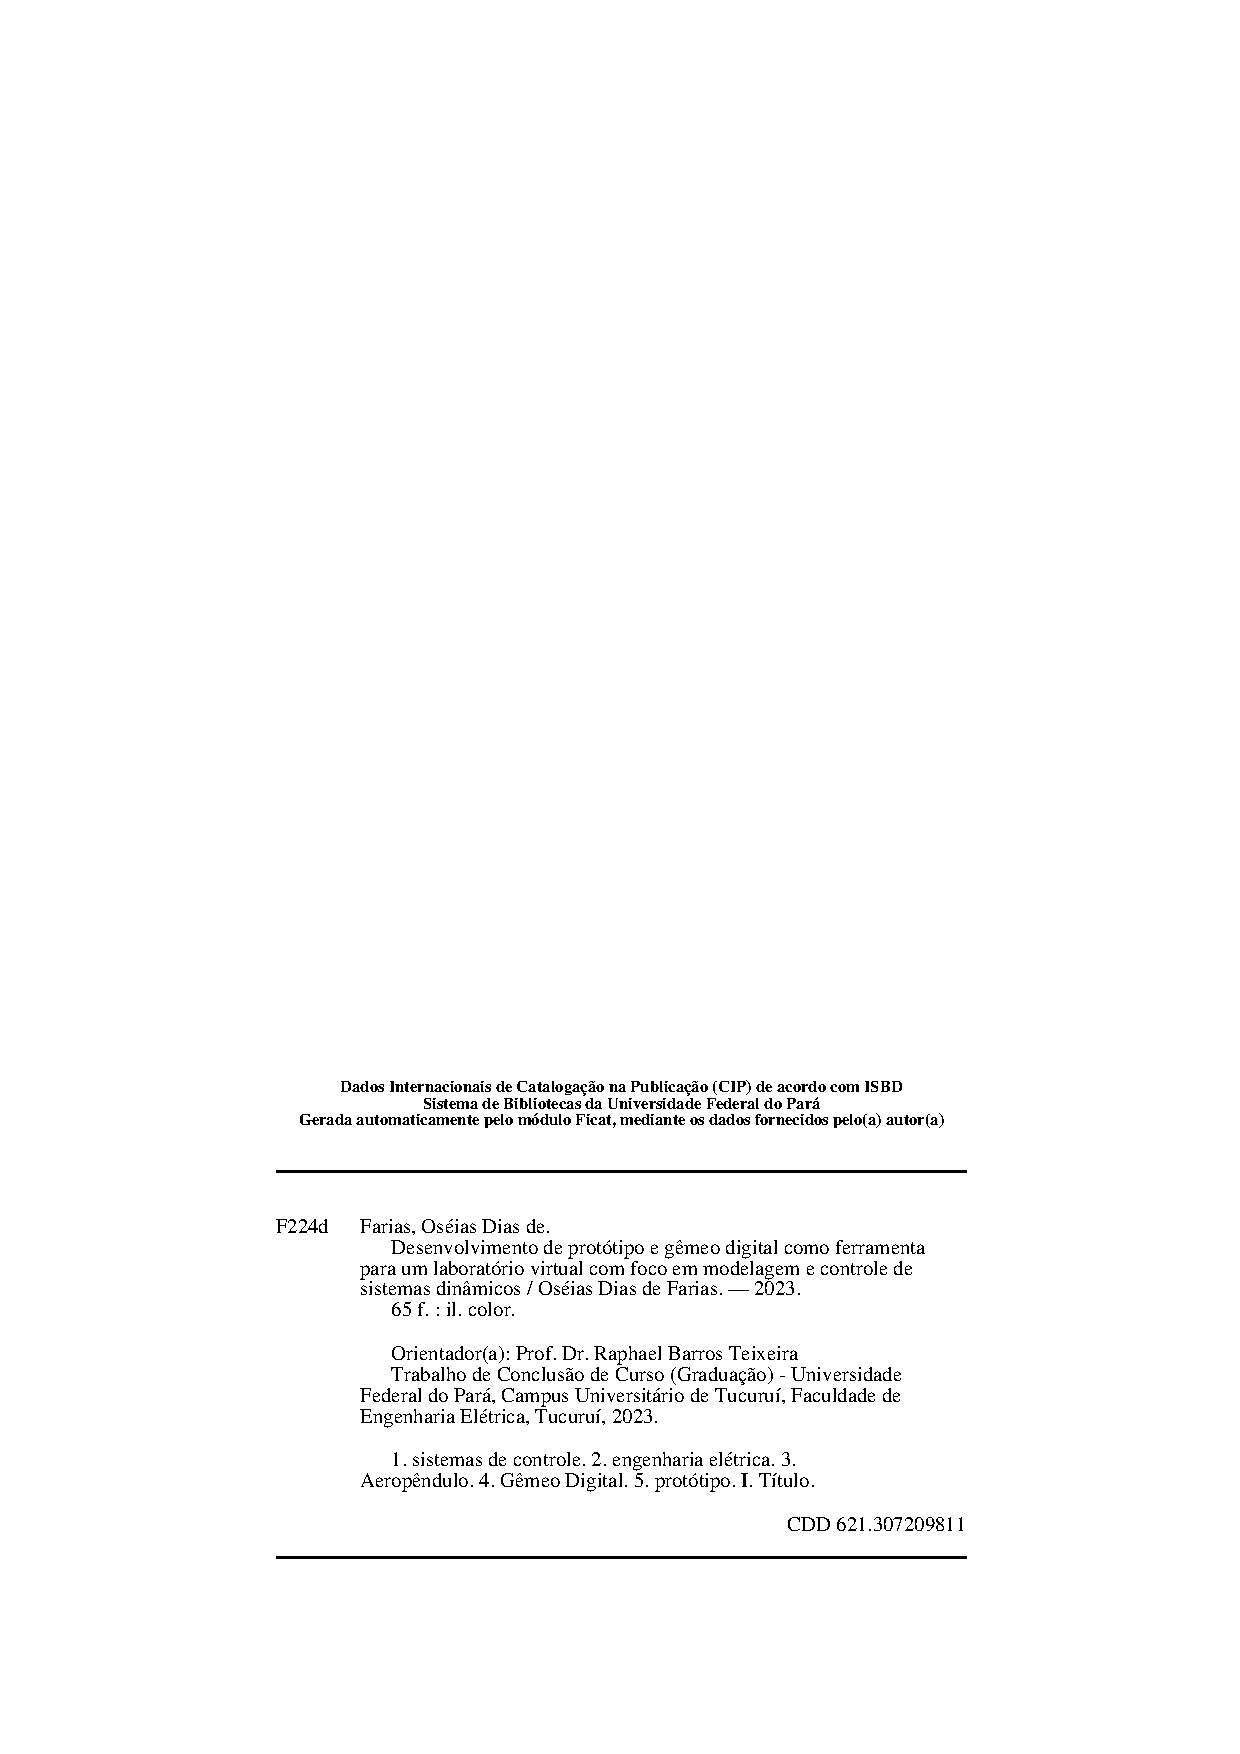
\includepdf[pages=-]{elementos_pretextuais/ficha_catalografica_UPFA.pdf}
%-------------------------------------Elementos pré-textuais:-------------------------------------
% Inserir folha de aprovação e ata de defesa
% -------------------------------------------------------------------------------------------------
% Informações de dados para a folha de aprovação
% -------------------------------------------------------------------------------------------------
\begin{folhadeaprovacao}
  \begin{center}
    {\ABNTEXchapterfont\imprimirautor}
      \vspace*{1cm}
    \begin{center}
      \ABNTEXchapterfont{\imprimirtitulo}
    \end{center}
       \vspace*{1cm} 
    \hspace{.45\textwidth}
    \begin{minipage}{.50\textwidth}
        \imprimirpreambulo
    \end{minipage}%
   \end{center}
\vspace*{1cm}       
\noindent Data de aprovação:  11 de Dezembro de 2023
\vspace*{1cm}
\begin{center}
\textbf{Banca Examinadora:}
\end{center}
% -------------------------------------------------------------------------------------------------
% -------------------------------------------------------------------------------------------------

%Editar apenas o nome dos participantes da banca examinadora:
   \assinatura{\textbf{\imprimirorientador} \\ Orientador - FEE/CAMTUC/UFPA} 
   \assinatura{\textbf{Prof. Dr. Rafael Suzuki Bayma} \\ Avaliador Interno - FEE/CAMTUC/UFPA}
   \assinatura{\textbf{Prof. Dr. André Felipe Souza da Cruz} \\ Avaliador Interno - FEE/CAMTUC/UFPA}
% -------------------------------------------------------------------------------------------------
% -------------------------------------------------------------------------------------------------
   
%   \vspace*{1cm}  
   \begin{center}
\vspace*{\fill}
	\vfill
    \imprimirlocal
    \par
    \imprimirdata
  \end{center}
\end{folhadeaprovacao}
% ---

\newpage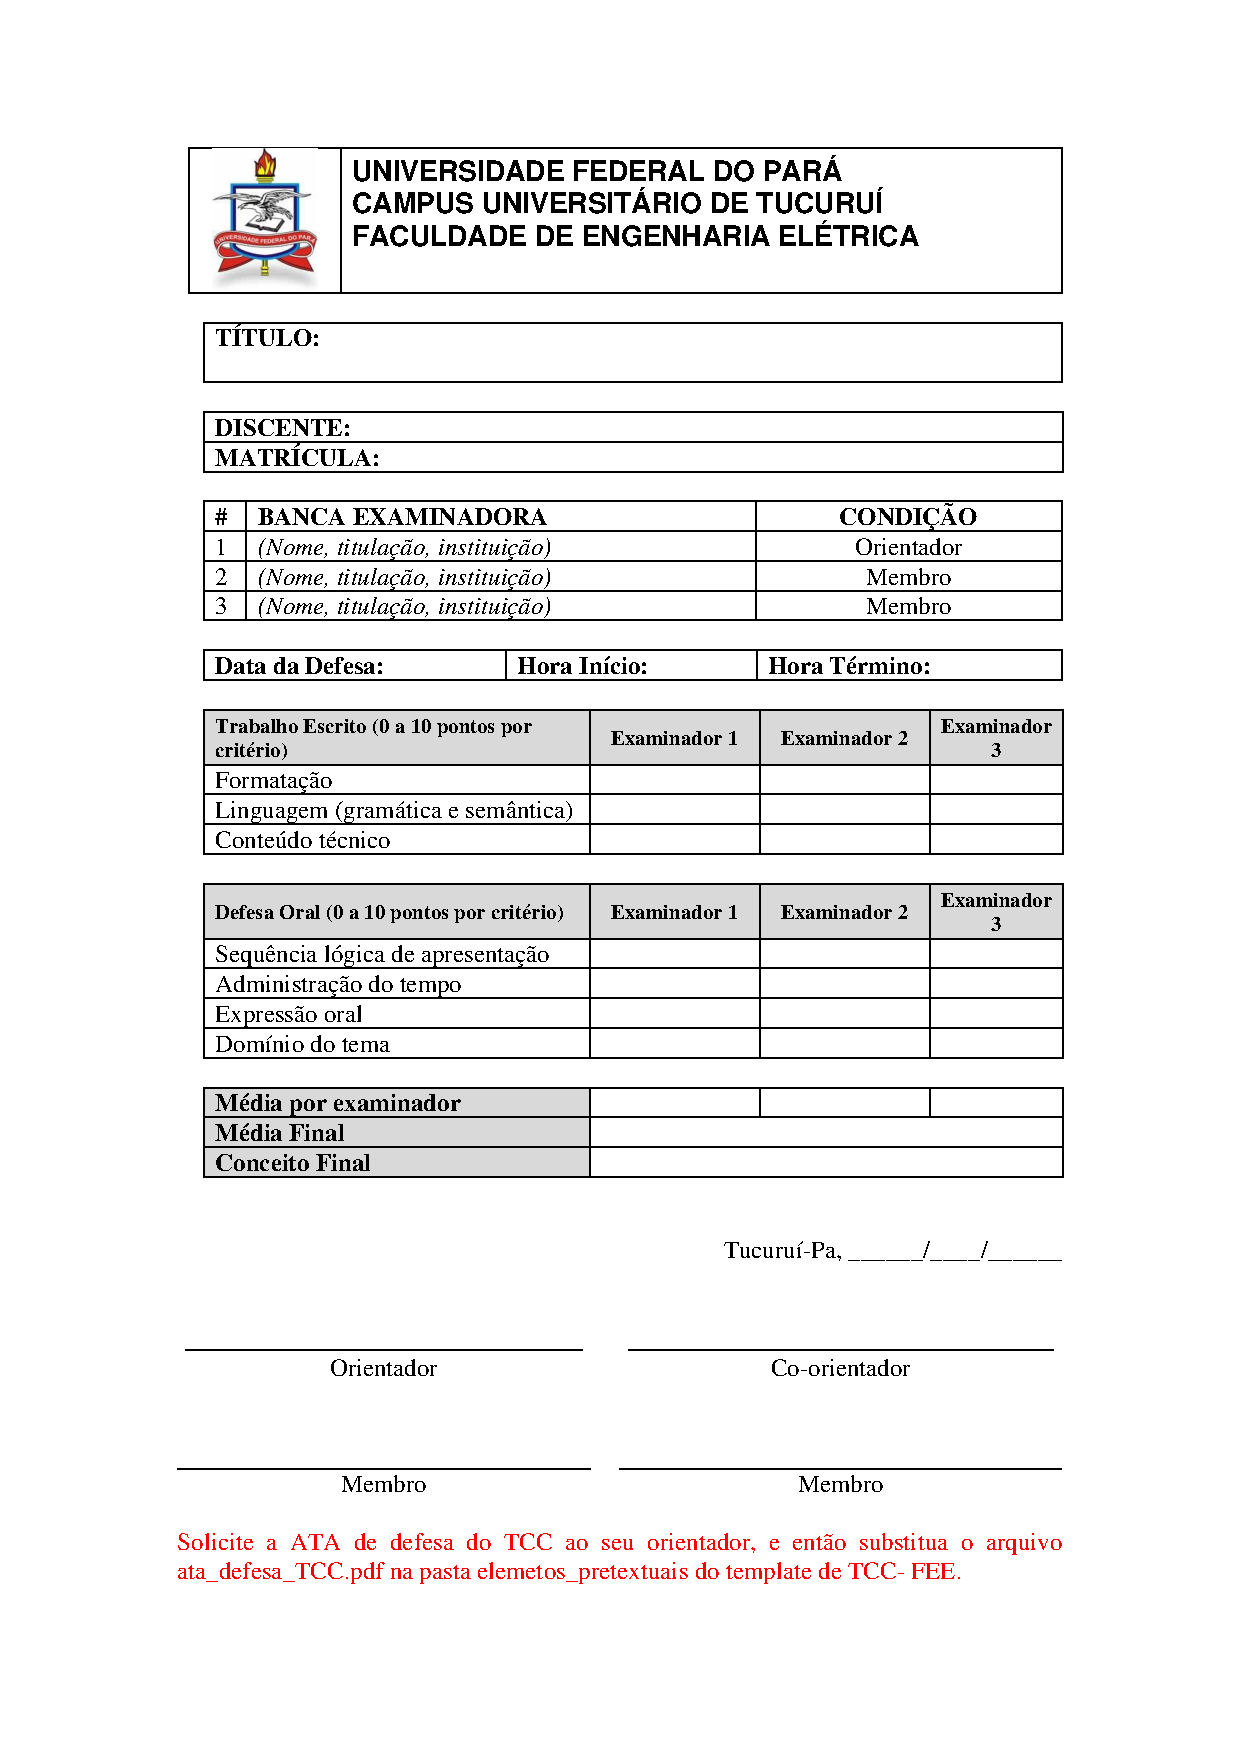
\includepdf[pages=-]{elementos_pretextuais/ata_defesa_TCC.pdf}
%---
% Inserir folha de dedicatória:
% -------------------------------------------------------------------------------------------------
% Inserir a dedicatória
% -------------------------------------------------------------------------------------------------

\begin{dedicatoria}
\begin{flushright}
\hspace{.45\textwidth}
\begin{minipage}{.55\textwidth}

Dedico a minha mãe, meu pai e a minhas irmãs,
além de todas as pessoas que me apoiaram nessa fase crucial da minha vida.

    \end{minipage}%
 \end{flushright}
\end{dedicatoria}


  
%---
% Inserir folha de agradecimentos:
% -------------------------------------------------------------------------------------------------
% Inserir os agradecimentos:
% -------------------------------------------------------------------------------------------------

\begin{agradecimentos}

À minha mãe e meu pai que dedicaram suas vidas por esse propósito, Aos professores do curso pela dedicação em simplificar o complexo, em especial aos professores da área de sistema de controle;\\
Finalmente, ao meu orientador Prof. Dr. Raphael Teixeira pela sua orientação e paciência.

\end{agradecimentos}
% ---

%---
% Inserir folha de epigrafe:
% EPÍGRAFE---------------------------------------------------------------------

\renewcommand{\epigraphname}{EPÍGRAFE}

\begin{epigrafe}

\textit{``A matemática é o alfabeto no qual Deus escreveu o universo.'' (Galileu Galilei)}

\end{epigrafe}

% OBSERVAÇÕES------------------------------------------------------------------
% Altere o texto para inserir a epígrafe do seu trabalho


%---
% Inserir Resumo e abstract:
% RESUMO---------------------------------------------------------

\begin{resumo}[\textbf{RESUMO}]
Este trabalho apresenta um laboratório virtual abrangente para o estudo de sistemas de controle, que combina a integração de um protótipo físico, simulador 3D e uma interface gráfica interativa. A motivação para este projeto reside na intrínseca complexidade associada à compreensão de sistemas de controle, que frequentemente apresenta desafios, sobretudo para estudantes que precisam transpor a barreira de abstrair sistemas físicos em termos de equações matemáticas. Para o desenvolvimento do projeto foi implementado um protótipo do Aeropêndulo completo com um conjunto de software que permite a interação do usuário com o sistema físico, possibilitando ao usuário realizar modificações nos parâmetros do sistema em tempo real, além disso, foi elaborado um gêmeo digital para espelhar a dinâmica do protótipo do Aeropêndulo a partir de um simulador 3D, por fim, foi realizado testes para a validação do laboratório, sendo eles: aplicação de identificação de sistema usando função de transferência discreta e mínimos quadrados e teste em malha fechada com controlador PID. O projeto foi hospedado no GitHub, a fim de disseminar o conhecimento e permitir que entusiastas, estudantes e pesquisadores tenham acesso ao projeto completo, A combinação de protótipos, simuladores, interface gráfica e integração de diversas disciplinas da Engenharia Elétrica cria um ambiente de aprendizado envolvente e eficaz para o estudo de sistemas de controle. Essa abordagem reduz a resistência inicial dos alunos e promove uma compreensão mais profunda dos conceitos e aplicações dessa área. Por meio da prática, os estudantes podem perceber a relevância das abstrações matemáticas na resolução de problemas reais, preparando-os para lidar com sistemas de controle complexos e desafiadores.\\

\textbf{Palavras-chave}: Aeropêndulo, identificação de sistema, protótipo, simulador, Gêmeo Digital.
\end{resumo}



% ABSTRACT--------------------------------------------
\begin{resumo}[\textbf{ABSTRACT}]

\textit{This work presents a comprehensive virtual laboratory for the study of control systems, which combines the integration of a physical prototype, 3D simulator and an interactive graphical interface. The motivation for this project lies in the intrinsic complexity associated with understanding control systems, which often presents challenges, especially for students who need to overcome the barrier of abstracting physical systems in terms of mathematical equations. To develop the project, an Aeropendulum prototype was implemented, complete with a set of software that allows the user to interact with the physical system, enabling the user to make changes to the system's parameters in real time. In addition, a digital twin was developed to mirror the dynamics of the Aeropendulum prototype using a 3D simulator. Finally, tests were carried out to validate the laboratory, including: application of system identification using discrete transfer function and least squares and closed loop testing with a PID controller. The project has been hosted on GitHub in order to disseminate knowledge and allow enthusiasts, students and researchers to have access to the complete project, The combination of prototypes, simulators, graphical interface and integration of various Electrical Engineering disciplines creates an engaging and effective learning environment for the study of control systems. This approach reduces students' initial resistance and promotes a deeper understanding of the concepts and applications in this area. Through practice, students can see the relevance of mathematical abstractions in solving real problems, preparing them to deal with complex and challenging control systems.}\\

\textbf{Keywords}: \textit{Aeropendulum, system identification, prototype, simulator, digital twin}.
\end{resumo}

%---
% Inserir lista de ilustrações (para remover a cor azul das partes com com hiperlink, modificar em "config_de_paginas.tex"):
\pdfbookmark[0]{\listfigurename}{lof}
\listoffigures*
\cleardoublepage 
%---
% Inserir lista de tabelas (para remover a cor azul das partes com com hiperlink, modificar em "config_de_paginas.tex"):
%\pdfbookmark[0]{\listtablename}{lot}
%\listoftables*
%\cleardoublepage
%---
%Inserir lista de quadros:
%\renewcommand{\listquadroname}{\textbf{LISTA DE QUADROS}}
%\renewcommand{\cftquadroname}{\quadroname\space} 
%\renewcommand*{\cftquadroaftersnum}{~~--}
%\counterwithout{quadro}{chapter}
%%---\pdfbookmark[0]{\listofquadrosname}{loq}
%\listofquadros*
%\cleardoublepage
%% --
% Inserir lista de abreviaturas e siglas, e simbolos:
%\begin{siglas}
    \item[{CPU}]{\textit{\textit{Central Processing Unit }}}
    \item[{PLD}]{\textit{\textit{Programmable Logic Device}}}
    \item[{SPLD}]{\textit{\textit{Simple Programmable Logic Device}}}
    \item[{CPLD}]{\textit{\textit{Complex Programmable Logic Device}}}
    \item[{ASIC}]{\textit{\textit{Application Specific Integrated Circuit}}}
    \item[{FPGA}]{\textit{\textit{Field Programmable Gate Arrays}}}
    \item[{VHDL}]{\textit{\textit{VHSIC Hardware Description Language}}}
    \item[{VHSIC}]{\textit{\textit{Very High Speed Integrated Circuit}}}
    \item[{HDL}]{\textit{\textit{Hardware Description Language}}}
\end{siglas}
%% ---



%\begin{simbolos}
	   
\item[$\boldsymbol{\mathcal{D}}$]             Densidade de Fluxo Elétrico Instantânea ($C/m^2$);

\item[$\boldsymbol{\mathcal{B}}$]              Densidade de Fluxo Magnético Instantânea ($Wb/m^2$);

\item[$\boldsymbol{\mathcal{E}}$]             Intensidade de Campo Elétrico Instantânea ($V/m$);

\item[$\boldsymbol{\mathcal{H}}$]              Intensidade de Campo Magnético Instantânea ($A/m$);
	   
\end{simbolos}





% -------------------------------------------------------------------------------------------------

% -----------------------------------------Inserir o sumario---------------------------------------
% Obs1: Para remover a cor azul das partes com com hiperlink, modificar em "config_de_paginas.tex"
% Obs2: Na versão final do trabalho, basta descomentar as linhas de 92 a 95 para incluir o sumário. Irá aparecer um erro devido a atualização de um dos pacotes, mesmo assim, após compilar duas vezes o código, o pdf será emitido noramalmente.
\pdfbookmark[0]{\contentsname}{toc}
\renewcommand\contentsname{\normalsize \textbf{SUMÁRIO}}
\tableofcontents*
\cleardoublepage
% -------------------------------------------------------------------------------------------------
% -------------------------------------------------------------------------------------------------

%-------------------------------------Elementos textuais:-------------------------------------
\textual
% ---
% Capítulo 01 - Introdução
%% INTRODUÇÃO------------------------------------------------------

\chapter{INTRODUÇÃO}\label{cap1}

Recentemente, tem-se notado um aumento significativo no número de aplicações que demandam cada vez mais processamento de dados, tais como mapeamento genético, computação gráfica, previsões meteorológicas e programas com grande quantidade de variáveis de entrada. \citeonline{dowd2010high} descrevem que a computação de alto desempenho é uma área que se preocupa em criar condições para executar processamentos com carga computacional elevada em intervalos de tempo viáveis.

Quando uma aplicação exige mais capacidade de processamento do que os computadores convencionais podem oferecer, é necessário buscar alternativas para criar sistemas de alto desempenho. Essa busca por soluções de processamento de alta performance é essencial para possibilitar a execução de programas complexos em um intervalo de tempo aceitável, e vem impulsionando o desenvolvimento de novas tecnologias de hardware e software. O uso de técnicas de processamento paralelo, computação distribuída e processamento em nuvem são exemplos de abordagens que visam a criação de sistemas computacionais de alto desempenho \cite{dowd2010high}. Essas tecnologias permitem que programas que levariam anos para fornecerem resultados em máquinas comuns possam ser executados em muito menos tempo, em questão de horas ou dias.

Uma abordagem diferente é a que consiste em construir circuitos orientados a aplicação, que são capazes de fornecer um bom desempenho para essa aplicação específica, ou seja, construir um hardware dedicado a essa aplicação. Por exemplo, é possível projetar e fabricar um circuito integrado específico (ASIC do inglês, \textit{Application Specific Integrated Circuit}) com o controle e as unidades funcionais personalizadas e otimizadas para uma dada aplicação. Com essa técnica de hardware dedicado pode-se atingir resultados muito bons com menos recursos de hardware \cite{Hager2017}. O ASIC é um circuito integrado para uma aplicação específica, tendo por objetivo solucionar demandas do mercado. Entretanto, cada projeto exige alto investimento, requerendo meses ou anos para ser desenvolvido, e fica limitado a uma dada aplicação. O desenvolvimento de ASICs é justificado comercialmente com um alto volume de produção, ou aplicações muito específicas, como em medicina (por exemplo, marcapasso) ou em aplicações militares.

Outra opção de dispositivo reconfigurável, é o FPGA (do inglês \textit{Field-programmable Gate Array}). Este é um dispositivo que permite a implementação de aplicações específicas. E contrastando com o ASICs, a implementação em FPGAs não é permanente, podendo ser reconfigurada de forma barata e fácil. Como vantagem, este apresenta baixa granularidade, permitindo a configuração em nível de porta lógica. Isso significa que é possível criar virtualmente qualquer circuito digital a partir de uma descrição em HDL (do inglês, \textit{Hardware Description Language}). 

Assim como um computador, o FPGA é capaz de executar milhões de operações simultâneas, tornando-o potencialmente centenas de vezes mais rápido do que projetos baseados em microprocessadores, devido à possibilidade de explorar o paralelismo espacial oferecido pelos elementos configuráveis presentes nos dispositivos atuais. 

FPGAs podem ser utilizados em diversas aplicações de sistemas embarcados, como no setor automotivo, médico, industrial, equipamentos de imagem e telecomunicações, por exemplo. Compete ao meio acadêmico e a indústria realizar estudos e incentivos para utilizar a combinação: lógica programável com processadores embarcados. Dado o crescente destaque deste campo de atuação, é interessante que conceitos de programação reconfigurável sejam introduzidos ao ensino de automação e eletrônica. Desta forma, este trabalho busca contribuir com o ensino de Engenharia, utilizando o kit FPGA DE2-115 da Altera, por meio de uma abordagem pratica obtida pela criação e execução de roteiros aplicáveis em sala de aula. O DE2-115 é uma placa de desenvolvimento que incorpora uma FPGA da Altera, juntamente com uma variedade de periféricos e interfaces, tornando-o ideal para projetos de automação. Isso permite que os estudantes aprendam conceitos importantes, como programação em VHDL (VHSIC\textit{ Hardware Description Language}), design de sistemas digitais, interfaceamento com sensores e atuadores, e implementação de lógica de controle em hardware. Os estudantes podem projetar e implementar sistemas de automação em tempo real, utilizando a plataforma FPGA para desenvolver circuitos personalizados e reconfiguráveis.

Através do ensino de automação utilizando o DE2-115, os estudantes podem adquirir habilidades práticas e relevantes para a indústria, como design de sistemas embarcados, programação de dispositivos reconfiguráveis, desenvolvimento de algoritmos de controle em hardware e integração de sistemas de automação com o mundo físico. Além disso, o uso do DE2-115 pode incentivar a criatividade e a inovação, permitindo que os estudantes projetem soluções personalizadas para problemas específicos de automação.


\section {Justificativa}

O uso de hardware reconfigurável permite a operação dedicada a um objetivo específico, sem influência de outros processos em concorrência, o que resulta em ganho de desempenho e processamento dedicado para a execução de algoritmos. É essencial que os profissionais de engenharia elétrica sejam introduzidos a ferramentas de programação digital, especialmente para análise e aplicação em campos como telecomunicações. No entanto, muitos estudantes enfrentam dificuldades nesses temas de estudo devido à escassez de materiais de ensino disponíveis. Portanto, esse trabalho propõe o desenvolvimento de material de ensino da linguagem VHDL, visando sua implementação em componentes curriculares de eletrônica digital e telecomunicações. 
 

\section{Objetivos}

Este trabalho tem como objetivo, propor a criação de material didático, e de fácil compreensão, para ensino de automação a partir de Dispositivos Lógicos Programáveis, utilizando um Kit de Aprendizado e Desenvolvimento FPGA (DE2-115), programado via VHDL.

Para alcançar o objetivo proposto, foram definidas seguintes metas:

\begin{enumerate}[label={\noNalph{enumi})}]
    \item Realizar uma revisão bibliográfica sobre os fundamentos de sistemas digitais e lógica de programação;
    \item Estudar a implementação de códigos em VHDL;
    \item Estudar o funcionamento do FPGA DE2-115 da Altera;
    \item Propor roteiros experimentais para estudo de lógica combinacional e sequencial;
    \item Documentar os resultados obtidos, contribuindo com o ensino de sistemas digitais e eletrônica reconfigurável.”
\end{enumerate}

\section{Estrutura da Monografia}
Este trabalho está estruturado em seis capítulos.

O capítulo \ref{cap1} é introdutório, neste são apresentados a justificativa, objetivos e estrutura do trabalho desenvolvido.

No capítulo 2 é apresentada a fundamentação teórica sobre sistemas digitais, lógica programável e dispositivos lógicos programáveis.

O capítulo 3 reúne as principais partes e funcionamento do kit FPGA DE2-115 da Altera.

No capítulo 4 são apresentados os roteiros experimentais que poderão ser aplicados para ensino de automação utilizando sistemas lógicos programáveis.

O capítulo 5 apresenta os resultados obtidos a partir da execução dos experimentos descritos no capítulo 4.

Finalmente, no capítulo 6 são apresentadas as considerações finais e perspectivas de trabalhos futuros

%==============================================================%



\chapter{Introdução}
\label{ch:intro}

\section{Justificativa}

Os sistemas de controle desempenham um papel fundamental na sociedade contemporânea, permeando uma ampla gama de aplicações ao nosso redor. Desde o lançamento de foguetes e o decolamento do ônibus espacial até processos de usinagem automatizados, onde peças metálicas são trabalhadas envoltas em jatos de água de resfriamento, até veículos autônomos que distribuem materiais em oficinas aeroespaciais, a presença e a influência dos sistemas de controle automático são evidentes, \cite{nise2013}. É crucial ressaltar que, ao realizar análises e projetar controladores eficazes para tais sistemas, é necessário realizar uma abstração desses sistemas físicos por meio de equações matemáticas. Essa prática, embora essencial, pode tornar a interpretação desafiadora para iniciantes na área devido à complexidade intrínseca das formulações matemáticas envolvidas.

Além disso, a implementação de controladores requer competência em diferentes áreas da engenharia, tais como eletrônica analógica e digital, programação, processamento de sinais, circuitos elétricos, entre outras. Dessa forma, torna-se necessário integrar conhecimentos multidisciplinares para a implementação bem-sucedida de controladores em sistemas reais.

Um sistema de controle é composto por subsistemas e processos, concebidos com a finalidade de alcançar uma saída desejada com um desempenho específico, considerando uma entrada predefinida, \cite{nise2013}.

A abordagem convencional no ensino das disciplinas teóricas em cursos de Engenharia representa um desafio significativo, dada a dificuldade dos alunos em estabelecer conexões entre o conteúdo teórico e a aplicação prática nos sistemas físicos. A introdução de tecnologias de apoio tem proporcionado avanços, mas persistem desafios, como a carência de estrutura operacional e a necessidade de atualização nas metodologias de ensino. A incorporação de simulações computacionais aliadas a animações emerge como uma estratégia promissora para acelerar esse processo, oferecendo uma ponte eficaz entre a teoria e a compreensão prática, \cite{yuri_tcc}.

No entanto, no estudo de sistemas de controle, é comum que os discentes enfrentem desafios em seu primeiro contato com a área, especialmente devido à necessidade de aplicar abstrações matemáticas para representar a dinâmica de sistemas físicos. Essa etapa inicial pode parecer complexa, porém é crucial para a compreensão e domínio dos conceitos fundamentais envolvidos na análise e controle de sistemas.

Uma das principais razões pelas quais os estudantes encontram dificuldades é a transição do mundo físico para o mundo matemático abstrato, onde os sistemas são modelados por equações diferenciais, transformadas de Laplace e outros formalismos matemáticos. Para muitos, essa mudança pode parecer distante da realidade observada, o que pode causar alguma resistência inicial.

Assim, buscando superar essa barreira de aprendizagem, é fundamental desenvolver métodos que possibilitem aos discentes visualizar a dinâmica desses sistemas na prática. Uma abordagem promissora é a utilização de protótipos, que permitem aos alunos observar a dinâmica analisada matematicamente no mundo real. Essa aplicação prática fornece uma conexão mais tangível entre os conceitos abstratos e suas aplicações concretas, tornando o aprendizado mais envolvente e compreensível.

Adicionalmente, o uso de simuladores pode ser altamente benéfico. Ao inserir as respostas obtidas por meio dos modelos matemáticos como entrada nos simuladores, o processo de aprendizado integra ferramentas matemáticas e de visualização. Dessa forma, os alunos podem interagir com os sistemas em diferentes cenários, observando como as variáveis influenciam o comportamento dos sistemas de controle. Essa abordagem interativa e experimental ajuda a solidificar conceitos e aprimorar a compreensão do funcionamento desses sistemas complexos.

Ao combinar a teoria matemática com a prática através de protótipos e simuladores, o processo de aprendizado torna-se mais fluido e estimulante. Os alunos podem perceber a relevância das abstrações matemáticas na resolução de problemas reais, o que reduzirá a resistência inicial e aumentará o interesse pela área de sistemas de controle.

A proposta deste trabalho consiste no desenvolvimento de um protótipo que utiliza um conjunto de softwares para criar um laboratório virtual. Essa abordagem possibilita que os estudantes construam seu próprio laboratório de maneira ágil e flexível, utilizando componentes acessíveis e softwares de código aberto, sem custos adicionais. Dessa forma, os estudantes têm a oportunidade de aprimorar seus conhecimentos e aprofundar tanto a teoria quanto a prática de forma complementar, resultando em uma base de aprendizado mais sólida.

O projeto compreende um protótipo de Aeropêndulo composto por firmware para o microcontrolador, software de usuário e um simulador 3D. Este protótipo foi concebido com a premissa de ter o menor custo possível, visando proporcionar aos interessados uma implementação acessível com gastos mínimos em componentes. O algoritmo do firmware foi desenvolvido em linguagens C e C++, utilizando o Framework do Arduino em conjunto com o PlatformIO e o microcontrolador ESP32.

A interface do usuário foi projetada com o objetivo de simplificar a interação em tempo real, permitindo ajustes nos parâmetros do sinal de referência durante a execução do sistema. Por fim, foi criado um gêmeo digital do protótipo físico, possibilitando a observação da dinâmica do sistema físico por meio de um simulador 3D. Este simulador replica o comportamento do protótipo em tempo real, proporcionando uma integração eficaz entre o mundo real e o computacional.

Conforme destacado por Grieves (2014) em sua pesquisa pioneira na Universidade de Michigan, o conceito de 'gêmeo digital' permeia todas as fases do ciclo de vida de um produto, desde o protótipo até a operação, proporcionando uma abordagem abrangente para avaliar a performance e desgaste no mundo real. Este estudo concentra-se na aplicação deste conceito na etapa de operação e manutenção, enquanto ressalta a relevância de explorar seu potencial em outras fases do ciclo de vida do produto\cite{quinalha2018gemeos}.


\section{Objetivos}

\subsection{Objetivos Gerais}

Este trabalho tem como objetivo desenvolver um laboratório virtual abrangente para o estudo de sistemas de controle. Para alcançar esse propósito, será criado um projeto que integra um protótipo, simulador e uma interface gráfica, possibilitando sua utilização na investigação de diversos aspectos e subáreas relacionadas a sistemas de controle. Isso inclui a identificação de sistemas, o desenvolvimento de controladores, a otimização de controladores, bem como a aplicação de Inteligência Artificial em sistemas de controle, entre outros tópicos.

Além disso, a proposta envolve a aplicação prática dos conhecimentos adquiridos durante a graduação, unindo técnicas de sistemas de controle, eletrônica analógica e digital, programação, física e cálculo em uma configuração de sistema físico. O principal objetivo é criar um ambiente que permita ao pesquisador aplicar e aprimora seus conhecimentos e observar o comportamento da dinâmica do sistema em um ambiente real. Para realizar essa tarefa, será necessário combinar tecnologias de diversas disciplinas do curso de Engenharia Elétrica, tornando o projeto ainda mais intrigante e desafiador.


\subsection{Objetivos Específicos}

\begin{itemize}
        \setlength{\itemsep}{-2pt}
	\item \textbf{Desenvolver o protótipo do Aeropêndulo}: Projetar a estrutura física e elétrica do sistema;
        \item \textbf{Desenvolver um simulador 3D (Gêmeo Digital)}: programar o simulador usando a linguagem de programação Python em conjunto com a biblioteca VPython;
        \item \textbf{Interface de Usuário}: Desenvolver uma interface gráfica com menu para manipular o comportamento do sistema em tempo real, salvar dados de ensaio e testar o sistema em malha fechada;
        \item \textbf{Aplicar Identificação de sistema a Planta}: Obter um modelo da planta usando função de transferência discreta  por identificação de sistemas usando o método dos mínimos quadrados;
        \item \textbf{Testar o sistema  em Malha Fechada}: Implementar um controlador PID junto do firmware e realizar testes para validar o sistema em malha fechada;
\end{itemize}


\section{Escopo do Trabalho}

O projeto parte de uma modelagem matemática usando como base os princípios da física newtoniana com o intuito de demostrar que para sistemas relativamente complexos, essa técnica de modelagem pode se tornar trabalhosa e por muitas vezes impraticáveis, a partir dessa premissa parte-se para o desenvolvimento do protótipo, o objetivo está na utilização do sistema físico para aplicar o método de identificação de sistema que consiste em obter um modelo matemático, que descreva a dinâmica do sistema físico de forma aproximada, a partir dos dados de entrada e saída do protótipo.

No processo de condução dos ensaios e na aquisição dos dados essenciais para a realização dos estudos, o projeto inclui o desenvolvimento de uma interface gráfica. Esta interface capacita o pesquisador a executar ensaios e a armazenar os dados obtidos, viabilizando a subsequente modelagem e análise do comportamento do sistema em estudo. Adicionalmente, a interface é equipada com um menu que permite a configuração em tempo real dos ensaios para diferentes sinais de entrada, além da configuração dos parâmetros de frequência, amplitude e offset. Essa funcionalidade dinâmica e flexível aprimora significativamente a condução da pesquisa, tornando-a mais produtiva e eficiente.

Além da interface gráfica executada no computador, é fundamental o desenvolvimento de um firmware que gerencie aspectos cruciais, como a comunicação, aquisição de dados e controle do Aeropêndulo. Essas funcionalidades são implementadas por um microcontrolador. Este microcontrolador não apenas estabelece a comunicação com a interface gráfica através da conexão USB, mas também desempenha um papel vital na geração dos sinais de entrada para a planta e na leitura do ângulo do braço do Aeropêndulo.


Além disso, o projeto incorpora um gêmeo digital do sistema físico, na forma de um simulador 3D do Aeropêndulo. Essa abordagem permite a integração da dinâmica do sistema real com o ambiente computacional, possibilitando a recriação em tempo real da planta de forma virtual. Essa simulação em 3D não apenas enriquece a experiência de aprendizado, mas também oferece aos estudantes a oportunidade de se envolver em um processo de aprendizado prático que se assemelha significativamente às condições do mundo real. Isso resulta em um processo educacional mais imersivo e eficaz, capacitando os alunos a compreender e explorar a complexidade dos sistemas de controle de maneira mais aprofundada.

A seção \ref{fundamentacao_teorica} desenvolve a fundamentação teórica focando na modelagem matemática do sistema, a seção \ref{implementacao_prototipo} implementa o protótipo de Aeropêndulo mostrando passo a passo o processo de desenvolvimento até a concepção da planta, para o desenvolvimento dos softwares a seção \ref{dev_softwares} descreve as etapas do desenvolvimento das aplicações, finalizando o capítulo \ref{cap_desenvolvimento} a seção \ref{flu_lab_virtual} descreve as partes do laboratório a partir de um fluxograma do sistema.

O capítulo \ref{cap_3} aborda os resultados e discussões obtidos ao término do projeto. Na seção \ref{indentificacao}, emprega-se o método de identificação de sistemas para validar a estrutura de obtenção e armazenamento dos dados de ensaio. Adicionalmente, a seção \ref{malha_fechada} implementa um controlador PID simples com o propósito de validar a infraestrutura física e de software desenvolvida para os testes de controladores na planta física.

Por fim, o capítulo \ref{cap_conclusao} consolida os avanços alcançados no projeto, destacando perspectivas futuras para sua aplicação. Na seção \ref{concideracoes_finais}, são apresentadas considerações finais sobre a implementação realizada. Além disso, a seção \ref{trabalhos_futuros} oferece uma visão prospectiva sobre possíveis trabalhos futuros que podem adotar o projeto desenvolvido neste trabalho como ambiente de estudo.



% ---
% Capítulo 02 - Resumo Teórico
%% REVISÃO DE LITERATURA-------------------------------------------
\chapter{DISPOSITIVOS LÓGICOS E LÓGICA PROGRAMÁVEL}
\label{cap2}

A lógica programável é um campo que se baseia em princípios e conceitos que permitem a criação de soluções de hardware por meio do uso de dispositivos programáveis. Esses dispositivos são capazes de executar funções lógicas específicas, as quais podem ser definidas pelo fabricante ou pelo usuário, utilizando tanto software quanto hardware.
Além disso, a lógica programável tem sido amplamente utilizada em diversos campos, como em sistemas embarcados \cite{mishra2018fpga}, comunicações digitais \cite{proakis2006digital}, processamento de sinais \cite{shynk1999review}, entre outros. Esses avanços têm sido possíveis graças aos esforços contínuos de pesquisa e desenvolvimento em hardware e software. De acordo com \citeonline{brown2013field}, os dispositivos programáveis podem ser classificados em várias categorias, dependendo do nível de abstração e da tecnologia utilizada. 

\section{Introdução aos Dispositivos Lógicos Programáveis}

Na década de 1970, surgiram no mercado os dispositivos lógicos programáveis (PLD), que revolucionaram a área de circuitos lógicos combinacionais. Um PLD é basicamente um tipo de chip para uso geral que possui hardware configurável e/ou reconfigurável, em contraste com os microprocessadores, que executam programas por meio de hardware fixo \cite{pedroni2010eletronica}. Dentro da categoria de PLDs, há uma ampla variedade de chips disponíveis, sendo a maioria deles agrupados sob o termo Dispositivos Lógicos Programáveis Simples (SPLD). No entanto, os mais relevantes e conhecidos são os Dispositivos Lógicos Programáveis Complexos (CPLD), os Arranjos de Portas Programáveis em Campo (FPGA) e os Circuitos Integrados de Aplicação Específica (ASIC) \cite{moore2017fpgas}. 

\subsection{SPLD e CPLD}
Geralmente, um SPLD é utilizado em aplicações que exigem menos complexidade, como projetos de pequeno porte. Existem vários tipos de SPLDs disponíveis no mercado, incluindo PALs (\textit{Programmable Array Logic}) e GALs (\textit{Generic Array Logic}). Cada um desses tipos tem suas próprias características e vantagens, tornando-os adequados para diferentes aplicações \cite{floyd2009sistemas}. Já o CPLD é um dispositivo eletrônico programável que permite a criação de circuitos lógicos complexos em um único componente. Eles são compostos por vários SPLDs interconectados por meio de um arranjo complexo e programável. A Figura \ref{fig:Arqui_CPLD} ilustra a estrutura de um CPLD convencional \cite{pedroni2010eletronica}. Essa estrutura possibilita uma maior capacidade para projetar circuitos lógicos maiores e mais complexos do que os que poderiam ser criados com apenas um SPLD.

\begin{figure}[!htb]
    \centering
    \caption{Arquitetura básica de CPLDs}
    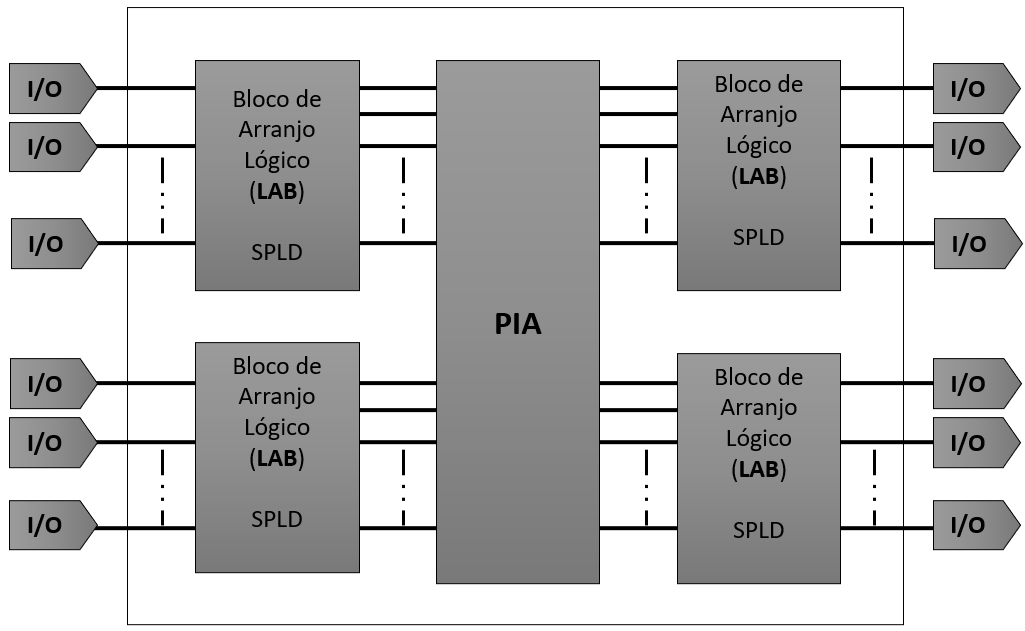
\includegraphics[scale=0.5]{figuras/ARQ_CPLD2.png}\\
    {\footnotesize Fonte: Adaptado de \cite{floyd2009sistemas}.}
    \label{fig:Arqui_CPLD}
\end{figure}

O CPLD pode ser reprogramado a qualquer momento, permitindo que o circuito seja atualizado e adaptado às necessidades do projeto. Cada arranjo SPLD em um CPLD é chamado de Bloco de Arranjo Lógico (LAB), que é uma unidade lógica programável que pode executar funções lógicas complexas. Cada LAB é interconectado por linhas de interconexão programáveis, chamadas de Arranjo de Interconexões Programáveis (PIA). Essas interconexões programáveis permitem que os blocos lógicos se comuniquem entre si e formem circuitos digitais complexos e customizados \cite{floyd2009sistemas}. 

Com esta classe de PLD, é possível implementar funções digitais de média e alta complexidade, incluindo sistemas sequenciais e combinacionais, como registradores de deslocamento, contadores, multiplexadores e decodificadores. Além disso, eles são frequentemente utilizados em aplicações de alta velocidade, como em sistemas de processamento de sinais digitais, processamento de imagens e em sistemas de controle de automação industrial \cite{pedroni2010eletronica} .

\subsection{FPGA}
Um FPGA, em tradução, um Arranjo de Portas Programáveis em Campo, é um dispositivo lógico que possui uma estrutura interna ainda mais complexa que um CPLD. \citeonline{ordonez2003projeto} afirma que a estrutura fundamental de um FPGA pode variar entre fabricantes, famílias de dispositivos e até mesmo dentro de uma mesma família, mas existem alguns elementos essenciais que são mantidos, como é mostrado na Figura \ref{fig:fpga_01}, os três elementos básicos que constituem um FPGA são :

\begin{enumerate}[label={\noNalph{enumi})}]
    \item CLB (\textit{Configurable Logic Block}): Blocos Lógicos Configuráveis, unidade lógica de um FPGA; 
    \item SB (\textit{Switch Box}): Caixa de Conexão, responsável pela conexão entre os CLBs,  através de canais de roteamento;
    \item IOB (\textit{In/Out Block}): Blocos de Entrada/Saída, responsáveis pela interface com o ambiente.
\end{enumerate}


\begin{figure}[!htb]
    \centering
    \caption{Representação dos elementos básicos de um FPGA}
    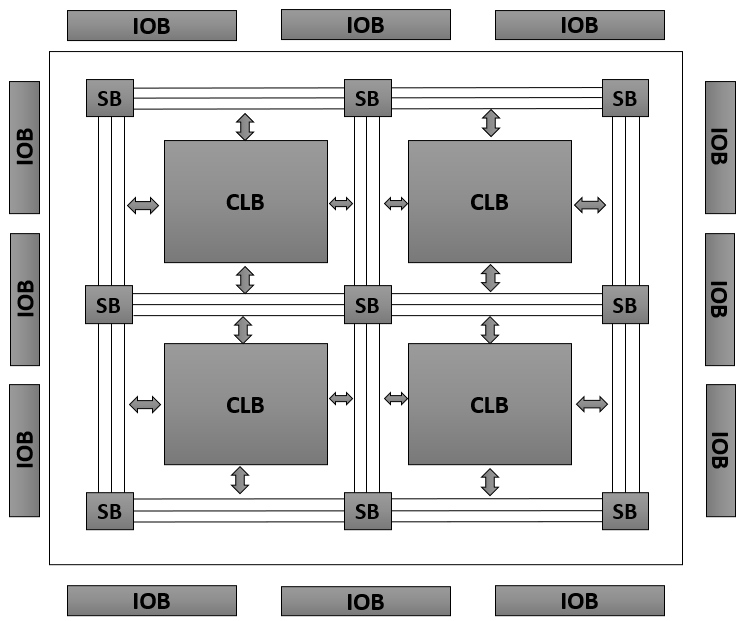
\includegraphics[height = 9cm]{figuras/fpga_2.png}\\
    {\footnotesize Fonte: Adaptado de \cite{floyd2009sistemas}}
    \label{fig:fpga_01}
\end{figure}

A característica programável em um FPGA é semelhante à interconexão de chaves em uma placa de prototipagem que pode ser alterada pelo projetista. No FPGA, essa interconexão pode ser reprogramada pelo usuário ou pelo designer no laboratório ou em campo. Isso é possível porque o FPGA é composto por uma matriz de células lógicas, que podem ser programadas para executar funções específicas, como portas lógicas, registradores, memórias, entre outras. A programação é feita através de um processo de configuração que pode ser realizado sem a necessidade de retirar o dispositivo do circuito, o que significa que é possível atualizar ou reconfigurar o FPGA sem ter que substituir o hardware \cite{roth2004circuit}. Por isso, essa matriz de portas lógicas (\textit{Gate Array}) é chamada de programável em campo (\textit{Field Programmable}). Os tipos de portas lógicas programáveis incluem todas as portas básicas para atender a qualquer necessidade \cite{SmithFranzon08}. 

\subsubsection{Blocos Lógicos Configuráveis (CLB)}

Os blocos lógicos configuráveis são uma das principais unidades funcionais dos FPGA. Cada CLB consiste em uma rede de células lógicas com a lógica desejada, além de possuir uma variedade de elementos de armazenamento, tais como flip-flops, latches e registradores. A arquitetura interna dos CLBs varia entre os fabricantes de FPGA, mas em geral eles possuem recursos de roteamento programáveis que permitem a interconexão entre os CLBs e outros blocos funcionais do FPGA. A figura \ref{fig:clb_bloc} ilustra a disposição dos CLBs essenciais nas interconexões programáveis globais em linha/coluna. Essas interconexões têm a função de estabelecer as conexões necessárias para interligar os blocos lógicos entre si. \cite{roth2004circuit}.

Os CLBs possuem grande flexibilidade, permitindo que os designers de hardware personalizem a lógica interna de acordo com as necessidades de seus projetos. Isso é possível através da programação do FPGA por meio de linguagens de descrição de hardware (HDL), como o VHDL, que permite a descrição da lógica desejada em um nível de abstração alto e
portável entre diferentes fabricantes de FPGA \cite{silva2013introducao}.

\begin{figure}[!ht]
    \centering
    \caption{Blocos lógicos configuráveis básicos (CLBs) dentro de interconexões programáveis globais em linha/coluna.}
    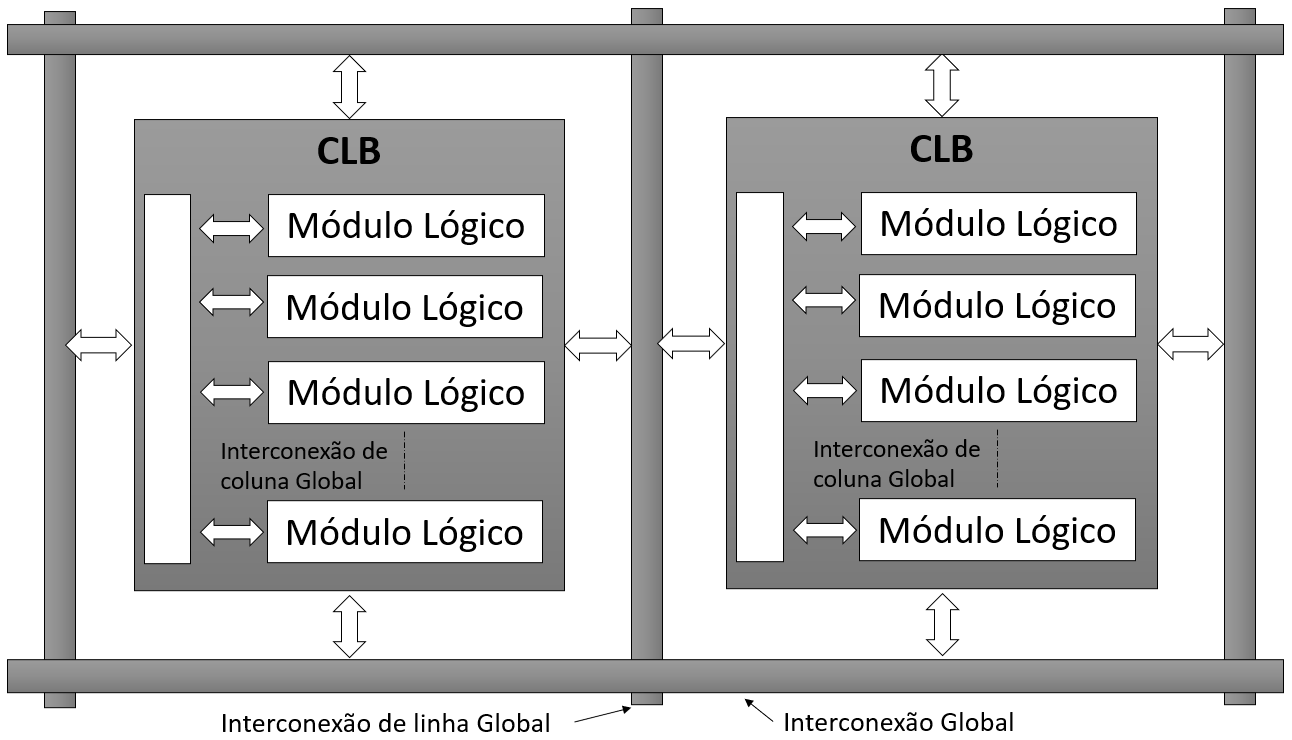
\includegraphics[height = 7.5cm]{figuras/clb_bloc0.png}\\
    {\footnotesize Fonte: Adaptado de \cite{floyd2009sistemas}}
    \label{fig:clb_bloc}
\end{figure}

Cada CLB em um FPGA é composto por vários módulos lógicos menores e uma interconexão programável local que permite a conexão entre esses módulos dentro do CLB. Esses módulos lógicos podem ser configurados como lógica combinacional, lógica registrada ou uma combinação de ambas. A Figura \ref{fig:mod_log} ilustra o diagrama em bloco de um módulo lógico típico baseado em LUT (\textit{Look Up Table}). Uma LUT, ou tabela de busca, é uma forma de memória programável utilizada para gerar funções lógicas combinacionais em formato de soma-de-produtos \cite{floyd2009sistemas}.

\begin{figure}[!ht]
    \centering
    \caption{Modulo Lógico.}
   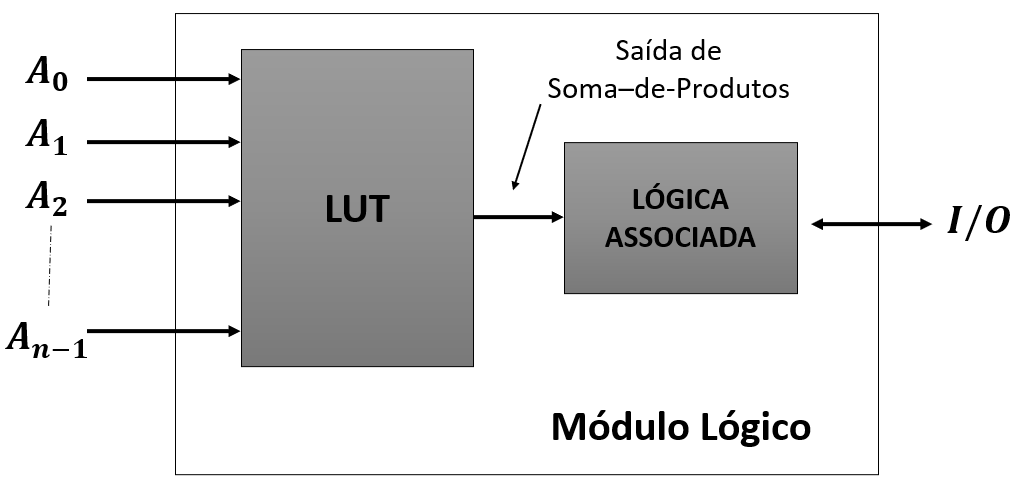
\includegraphics[height = 5.5cm]{figuras/Mod_log.png}\\
    {\footnotesize Fonte: Adaptado de \cite{floyd2009sistemas}}
    \label{fig:mod_log}
\end{figure}

\subsubsection{Caixa de Conexões (SB)}

As Caixas de Conexões servem para unir as interconexões programáveis, sendo estas responsáveis por estabelecer a conexão entre os CLBs e os blocos de entrada/saída (IOB) para implementar a lógica digital desejada. Essas interconexões são constituídas por um conjunto de elementos programáveis, como chaves, multiplexadores e buffers, que permitem a configuração do caminho de sinal entre os blocos
\cite{brown1992field}.

Além disso, a disposição das interconexões também é importante para o desempenho e eficiência do FPGA. Por exemplo, a utilização de canais de roteamento que permitem a
comunicação vertical e horizontal entre os CLBs, além de reduzir a latência e minimizar a interferência entre os sinais, também possibilita a implementação de circuitos mais complexos \cite{wong2007introduction}.

\subsubsection{Blocos de Entrada e Saída (IOB)}

Os blocos de entrada e saída são responsáveis por fornecer uma interface entre o circuito digital do FPGA e o mundo externo. Eles permitem com que haja a comunicação entre dispositivos, como sensores, atuadores, processadores e outros circuitos digitais.Estes são projetados para serem configuráveis e suportar vários padrões de comunicação, como interfaces seriais, paralelas e diferencias, entre outras. Eles são compostos por circuitos específicos, como registradores, buffers, multiplexadores e transceptores, que são configuráveis para atender às necessidades do projeto \cite{brown2013field, maxfield2004design}.

A organização dos blocos de entrada e saída varia de acordo com a arquitetura do dispositivo e a família do FPGA. Por exemplo, alguns FPGA possuem blocos de entrada e saída dedicados que são alocados em áreas específicas do dispositivo, enquanto outros possuem blocos de entrada e saída espalhados por toda a matriz de lógica do dispositivo \cite{xilinx2021ultrascale}.

\section{Linguagem de Descrição de Hardware - HDL}

Dispositivos lógicos programáveis, como os FPGAs, requerem o uso de uma linguagem específica para implementar circuitos físicos em seu próprio hardware. Essa linguagem é conhecida como Linguagem de Descrição de Hardware (HDL) \cite{ordonez2003projeto}.

As HDLs são estruturadas de forma a permitir a descrição abstrata do comportamento de hardwares, possibilitando a modelagem e representação da estrutura e funcionamento de circuitos em diferentes níveis de abstração durante o processo de projeto \cite{ordonez2003projeto}. Isso oferece aos projetistas maior flexibilidade na descrição de circuitos complexos. Anteriormente, essas linguagens eram comumente empregadas para a verificação de lógica. No entanto, com o surgimento dos algoritmos de síntese lógica, tornou-se viável descrever o fluxo de dados dos circuitos em níveis de transferência de registradores (RTL), simplificando a descrição de circuitos digitais. Com isso, detalhes como portas lógicas e interconexões passaram a ser processados automaticamente pelos algoritmos de síntese lógica. \cite{costa2014desenvolvimento}. 

As linguagens de descrição de hardware oferecem várias vantagens em relação aos projetos tradicionais baseados em esquemas elétricos. Permitem a descrição de circuitos digitais de forma independente da tecnologia de fabricação, graças ao nível de abstração dessas linguagens. Além disso, permitem a verificação funcional dos circuitos em estágios iniciais do projeto e facilitam a análise de falhas e erros, uma vez que as HDLs são linguagens textuais semelhantes às linguagens de programação convencionais, como C, C++, Java, entre outras \cite{costa2014desenvolvimento}. 

Existem várias HDLs disponíveis, porém, as mais conhecidas e amplamente utilizadas são a linguagem Verilog e a linguagem VHDL (VHSIC \textit{Hardware Description Language,} onde VHSIC - \textit{Very High Speed Integrated Circuit}) \cite{ordonez2003projeto}.


\subsection{Conceitos Fundamentais do VHDL}

A linguagem VHDL é baseada em uma estrutura hierárquica, onde os componentes são definidos em níveis de abstração, desde o nível mais alto até o nível mais baixo. Isso permite a criação de modelos complexos, divididos em blocos menores e interconectados. No VHDL, a estrutura básica de um design é composta por entidades e arquiteturas (Figura \ref{fig:vhdl_blocos}). A entidade descreve a interface do componente, definindo as portas de entrada e saída, bem como quaisquer parâmetros genéricos. A arquitetura, por sua vez, contém a descrição do comportamento interno do componente, especificando as operações lógicas e a lógica de controle \cite{harris2015digital}. Dentro desses blocos do design, um circuito lógico ou função pode ser facilmente descrito \cite{sousa2017projeto}. Um design em VHDL começa com um bloco de bibliotecas e pacotes, que fornecem funções uteis ao projeto proposto, seguindo para o bloco de entidade que descreve a interface para o design.

\begin{figure}[!htb]
    \centering
    \caption{Estrutura da programação VHDL em blocos}
    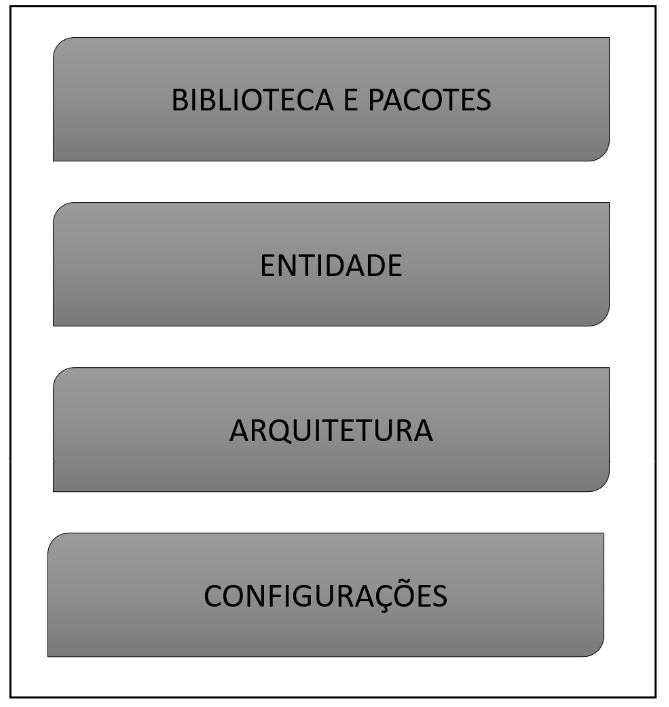
\includegraphics[scale=0.37]{figuras/ESTR_VHDL.png}\\
    {\footnotesize Fonte: Autoria própria.}
    \label{fig:vhdl_blocos}
\end{figure}

A interface define os sinais lógicos de entrada e saída do circuito projetado. O bloco de arquitetura descreve a operação interna do design. Dentro desses blocos, existem vários outros blocos funcionais usados para construir os elementos de design do circuito lógico sendo criado. Após a criação do projeto, ele pode ser simulado e sintetizado para verificar seu funcionamento lógico \cite{ordonez2003projeto}. A estrutura de uma descrição VHDL é mostrado na figura \ref{fig:vhdl_blocos_estrut}.

\begin{figure}[!htb]
    \centering
    \caption{A estrutura de uma descrição VHDL com os seus blocos}
    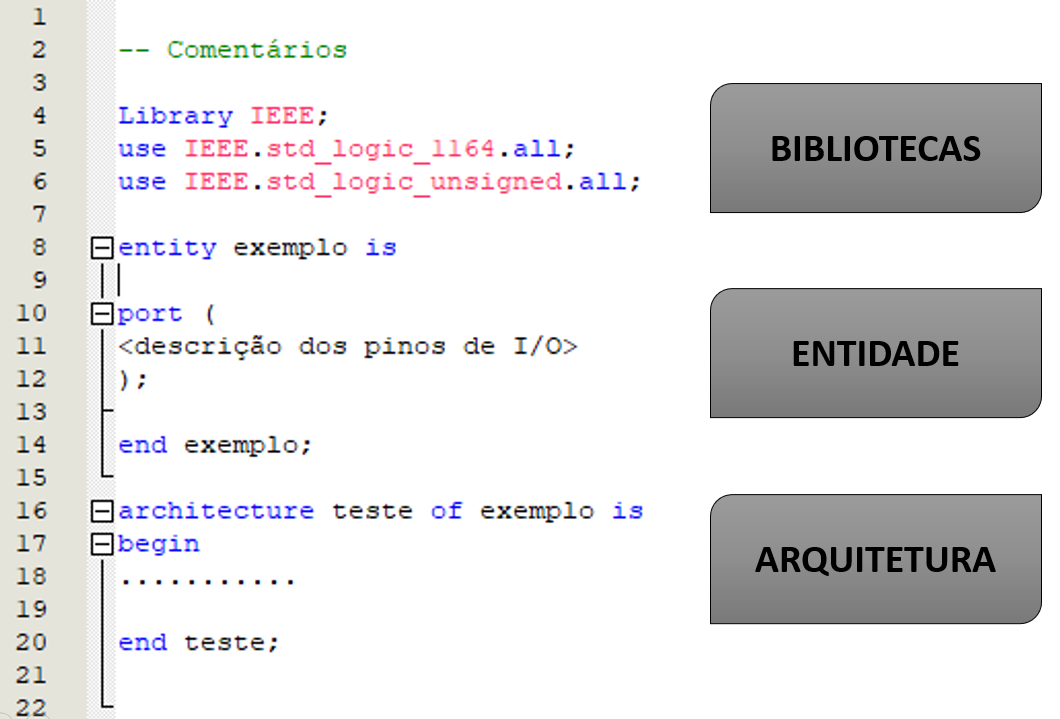
\includegraphics[height = 9cm]{figuras/estrut_blocVHDL.png}\\
    {\footnotesize Fonte: Autoria própria.}
    \label{fig:vhdl_blocos_estrut}
\end{figure}
 
\subsubsection{Declaração de biblioteca e Pacotes}

As bibliotecas e os pacotes são conjuntos de declarações usadas para um determinado fim. Pode ser um conjunto de subprogramas, ou funções que operem com um tipo de dado, assim como pode ser um conjunto de declarações necessárias para modelar um determinado projeto. Uma biblioteca é usada para organizar e gerenciar diferentes unidades de design em um projeto VHDL. É comum criar diferentes bibliotecas para organizar e armazenar unidades de design relacionadas. Por exemplo, uma biblioteca pode ser criada para armazenar unidades de design relacionadas a interface serial, enquanto outra biblioteca pode ser criada para armazenar unidades de design relacionadas a processamento de sinais \cite{roth2004circuit}.

Os pacotes são usados para definir e compartilhar constantes, tipos de dados, funções, procedimentos e outras construções que podem ser usadas em várias unidades de design. Os pacotes podem ser usados para evitar a repetição de código e facilitar a reutilização de código em diferentes unidades de design \cite{ordonez2003projeto}. Por exemplo, um pacote pode ser criado para definir um tipo de dado personalizado que é usado em várias unidades de design. 
Bibliotecas e Pacotes mais utilizados estão citados no quadro \ref{quadro_1}.
%+++++++++++++++++++++++++++++++++++++++++++++++

\begin{quadro}[h]
    \caption{Pacotes mais utilizados (Biblioteca IEEE)}
    \label{quadro_1}
    \centering
     \begin{tabular}{|c|p{3cm}|p{8cm}|}
      \hline
      \textbf{Pacote} & \textbf{Tipos de dados} & \textbf{Descrição} \\
      \hline
      std\_logic & std\_logic e std\_logic\_vector & Define o padrão para descrever a interconexão entre tipos de dados usados na linguagem VHDL \\
      \hline
       std\_logic\_arith & Especifica tipos de dados sinalizados e não sinalizados & Funções de conversão, operações aritméticas e comparações para uso de dados sinalizados e não sinalizados \\
      \hline
       std\_logic\_unsigned & std\_logic\_vector & Define funções que permitem usar tipos de dados std\_logic\_vector, como se fossem tipo de dado não sinalizado \\
      \hline
       std\_logic\_signed & std\_logic\_vector & Define funções que permitem usar tipos de dados std\_logic\_vector, como se fossem tipo de dado sinalizado \\
      \hline
       numeric\_std & & Substitui os pacotes usados juntos std\_logic\_atith, std\_logic\_unsigned e std\_logic\_signed \\
      \hline                 
    \end{tabular}
  \vspace{1.5pt}
  \caption*{\footnotesize Fonte: \cite{ordonez2003projeto}}
\end{quadro}

A declaração do uso de pacotes e bibliotecas é mostrada no quadro \ref{quadro_2}. O uso de .all implica que todos os elementos da biblioteca podem ser usados.

\subsubsection{Declaração de Entidade}

Modelo de tabela:

\begin{table}[htb]
\ABNTEXfontereduzida
\center \caption{Parâmetros da Condutividade Intrabanda do Grafeno \cite{b5}\cite{b13}}
\label{Tab}
\begin{tabular}{p{0.6cm} p{2cm} p{2cm} p{6cm}}
  \hline
   \textbf{ } & \textbf{Valor}  & \textbf{Unidade}  & \textbf{Descrição}  \\[1.5pt]
   	\hline
$e$  &  $1,60\times10^{-19}$  &   $C$  &    Carga do Elétron\\[1.5pt]
$\hbar$   &   $1,05\times10^{-34}$ & $J\!\cdot\!s/rad $ & Constante de Plank Reduzida\\[1.5pt]
$k_B$   &   $1,38\times10^{-23}$ & $J/K $ & Constante de Boltzmanm\\[1.5pt]
$T$   &   $300$ & $K$ &  Temperatura\\
$\sigma_0$   &   $e^2/4\hbar$ & $S\!\cdot\!rad$ & Condutividade HF\\[1.5pt]
$\mu_c$   &   $0; 0,25; 0,5$ & $eV$ & Potencial Químico\\[1.5pt]
$\tau$   &   $0,5$ & $ps$ & Tempo de Amortecimento\\[1.5pt]
\hline
\end{tabular}  
  \vspace{1.5pt}
  \caption*{\footnotesize Fonte: \cite{ordonez2003projeto}}
\end{table}

Primeiramente, para modo TE ( Fig. \ref{Fig9}a), os campos elétrico e magnético no meio 1 são compostos pela onda incidente e pela onda refletida, de forma que:
\begin{equation}\label{eq3.2}
\textbf{E}_1(x,z) = -\hat{a}_y\left[E_{iy}e^{-jk_{z1}(z+d_1)} + E_{ry}e^{+jk_{z1}(z+d_1)}\right]e^{-jk_x x}  
\end{equation}
\begin{equation}\label{eq3.3}
\begin{split}
\textbf{H}_1(x,z) = \hat{a}_x\left[H_{ix}e^{-jk_{z1}(z+d_1)} - H_{rx}e^{+jk_{z1}(z+d_1)}\right]e^{-jk_x x} \qquad\qquad
\\
-\hat{a}_z\left[H_{iz}e^{-jk_{z1}(z+d_1)} + H_{rz}e^{+jk_{z1}(z+d_1)}\right]e^{-jk_x x} 
\end{split}
\end{equation}

\noindent onde $E_{iy}$, $H_{ix}$ e $H_{iz}$ são as amplitudes dos campos EH que compõem a onda incidente, e $E_{ry}$, $H_{rx}$ e $H_{rz}$ são as amplitudes dos campos EH que compõem a onda refletida.
\begin{equation}\label{eq3.2}
\textbf{E}_1(x,z) = -\hat{a}_y\left[E_{iy}e^{-jk_{z1}(z+d_1)} + E_{ry}e^{+jk_{z1}(z+d_1)}\right]e^{-jk_x x}  
\end{equation}
\chapter{Desenvolvimento}
\label{cap_desenvolvimento}

%\section{ Descrição do Sistema}
%teste
teste
teste
teste


\section{Aeropêndulo}
Os sistemas mecânicos têm como uma de suas característica os graus liberdade, o Aeropêndulo tem um grau de liberdade, sendo o ângulo $\theta$, assim o sistema tem apenas uma variável a ser controlada a partir do empuxo gerado pelas hélices, que por sua vez depende da velocidade angular do eixo do motor CC Série acoplado ao braço do Aeropêndulo. Dessa forma, podemos analisar o sistema a partir da entrada e da saída, sendo a entrada a tensão no motor e a saída o ângulo $\theta$ do braço do Aeropêndulo.

\begin{figure}[!h]
	\centering
	\caption{Diagrama esquemático do Aeropêndulo.}
	\efbox{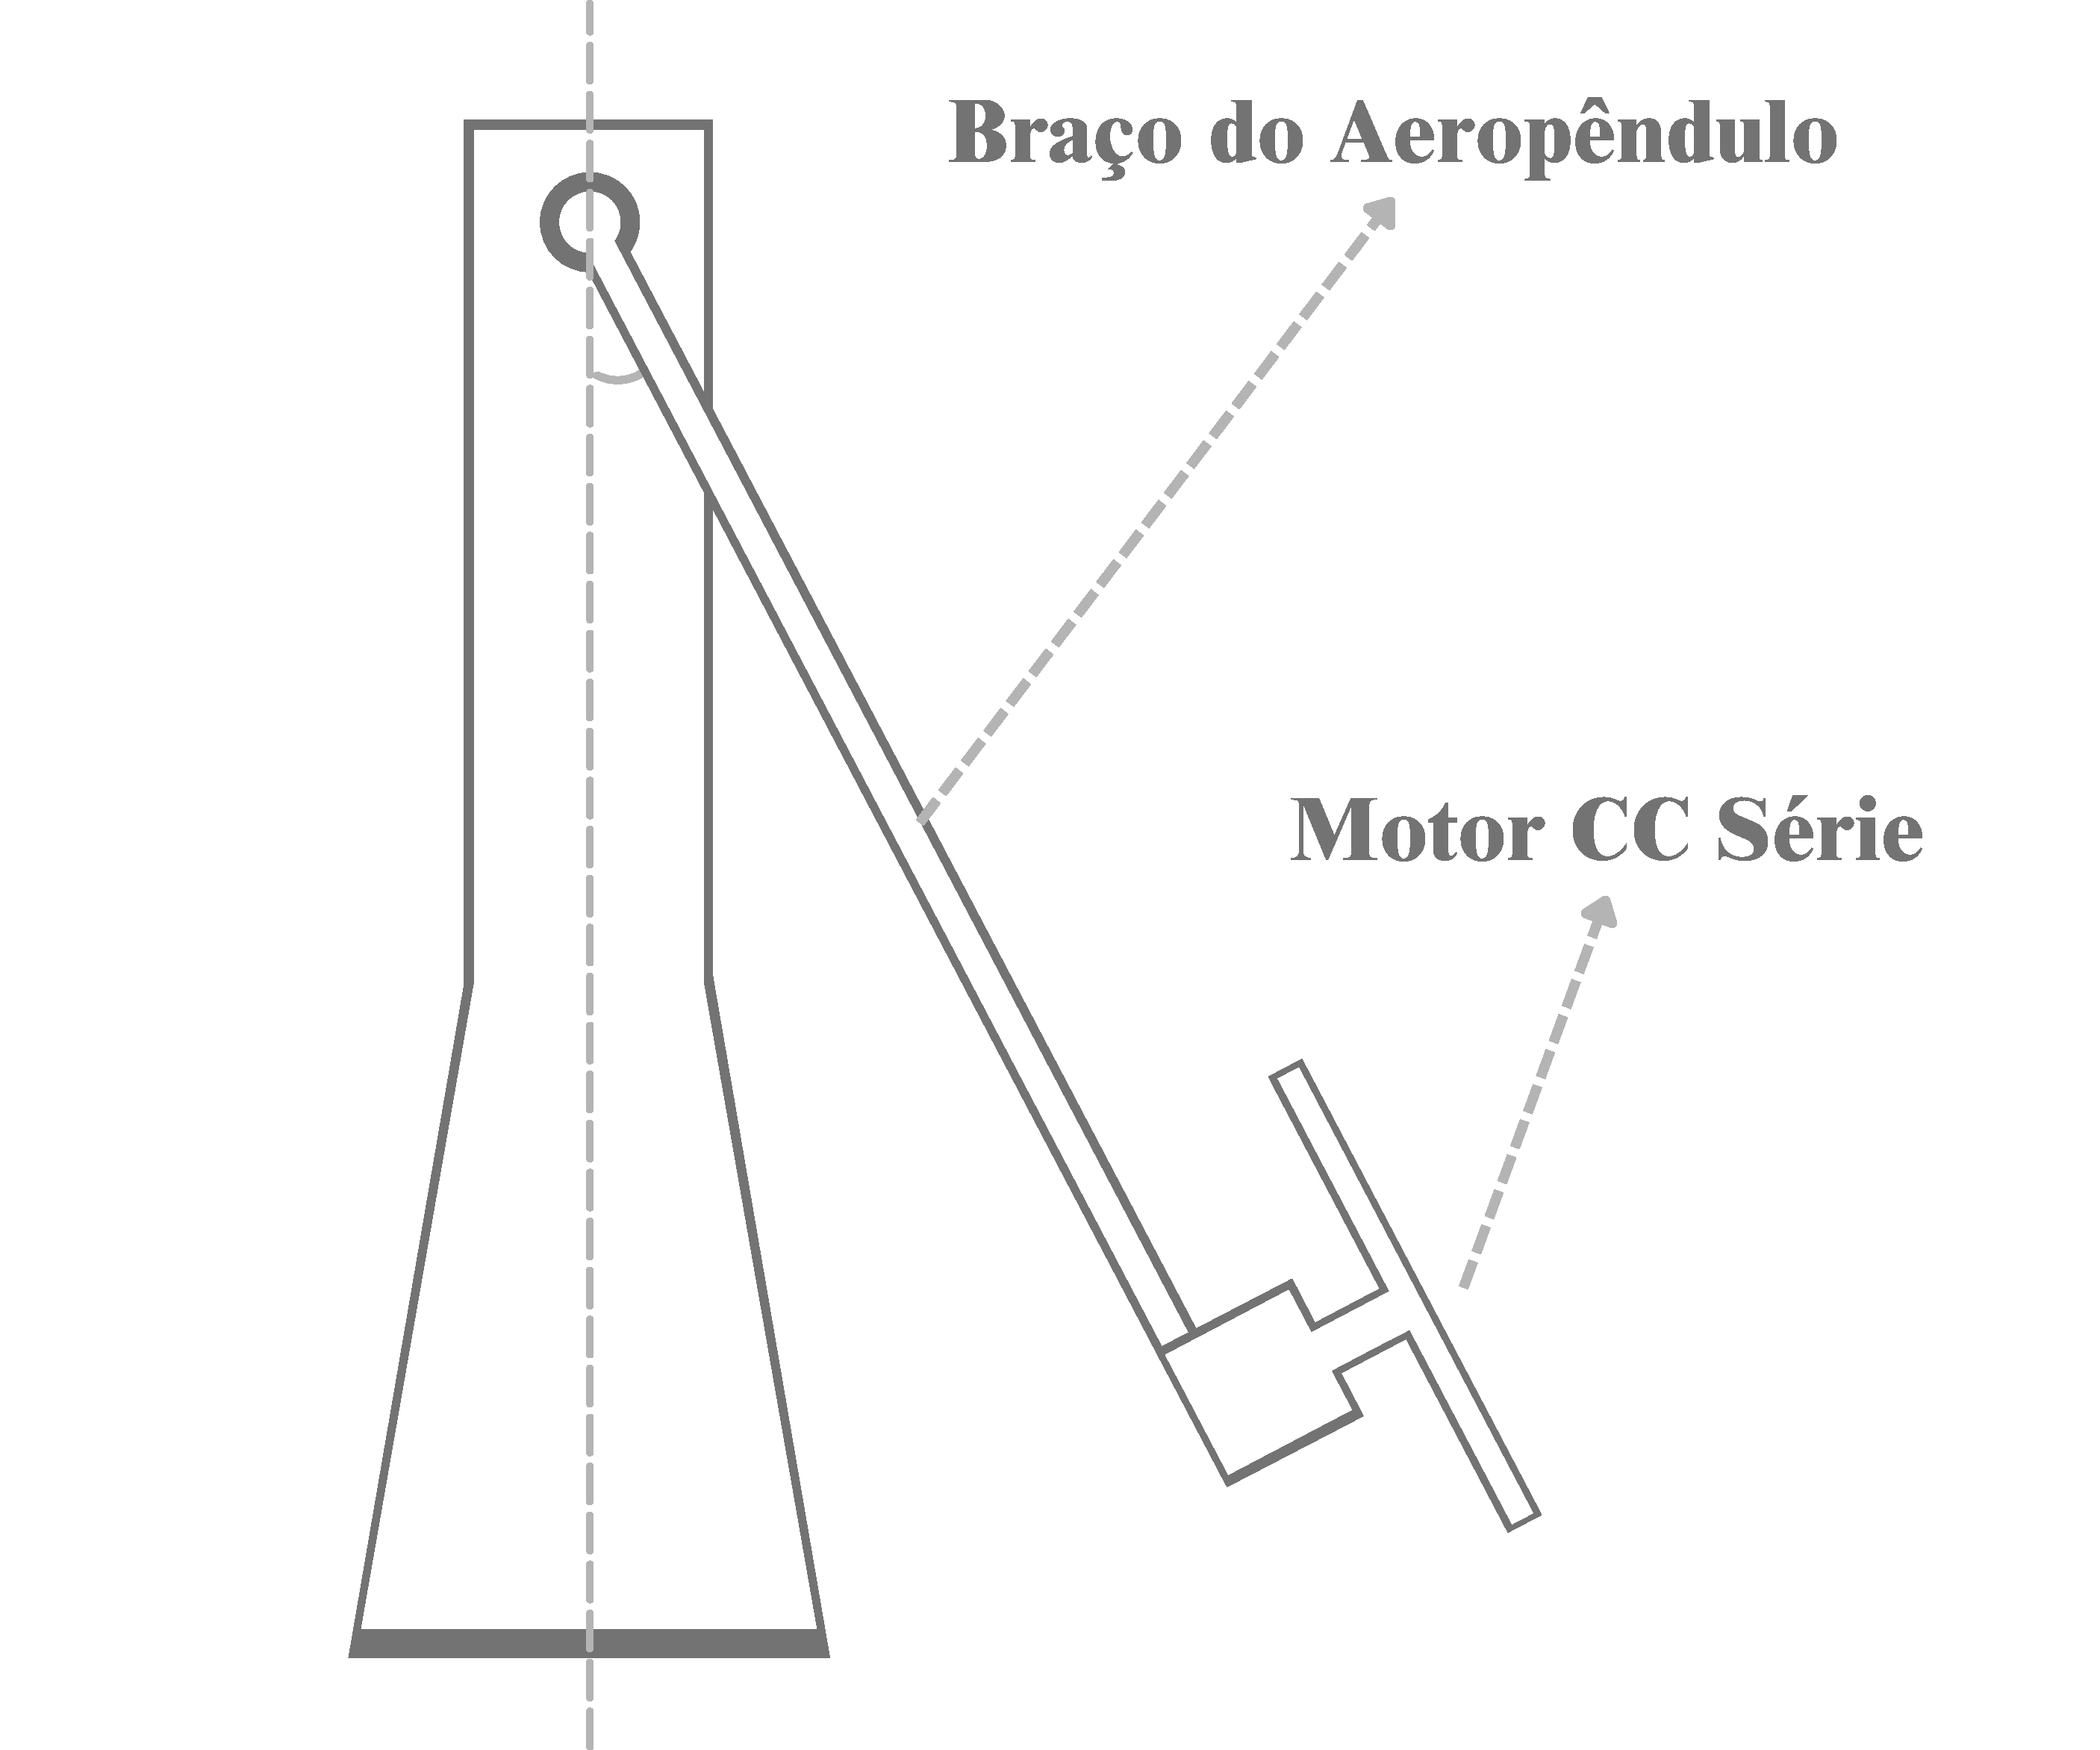
\includegraphics[width=0.55\textwidth]{Capitulos/2_aeropendulo/4_figuras/diagrama_aeropendulo_01.pdf}}
	\caption*{Fonte: elaborado pelo autor (2023).}
        \label{fig4:image_04}
\end{figure}




\section{ Fundamentação Teórica}
\label{fundamentacao_teorica}

O processo que envolve modelagem de sistemas físicos em termos de equações matemáticas é uma das partes mais importante no estudo de sistemas de controle. Segundo \citeonline[p.~11]{ogata5ed}, o modelo matemático de um sistema dinâmico é definido como um conjunto de equações que representa a dinâmica do sistema com precisão ou, pelo menos, razoavelmente bem.

A construção de modelos matemáticos adequados é fundamental na análise de sistemas de controle, pois a dinâmica de diversos sistemas, como mecânicos, elétricos, térmicos, econômicos, biológicos, entre outros, pode ser expressa por meio de equações diferenciais. Tais equações são derivadas das leis físicas que governam cada sistema específico, como as leis de Newton para sistemas mecânicos e as leis de Kirchhoff para sistemas elétricos. Esta abordagem ressalta a importância crucial de compreender as bases matemáticas subjacentes para uma análise abrangente dos sistemas de controle, conforme destacado por \citeonline[p.~11]{ogata5ed}.


% \section{Modelagem Analítica}

Para realizar a modelagem do Aeropêndulo pode-se aplicar diferentes métodos, uma abordagem inicial para modelar sistemas físicos consiste em empregar as leis fundamentais da física. Além disso, em situações mais complexas, é viável decompor o sistema em subsistemas menores e, em seguida, desenvolver modelos para cada um deles. Por fim, é possível conectar esses modelos, de forma a obter uma representação aproximada do sistema real. Dessa maneira, podemos obter uma compreensão mais aprofundada e abrangente da dinâmica do sistema em questão. A figura \ref{fig4:image_01} mostra um diagrama da representação do Aeropêndulo como um conjunto de subsistemas.


\begin{figure}[!h]
	\centering
	\caption{Subsistemas do  Aeropêndulo.}
            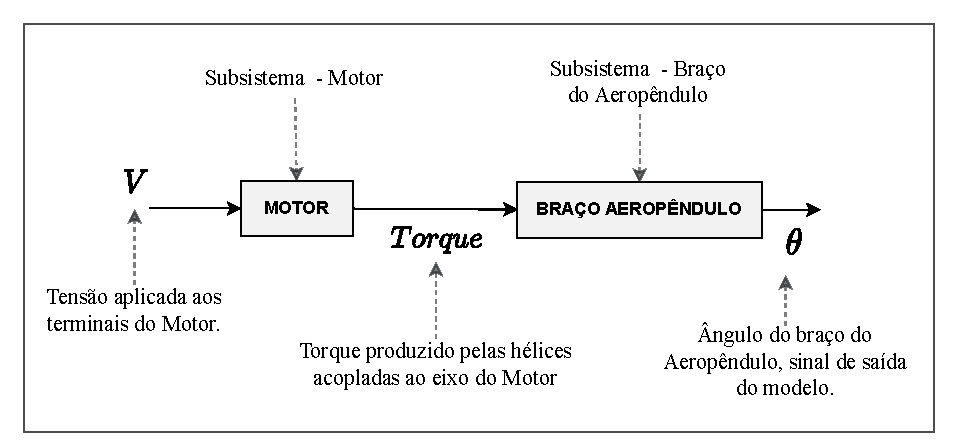
\includegraphics[width=0.9\textwidth]{Capitulos/2_aeropendulo/4_figuras/subsistemas_aeropendulo.pdf}
	\caption*{Fonte: elaborado pelo autor (2023).}
        \label{fig4:image_01}
\end{figure}



\newpage

\subsection{ Modelo Matemático Braço do Aeropêndulo}
\label{modelagem_braco_aeropendulo}

Como previamente abordado, é possível segmentar o sistema em dois subsistemas distintos: o motor CC Série e o braço do Aeropêndulo. Nesta seção, o foco estará concentrado na modelagem do braço do Aeropêndulo, utilizando como referência o trabalho de \cite{amin} para a obtenção da equação que descreve a dinâmica desse componente.


\begin{figure}[!h]
	\centering
	\caption{Diagrama esquemático do Braço do Aeropêndulo.}
	\efbox{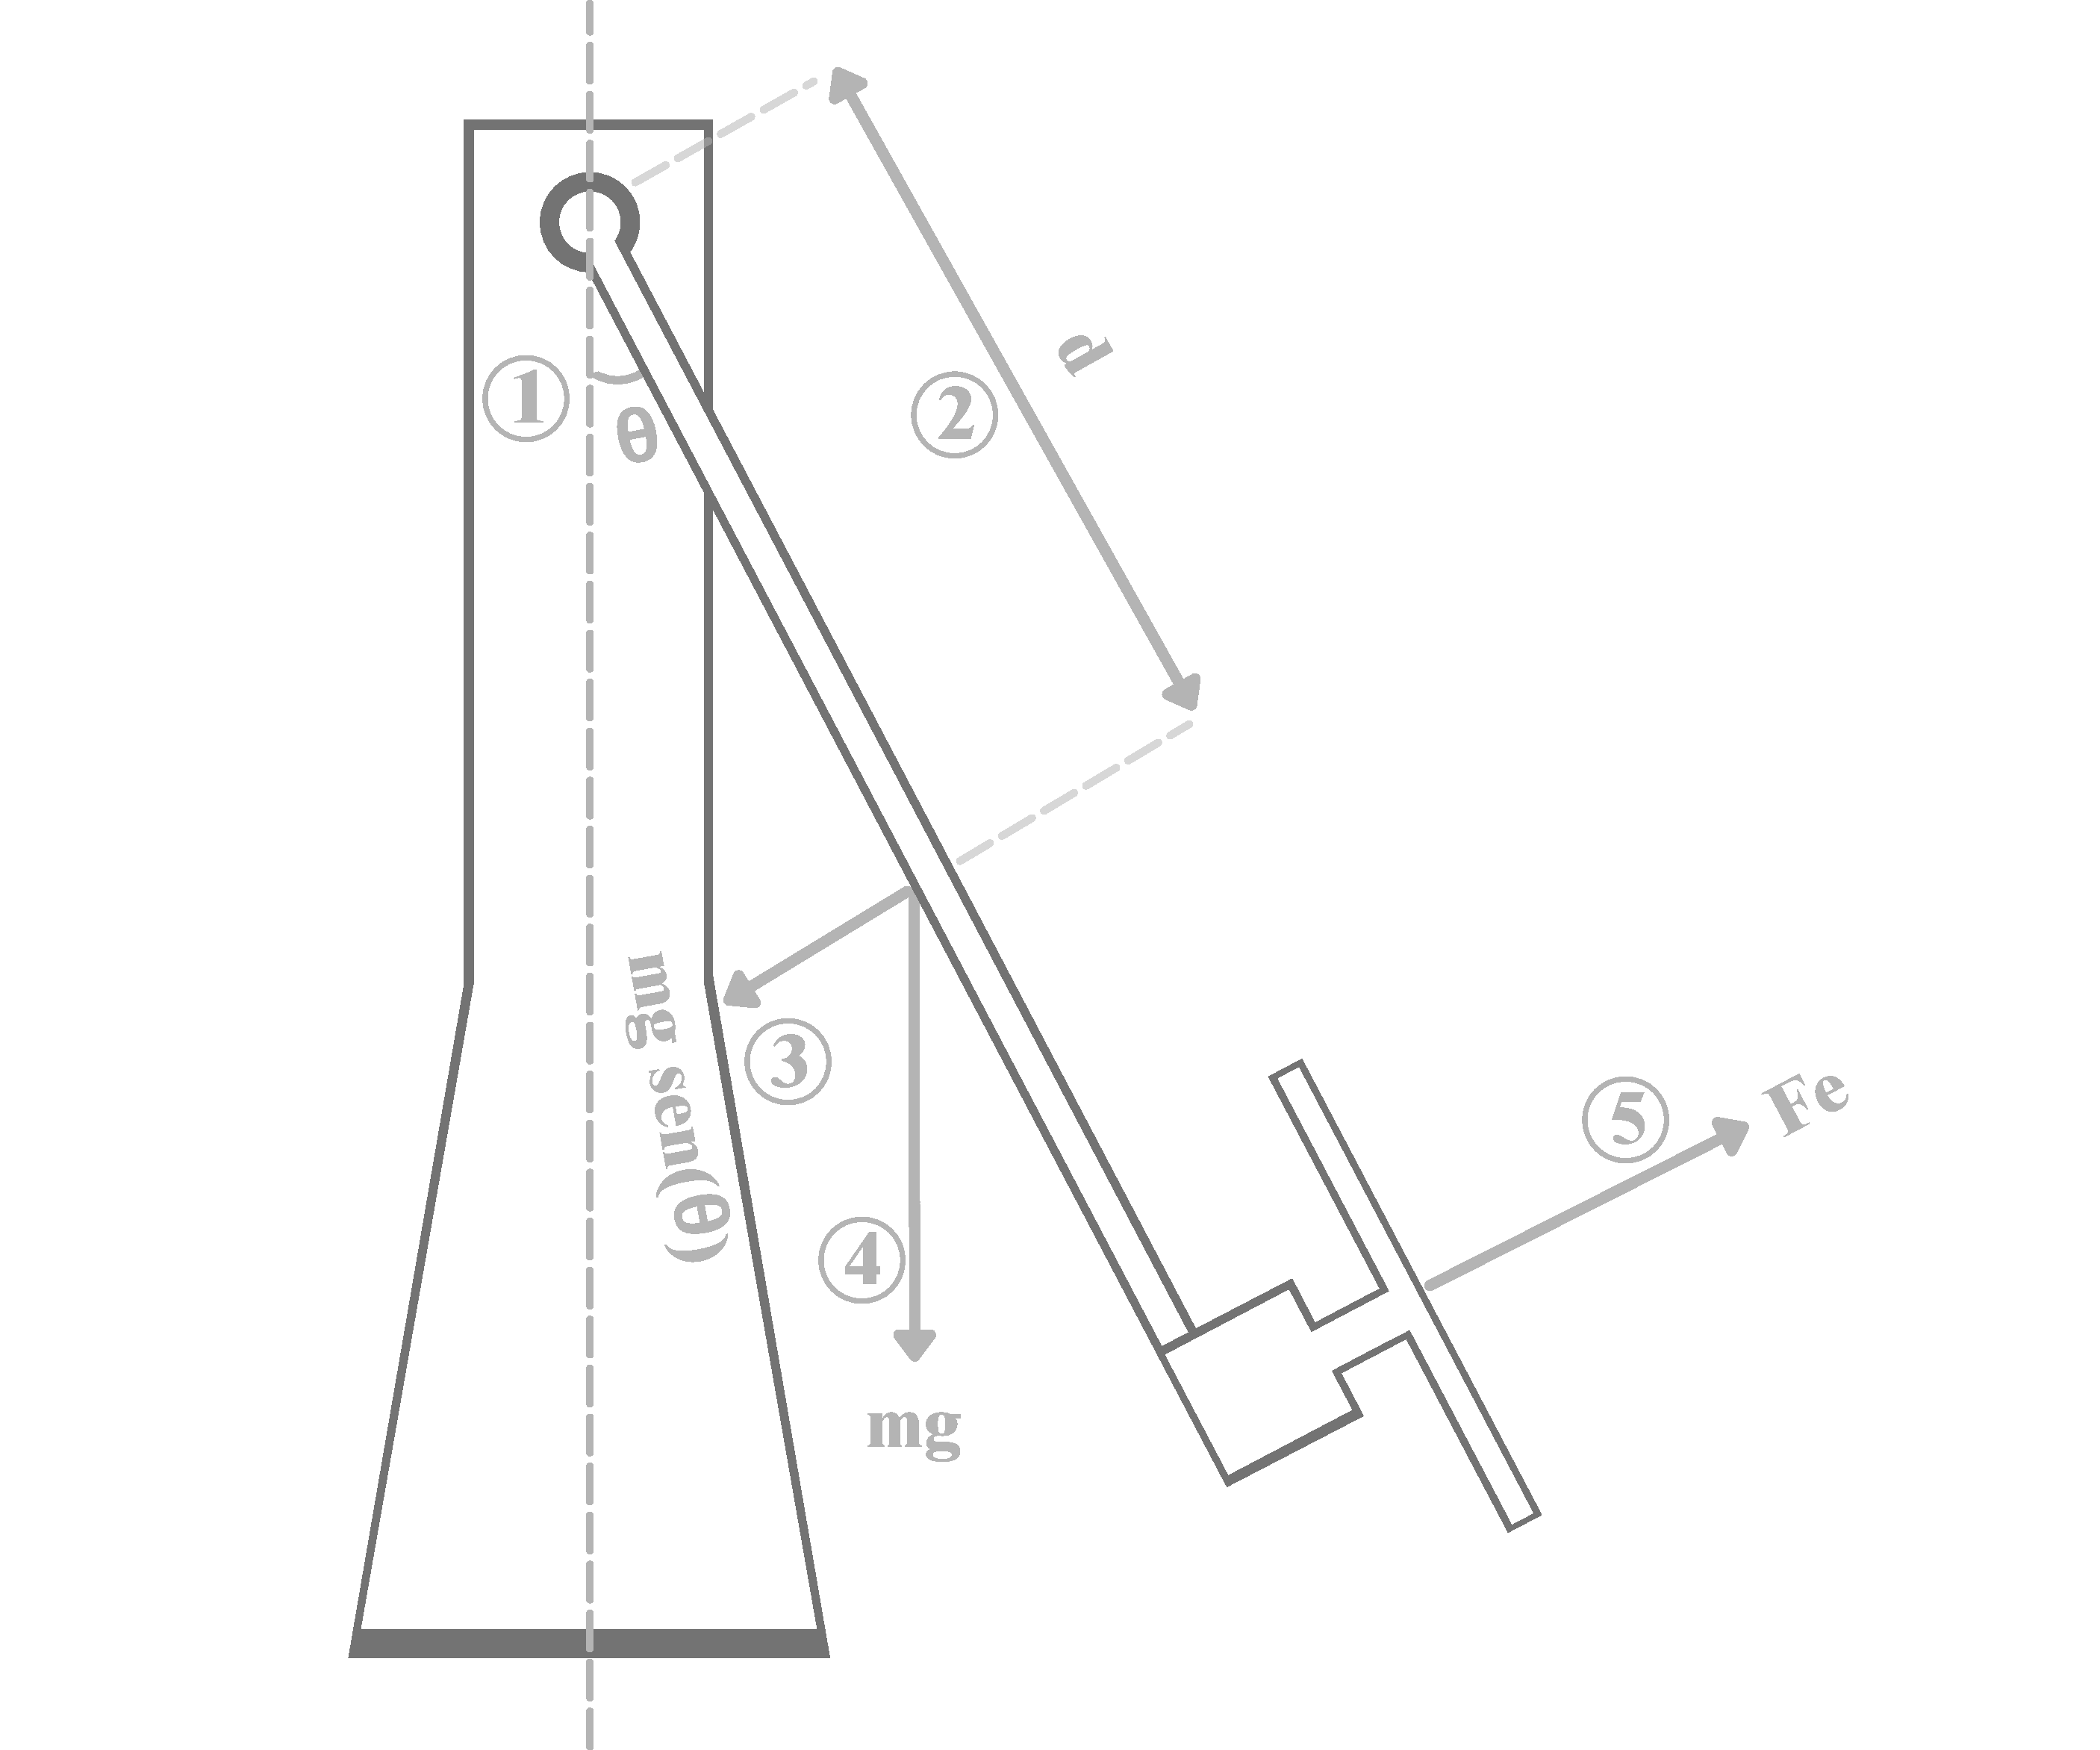
\includegraphics[width=0.55\textwidth]{Capitulos/2_aeropendulo/4_figuras/desenho_aeropendulo.pdf}}
	\caption*{Fonte: elaborado pelo autor (2023).}
        \label{fig4:image_04}
\end{figure}


O modelo matemático do braço do Aeropêndulo é derivado a partir das leis de Newton e do momento angular, como mostra \cite{amin}. assim, se obtém a equação \ref{eq4:eq38}.

\begin{align}
    F_e &= J_b\ddot{\theta} + c\dot{\theta} +mgd\sin{\theta}  \label{eq4:eq38}
\end{align}

\noindent Onde:

\begin{itemize}
        \setlength{\itemsep}{-2pt}
	\item  $F_e$: Empuxo gerado pela hélice
        \item  $J_b$: Momento de inércia do Braço
        \item  $\theta$: posição angular do Aeropêndulo
        \item  $c$: coeficiente de amortecimento viscoso
        \item  $m$: massa do Aeropêndulo
        \item  $d$: a distância entre o centro de massa e o ponto de pivô
\end{itemize}

A entrada do subsistema do braço do Aeropêndulo é a força de empuxo proporcionada pela hélice, porém, o modelo do motor CC Série tem como saída a velocidade angular, dessa forma é preciso encontrar uma relação entre a velocidade $\omega$ e o empuxo $F_e$, essa relação é não linear, $F_e = K_m\omega^2$, porém é possível aproximar por uma relação linear,  $F_e = K_m\omega$, em que $K_m$ é um ganho que relaciona a velocidade angular com o empuxo. Com isso, pode-se relacionar a velocidade angular $\omega$  com o empuxo $F_e$ gerado pela hélice do Aeropêndulo.

O modelo encontrado tem uma parcela não linear dada por $\sin{\theta}$, para aplicar técnicas de projeto de controle é preciso obter o modelo linearizado da planta, isso pode ser feito considerando $\sin{\theta} \approx \theta$ para pequenas variações em torno de $\theta$. dessa forma, temos a seguinte linearização:
\begin{align}
    F_e &= J_b\ddot{\theta} + c\dot{\theta} +mgd\theta
    \label{eq4:eq39}
\end{align}

Aplicando a transformada de Laplace para encontrar a função de transferência do subsistema, tem-se:

\begin{align}
    F_e(s) &= J_b\theta(s)s^2 + c\theta(s)s + mgd\theta(s) \label{eq4:eq41}\\
    F_e(s) &= (J_bs^2 + cs +mgd)\theta(s) \label{eq4:eq42}\\
    \dfrac{\theta(s)}{F_e(s)} &= \frac{1}{J_bs^2 + cs + mgd} \label{eq4:eq43}
\end{align}


Agora que foi obtido o modelo do braço do Aeropêndulo, pode-se usar a relação linearizada $F_e = K_m\omega$ para usar a saída do modelo do motor cc série como entrada do modelo do braço do Aeropêndulo, como mostrado na equação \ref{eq4:eq46}.

\begin{align}
    \dfrac{\theta(s)}{K_m\omega(s)} &= \dfrac{1}{J_bs^2 + cs +mgd} \label{eq4:eq44}\\
    \dfrac{\theta(s)}{\omega(s)} &= \dfrac{K_m}{J_bs^2 + cs +mgd} \label{eq4:eq45}\\
    H(s) = \dfrac{\theta(s)}{\omega(s)} &= \dfrac{\dfrac{K_m}{J_b}}{s^2 + \dfrac{c}{J_b}s +\dfrac{mgd}{J_b}} \label{eq4:eq46}
\end{align}


A equação \ref{eq4:eq46} representa a função de transferência que descreve o comportamento dinâmico do braço do Aeropêndulo. Esta expressão matemática encapsula as relações fundamentais entre as variáveis de entrada/saída do sistema, oferecendo uma visão abrangente e quantitativa da resposta do braço às diferentes condições e estímulos. Ao analisar a função de transferência, podemos compreender como as mudanças nas entradas afetam as saídas.


\subsection{Modelo Matemático do Motor CC Série}
\label{modelagem_motorccserie}

Os motores CC série tem como principal característica possuir o enrolamento de campo em série com o enrolamento de armadora, essa configuração resulta em um motor com torque de partida alto, porém, o torque reduz a medida que a velocidade aumenta devido ao aumento da Força Eletromotriz FEM. Por conta desse aumento de FEM os motores CC Séries tem uma regulação de velocidade ruim, quando se aumenta a carga no eixo do motor a velocidade é reduzida que por sua vez reduz a FEM e então o torque aumenta para conseguir atuar na carga.


No contexto dos motores série, observamos que o aumento da carga resulta em incrementos na corrente, na Força Magnetomotriz (FMM) da armadura e no fluxo do campo do estator, contanto que o ferro não atinja a saturação completa. À medida que o fluxo aumenta com a carga, a velocidade do motor série deve diminuir para manter um equilíbrio adequado entre a tensão aplicada e a força contraeletromotriz. Além disso, o aumento na corrente de armadura, ocasionado pelo acréscimo no conjugado, é menor em comparação com o motor em derivação, devido ao aumento no fluxo. Dessa forma, o motor série é caracterizado como um motor de velocidade variável \citeonline[p.~410]{umans2014}.


No entanto, mesmo motores cc série com dimensões reduzidas geram torques altos com baixo consumo de corrente. Visando melhorar seu desempenho, é possível projetar controladores de malha fechada capazes de tornar esses motores mais eficientes na regulação de velocidade.

Para realizar a modelagem o motor CC série, foi usado a base teórica de \cite{jesus}, A figura \ref{fig4:image_02} mostra um diagrama da configuração do motor CC Série, no qual o enrolamento de campo está conectado em série com o enrolamento de armadura, dessa forma, a  corrente de campo é igual a corrente de armadura $ i = i_f = i_a$.


\begin{figure}[!h]
	\centering
	\caption{Motor CC Série.}
	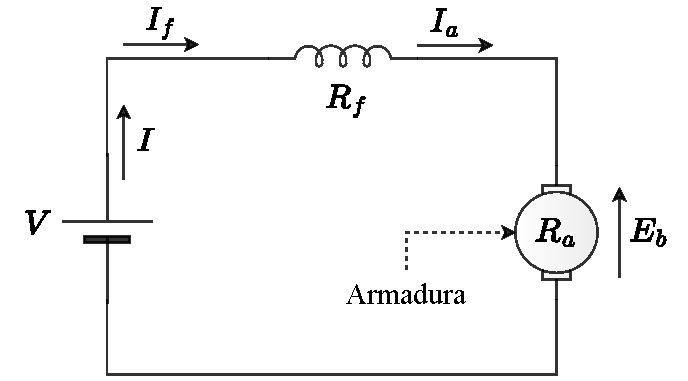
\includegraphics[width=0.7\textwidth]{Capitulos/2_aeropendulo/4_figuras/esquema_motor_cc.pdf}
	\caption*{Fonte:  elaborado pelo autor (2023).}
	\label{fig4:image_02}
\end{figure}

Na figura \ref{fig4:image_03}, mostra o diagrama eletromecânico do motor, nele pode-se observar que os componentes elétricos estão todos em série, no qual o enrolamento de campo possui uma parte resistiva e outra indutiva, assim como o enrolamento de armadura, já a parte mecânica possui uma velocidade angular dada por $\omega$, torque eletromagnético do motor dado por $T_e$ e torque da Carga $T_c$.


\begin{figure}[!h]
	\centering
	\caption{Diagrama Elétrico/Mecânico Motor CC Série.}
	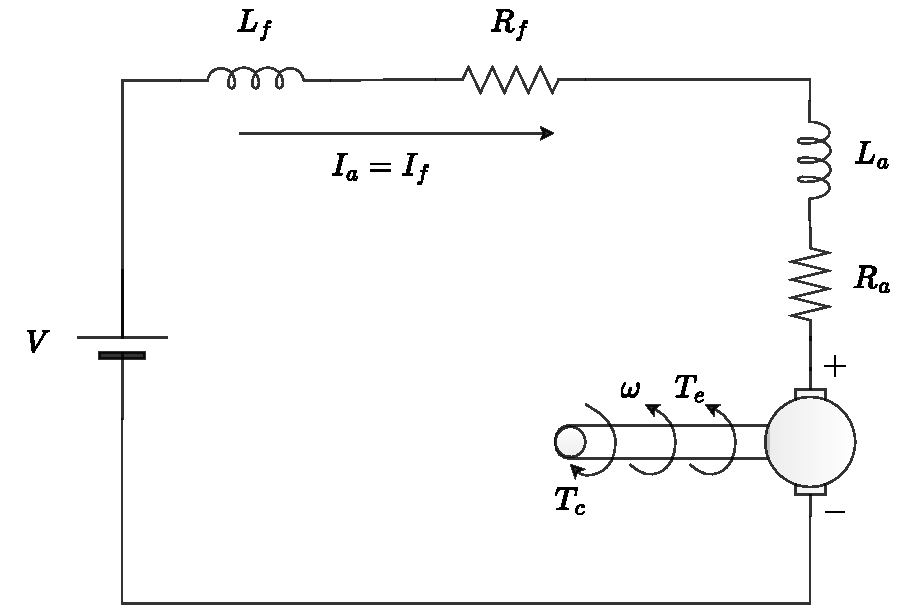
\includegraphics[width=0.6\textwidth]{Capitulos/2_aeropendulo/4_figuras/diagrama_motor_cc.pdf}
	\caption*{Fonte: elaborado pelo autor (2023).}
	\label{fig4:image_03}
\end{figure}


%%%%%%%%%%%%%%%%%%%%%%%%%%%%%%%%%%%%%%%%%%%%%%%%%%%%%%%%%%%%%%%%%%%%%%%%%%%%%%%%%%%%%%%%%%%%%%%%%%%%%%%%%%%%%%%%%%%%%%%%%%%%%%%%%%%%%%%%%
%%%%%%%%%%%%%%%%%%%%%%%%%%%%%%%%%%%%%%%%%%%%% Modelagem da Parte Mecânica do Motor CC Série %%%%%%%%%%%%%%%%%%%%%%%%%%%%%%%%%%%%%%%%%%%%%
%%%%%%%%%%%%%%%%%%%%%%%%%%%%%%%%%%%%%%%%%%%%%%%%%%%%%%%%%%%%%%%%%%%%%%%%%%%%%%%%%%%%%%%%%%%%%%%%%%%%%%%%%%%%%%%%%%%%%%%%%%%%%%%%%%%%%%%%%

%\subsubsection{Modelagem da Parte Mecânica do Motor CC Série}

Primeiramente a parte mecânica do motor será modelada, um motor cc série é composto por uma parte rotativa "armadura", de modo que, essa parte, gera um momento de inércia $J_m$ no eixo do motor e um fator de amortecimento viscoso $b$, além disso, o eixo possui uma velocidade angular $\dot{\omega}$.

Assim, a equação \ref{eq4:eq1}, obtida a partir de \cite{jesus}, descreve o modelo mecânico do motor CC Série.

\begin{align}
	J_m\ddot{\omega}(t) &= T_e(t) - b\dot{\omega}(t) - T_c(t) \label{eq4:eq1}
\end{align}


Ao expressar o torque $T_e(t)$ em função das outras variáveis, obtém-se a equação \ref{eq4:eq2}.

\begin{align}
	T_e(t) &= J_m\ddot{\omega}(t) + b\dot{\omega}(t) + T_c(t) \label{eq4:eq2}
\end{align}


\noindent Onde:
\begin{itemize}
        \setlength{\itemsep}{-2pt}
	\item $T_e$: Torque Eletromagnético produzido pelo Motor;
	\item $J_m$: Momento de Inércia do Eixo do Motor;
	\item $\ddot{\omega}$: Aceleração Angular do Eixo do Motor;
	\item $\dot{\omega}$: Velocidade Angular do Eixo do Motor;
	\item $b$: Fator de Amortecimento Viscoso;
	\item $T_c$: Torque de Carga.
\end{itemize}

Tanto a Força Eletromotriz $E_A(t)$ quanto o Torque Eletromagnético $T_e(t)$ dependem do fluxo magnético do entreferro $\Phi$, com isso, tem-se as equações \ref{eq4:eq3} e \ref{eq4:eq4}.

\begin{align}
	E_a(t) &= \dot{\omega}(t) \Phi{(i)} \label{eq4:eq3}\\
	T_e(t) &= i(t) \Phi{(i)}			\label{eq4:eq4}
\end{align}

O Fluxo magnético depende da corrente $i(t)$, assim, as equações \ref{eq4:eq1} e \ref{eq4:eq2} são não-lineares. Além disso, pode-se aproximar o fluxo $\Phi$ por uma relação linear, $K_0$, ao desprezar a saturação magnética.

\begin{align}
	\Phi(i) &= K_0 i(t) \label{eq4:eq5}
\end{align}

A constante $K_0$ é a indutância mútua entre a armadura e o enrolamento de campo. Agora pode-se encontrar o modelo não-linear da parte mecânica do Motor CC Série, substituindo \ref{eq4:eq5} em \ref{eq4:eq4}, obtém-se a expressão \ref{eq4:eq7}:

\begin{align}
	T_e(t) &= i(t) K_0 i(t) \label{eq4:eq6}\\
	T_e(t) &= K_0 i^2(t) 	\label{eq4:eq7}
\end{align}

Substituindo \ref{eq4:eq7} em \ref{eq4:eq2}, é possível encontrar o modelo da parte mecânica do motor CC série, assim, tem-se a expressão  \ref{eq4:eq8}.


\begin{align}
	K_0 i^2(t) &= J_m\ddot{\omega}(t) + b\dot{\omega}(t) + T_c(t) \label{eq4:eq8}
\end{align}


%%%%%%%%%%%%%%%%%%%%%%%%%%%%%%%%%%%%%%%%%%%%%%%%%%%%%%%%%%%%%%%%%%%%%%%%%%%%%%%%%%%%%%%%%%%%%%%%%%%%%%%%%%%%%%%%%%%%%%%%%%%%%%%%%%%%%%%%%
%%%%%%%%%%%%%%%%%%%%%%%%%%%%%%%%%%%%%%%%%%%%% Modelagem da Parte Elétrica do Motor CC Série %%%%%%%%%%%%%%%%%%%%%%%%%%%%%%%%%%%%%%%%%%%%%
%%%%%%%%%%%%%%%%%%%%%%%%%%%%%%%%%%%%%%%%%%%%%%%%%%%%%%%%%%%%%%%%%%%%%%%%%%%%%%%%%%%%%%%%%%%%%%%%%%%%%%%%%%%%%%%%%%%%%%%%%%%%%%%%%%%%%%%%%

% \subsubsection{Modelagem da Parte Elétrica do Motor CC Série}

Para a parte elétrica, utilizou-se a lei de Kirchhoff das tensões para modelar o sistema. assim como a parte mecânica, o modelo da parte elétrica foi baseado de \cite{jesus}, o motor em questão é um motor de corrente contínua CC série, Dessa forma, $i_a = i_f$, portanto, obtém-se a expressão \ref{eq4:eq9}.


\begin{align}
	V(t) &= (R_a + R_f)i(t)+ (L_a + L_f)\dfrac{d}{dt}i(t) + E_a \label{eq4:eq9}
\end{align}

\noindent Onde:

\begin{itemize}
        \setlength{\itemsep}{-2pt}
	\item $V$: Tensão da Fonte;
	\item $R_a$: Resistência da Armadura;
	\item $R_f$: Resistência de Campo;
	\item $i_a$: Corrente da Armadura;
	\item $i_f$: Corrente de Campo;
	\item $E_A$: Tensão Contro Eletromotriz Gerada pela Armadura;
	\item $L_a$: Impedância da Armadura;
	\item $L_f$: Impedância de Campo.
\end{itemize}

Como os componentes elétricos então em série, pode-se obter uma resistência total assim como uma indutância:

\begin{align}
	R &= R_a + R_f          \label{eq4:eq10}\\        
	L &= L_a + L_f          \label{eq4:eq11}
\end{align}

\begin{align}
	V(t) &= Ri(t)+ L\dfrac{d}{dt}i(t) + E_a \label{eq4:eq12}
\end{align}

Substituindo \ref{eq4:eq5} em \ref{eq4:eq3}, obtém-se a equação \ref{eq4:eq13}.

\begin{align}
	E_a(t) &= \dot{\omega}(t)K_0 i(t) \label{eq4:eq13}
\end{align}

Por fim, pode-se encontrar a equação que descreve a parte elétrica do sistema ao substituir \ref{eq4:eq13} em \ref{eq4:eq12}, assim, obtendo a equação \ref{eq4:eq14}.

\begin{align}
	V(t) &= Ri(t)+ L\frac{d}{dt}i(t) + \dot{\omega}(t)K_0 i(t) \label{eq4:eq14}
\end{align}

Dessa forma, as equações que modelam um Motor CC série são expressas por \ref{eq4:eq15} e \ref{eq4:eq16}, em que \ref{eq4:eq15} esta relacionada a parte mecânica e \ref{eq4:eq16} a parte elétrica.

\begin{align}
	K_0 i^2(t) &= J_m\ddot{\omega}(t) + b\dot{\omega}(t) + T_c(t) \label{eq4:eq15}\\
	V(t) &= Ri(t)+ L\dfrac{d}{dt}i(t) + \dot{\omega}(t)K_0 i(t) \label{eq4:eq16}
\end{align}

\vspace{1cm}

\subsubsection{Linearização do modelo do Motor CC Série}

Para projetos de controle lineares é preciso linearizar o modelo encontrado, para isso, vamos reorganizar as equações \ref{eq4:eq15} e \ref{eq4:eq16}, assim obtêm-se as equações \ref{eq4:eq17} e \ref{eq4:eq18}:

\begin{align}
    \ddot{\omega}(t) &= \dfrac{K_0}{J_m} i^2(t) - \frac{b}{J_m}\dot{\omega}(t) - \dfrac{1}{J_m}T_c(t) \label{eq4:eq17}\\
    \dfrac{d}{dt}i(t) &= \dfrac{R}{L}i(t)- \dfrac{K_0}{L}\dot{\omega}(t)i(t) +\dfrac{1}{L}V(t) \label{eq4:eq18}
\end{align}

Reescrevendo as equações de estados na forma matricial,

\begin{align}
    x_1 = \dot{\omega}  \label{eq4:eq19}\\
    x_2 = i   \label{eq4:eq20}
\end{align}


Coeficientes da equação de estado \ref{eq4:eq17}.

\begin{align}
    a_1 = \dfrac{K_0}{J_m}; \quad a_2 = \dfrac{b}{J_m}; \quad a_3 = \dfrac{1}{J_m}  \label{eq4:eq21}
\end{align}

Coeficientes da equação de estado \ref{eq4:eq18}.

\begin{align}
    b_1 = \dfrac{R}{L}; \quad b_2 = \dfrac{K_0}{L}; \quad b_3 = \dfrac{1}{L}  \label{eq4:eq22}
\end{align}

Representação no espaço de estados do motor CC Série não-linear

\begin{align}
    \dot{x}_1 &= a_1x_2^2  - a_2x_1 -a_3T_c   \label{eq4:eq23}\\
    \dot{x}_2 &= -b_1x_2  -b_2x_1x_2 + b_3V    \label{eq4:eq24}
\end{align}



\begin{align}
\dot{x} = \begin{bmatrix}
    \dot{x}_1\\
    \dot{x}_2
\end{bmatrix} = 
\begin{bmatrix}
    a_1x_2^2 -a_2x_1 -a_3T_c \\
    -b_1x_2 -b_2x_1x_2 + b_3V
\end{bmatrix} = f(x, u)  \label{eq4:eq25}
\end{align}

O ponto de equilíbrio $(x_1^0, x_2^0)$ das equações \ref{eq4:eq23} e \ref{eq4:eq24} é encontrado zerando as derivadas, como mostrado em \ref{eq4:eq26} e \ref{eq4:eq27}.


\begin{align}
     x_2^0 &= \sqrt{\frac{a_2x_1^0 + a_3T_c}{a_1}} \label{eq4:eq26}\\
     V &= \frac{x_2^0(b_1+b_2x_1^0)}{b_3} \label{eq4:eq27}
\end{align}


A linearização de  \ref{eq4:eq23} e \ref{eq4:eq24} em torno do ponto de equilíbrio é obtida encontrando o jacobiano das mesmas, assim se obtêm as matrizes $A$ e $B$.

\begin{align}
     \dot{x} &= Ax + Bu    \label{eq4:eq28}\\
     y &= Cx               \label{eq4:eq29}
\end{align}

Em que, 

\begin{align}
     A &= \left. \dfrac{\partial f(x,y)}{\partial x}\right|_{x_1^0, x_2^0} = \begin{bmatrix}
    -a_2       &   2a_1x_2^0\\
    -b_2x_2^0  & -(b_1+b_2x_1^0)
\end{bmatrix}    \label{eq4:eq30}\\
B &= \left. \dfrac{\partial f(x,y)}{\partial u}\right|_{x_1^0, x_2^0} = \begin{bmatrix}
    -a_3       &   0\\
    0  & b_3
\end{bmatrix}    \label{eq4:eq31}\\
C &= [1, 0]      \label{eq4:eq32}\\
\end{align}


Onde,

\begin{align}
    u &= \begin{bmatrix}
        T_c\\
        V
\end{bmatrix}           \label{eq4:eq33}\\
y &= \dot{\omega}(t)    \label{eq4:eq34}
\end{align}


Se o torque de carga for considerado zero, $T_c = 0$, temos as seguintes expressões,

\begin{align}
     x_2^0 = \sqrt{\frac{a_2x_1^0}{a_1}}; \quad
         V = \frac{x_2^0(b_1+b_2x_1^0)}{b_3}; \quad
         B = \begin{bmatrix}
        0\\
        b_3
\end{bmatrix}  \label{eq4:eq35}
\end{align}

Agora é possível encontrar a função de transferência $G(s)$ associada as matrizes de estados $A, B, C$ linearizadas, para isso usa-se a expressão \ref{eq4:eq36}.


\begin{align}
    G(s) &= \frac{\dot{\omega}(s)}{V(s)} = C(sI-A)^{-1}B     \label{eq4:eq36}
\end{align}

Substituindo as matrizes $A$, $B$ e $C$ em \ref{eq4:eq36}, chega-se a expressão \ref{eq4:eq36_1}.

\begin{align}
    G(s) &= \frac{\dot{\omega}(s)}{V(s)} = \begin{bmatrix}
        1 & 0
\end{bmatrix} \cdot \left(s \cdot \begin{bmatrix}
    1  & 0\\
    0  & 1
\end{bmatrix}-\begin{bmatrix}
    -a_2       &   2a_1x_2^0\\
    -b_2x_2^0  & -(b_1+b_2x_1^0)
\end{bmatrix}\right)^{-1} \cdot \begin{bmatrix}
    -a_3       &   0\\
    0  & b_3
\end{bmatrix}     \label{eq4:eq36_1}
\end{align}

Assim, obtém-se a função de transferência linearizada em função dos parâmetros do motor CC Série, como mostra a equação \ref{eq4:eq37}.



\begin{align}
    G(s) &= \frac{\dot{\omega}(s)}{V(s)} = \dfrac{2 K_{0} \sqrt{\dfrac{b x^{0}_{1}}{K_{0}}}}{J_m L s^{2} + \left(J_m K_{0} x^{0}_{1} + J_m R + L b\right)s  + 3 K_{0} b x^{0}_{1} + R b }     \label{eq4:eq37}
\end{align}

\vspace{1cm}



%\vspace{1cm}
\subsection{Junção dos subsistemas}
\label{junca0_submodelos}

A partir dos modelos encontrados nas subseções \ref{modelagem_motorccserie} e \ref{modelagem_braco_aeropendulo} pode-se obter o modelo completo do sistema unindo os subsistemas como mostra a figura \ref{fig4:image_05}. com isso, é possível modelar o Aeropêndulo tendo como entrada a tensão no motor CC série e como saída o ângulo do braço.

\begin{figure}[!h]
	\centering
	\caption{Diagrama da junção dos subsistemas do  Aeropêndulo.}
            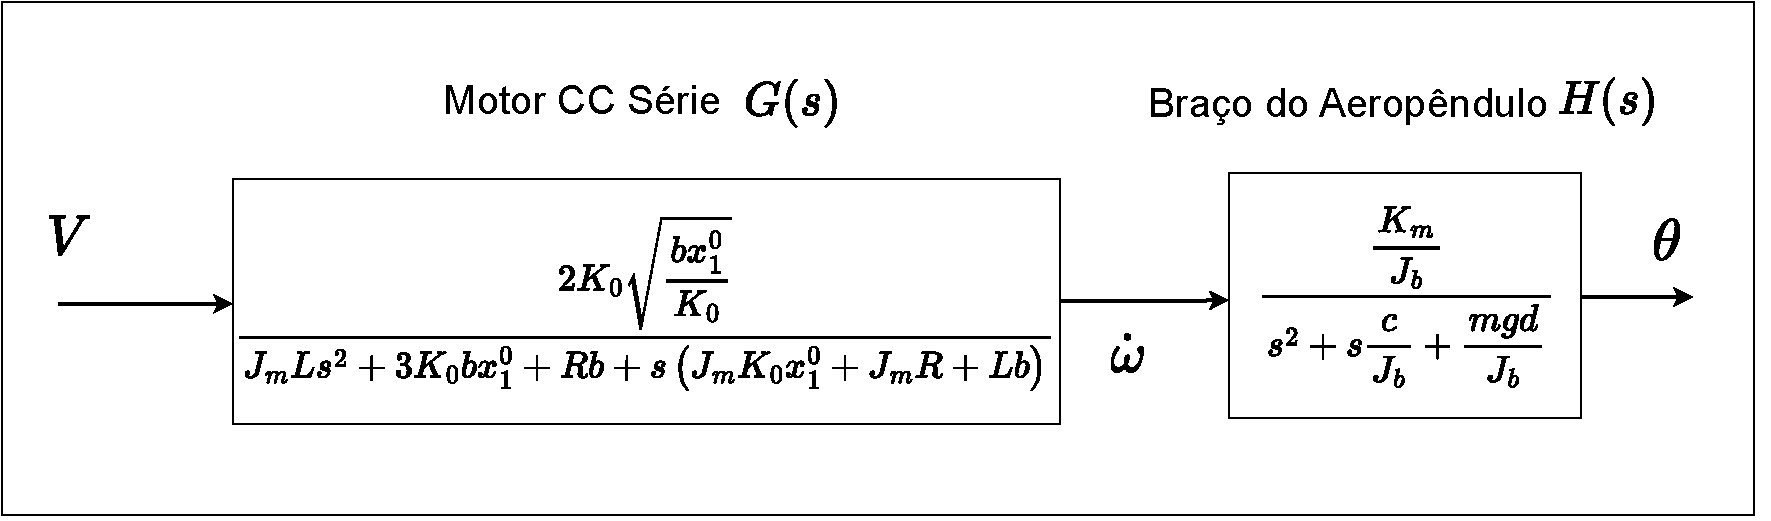
\includegraphics[width=1\textwidth, page=1]{Capitulos/2_aeropendulo/4_figuras/ft_subsistemas.pdf}
	\caption*{Fonte: elaborado pelo autor (2023).}
        \label{fig4:image_05}
\end{figure}



A modelagem usando as leis físicas permite uma interpretação dos parâmetros da planta e ajuda a entender a influência deles na dinâmica do sistema, no entanto, ao utilizar esse método de modelagem surgi uma complexidade em obter os valores numéricos de alguns desses parâmetros, por exemplo, o Momento de Inércia do Eixo do Motor $J_m$ se torna complicado de se obter, assim como o Coeficiente de Amortecimento Viscoso $c$ do pivô do braço do Aeropêndulo entre outros parâmetros, com isso, surgi um método alternativo que permite modela um sistema usando dados de ensaios chamado de Identificação de Sistema, esse método usando os dados de entrada e saída e aproxima um modelo, com isso se obtêm uma função de transferência discreta.

% \section{Modelagem por Identificação de Sistemas}
%\label{model_ident_sis}
%Segundo \cite{aguirre2004intro}, A identificação de sistemas se propõe a obter um modelo matemático que explique, pelo menos em parte e de forma aproximada, a relação de causa e efeito presente nos dados. Isso permite ter uma relação entrada/saída, em que é determinada por meio de uma equação.

CONTINUA ...

%#############################################################################

\newpage
\section{Implementação do Protótipo}
\label{implementacao_prototipo}

\subsection{Protótipo Aeropêndulo}
O projeto para o desenvolvimento do protótipo consiste em uma estrutura mecânica e componentes eletrônicos, a Figura \ref{fig3:image_01} mostra o protótipo finalizado com a parte estrutural e elétrica montada.


\begin{figure}[!h]
	\centering
	\caption{Protótipo do Aeropêndulo.}
	\efbox{\includegraphics[width=0.9\textwidth]{Capitulos/3_hardware_softwares/3_figuras/prot_final.pdf}}
	\caption*{Fonte: elaborado pelo autor (2023).}
	\label{fig3:image_01}
\end{figure}


\subsection{ Parte estrutural do sistema}

 O material escolhido para a estrutura foi o compensado, as chapas de compensado são materiais versáteis e amplamente utilizados na indústria da construção, marcenaria e artesanato. Elas são fabricadas a partir de finas lâminas de madeira, conhecidas como lâminas de folheado, coladas umas sobre as outras com fibras perpendiculares, conferindo maior estabilidade e resistência mecânica ao produto final, Figura \ref{fig3:image_02}.


\begin{figure}[!h]
	\centering
	\caption{Chapas de compensado.}
	\efbox{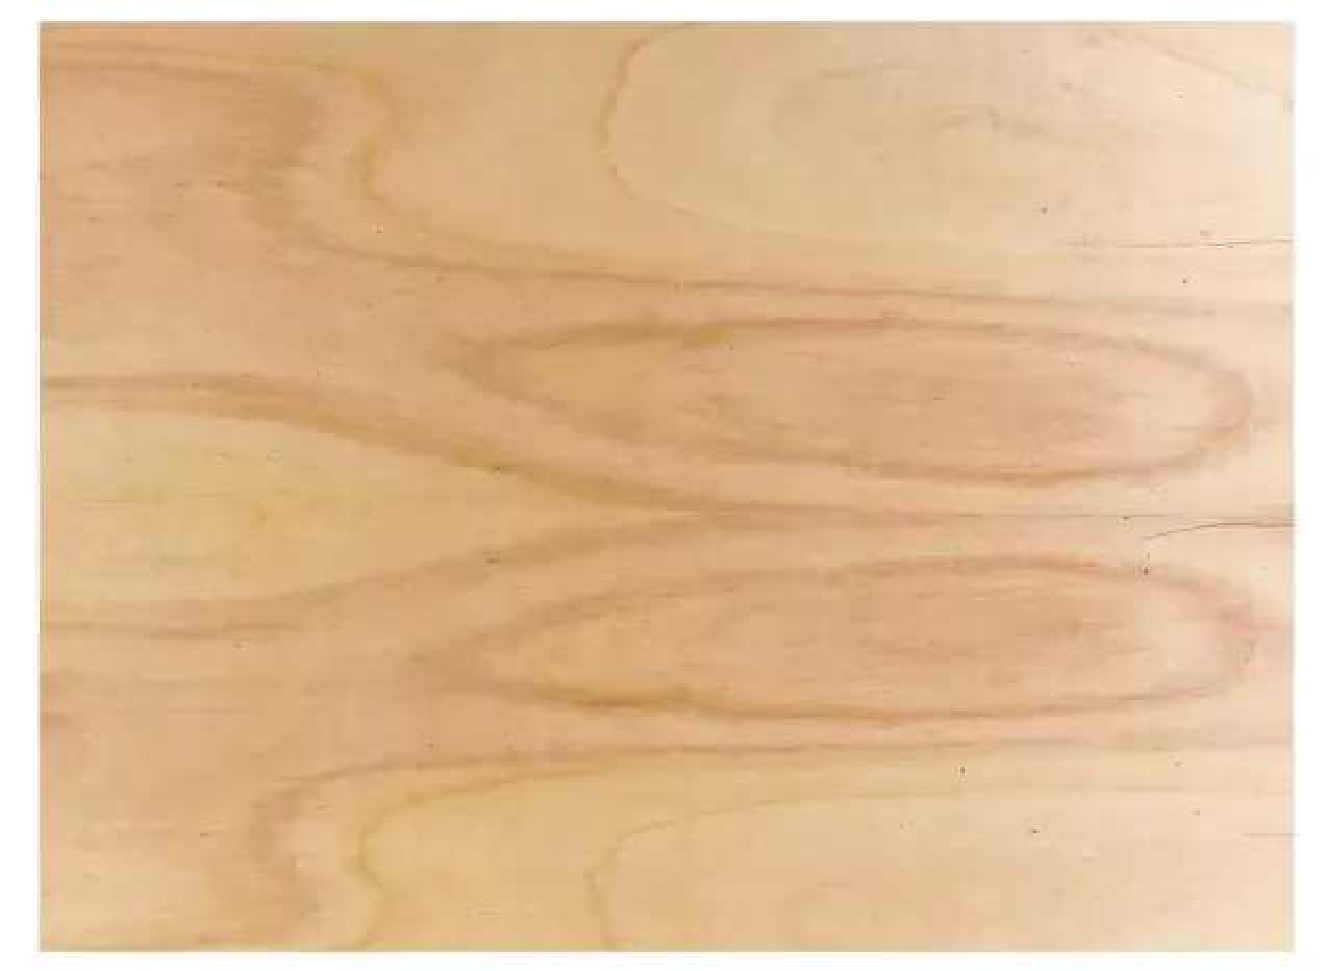
\includegraphics[width=0.6\textwidth]{Capitulos/3_hardware_softwares/3_figuras/compensado.pdf}}
	\caption*{Fonte: elaborado pelo autor (2023).}
	\label{fig3:image_02}
\end{figure}

\newpage
 Já para o braço do Aeropêndulo foi usando Tubo de Fibra de Vidro de Carbono 3x3x2mm, Figura \ref{fig3:image_03}, este material destaca-se por sua leveza e resistência física. No caso do braço do Aeropêndulo, localizado em sua extremidade, há um conjunto motor/hélice encarregado de impulsionar a dinâmica do sistema. Para otimizar o desempenho, é essencial minimizar a massa do braço. Ao fazer isso, as forças de resistência enfrentadas pela força de empuxo serão reduzidas, resultando em uma dinâmica mais ágil e eficiente do sistema.

\begin{figure}[!h]
	\centering
	\caption{Tubo de Fibra de Vidro de Carbono 3x3x2mm.}
	\efbox{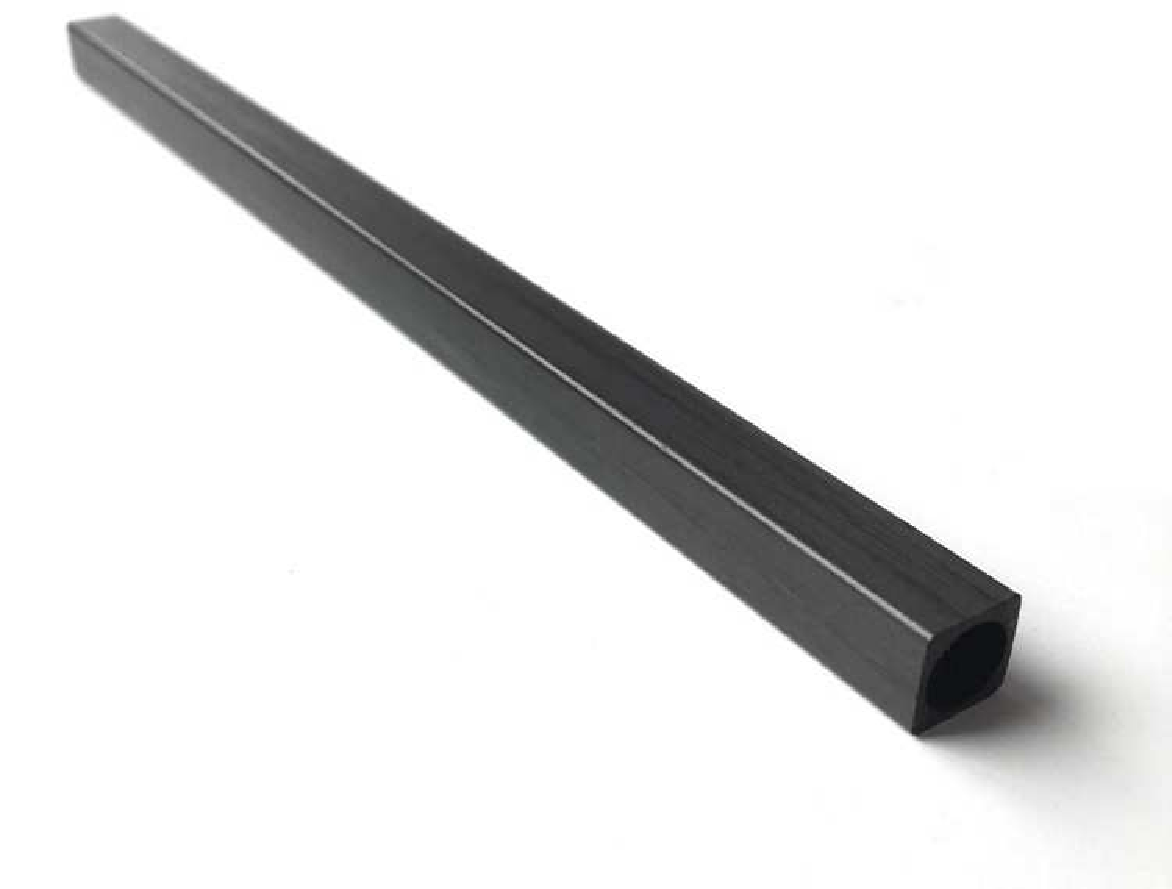
\includegraphics[width=0.5\textwidth]{Capitulos/3_hardware_softwares/3_figuras/carbono2x2mm.pdf}}
	\caption*{Fonte: elaborado pelo autor (2023).}
	\label{fig3:image_03}
\end{figure}


\subsection{Parte Elétrica do sistema}

Foram empregados os seguintes componentes eletrônicos no projeto: um Potenciômetro $50k\Omega$, uma Placa de desenvolvimento Esp32, um Módulo Driver L298n, um Conjunto (suporte/motor/hélice para drones fpv racing quadcopter) e componentes eletrônicos (resistor, capacitor).

\subsubsection{Potenciômetro $50k\Omega$}

O potenciômetro, Figura \ref{fig3:image_04}, desempenha o papel de \textit{encoder} ao obter o ângulo de inclinação do braço do Aeropêndulo. Essa funcionalidade é viabilizada pelo fato de que, conforme o braço se movimenta, a resistência do potenciômetro se altera, resultando em uma variação na tensão registrada em seus terminais. Essa interação permite estabelecer uma correlação entre a mudança na tensão elétrica e o ângulo de inclinação do braço do Aeropêndulo de maneira precisa e controlada.

\begin{figure}[!h]
	\centering
	\caption{Potenciômetro $50k\Omega$.}
	\efbox{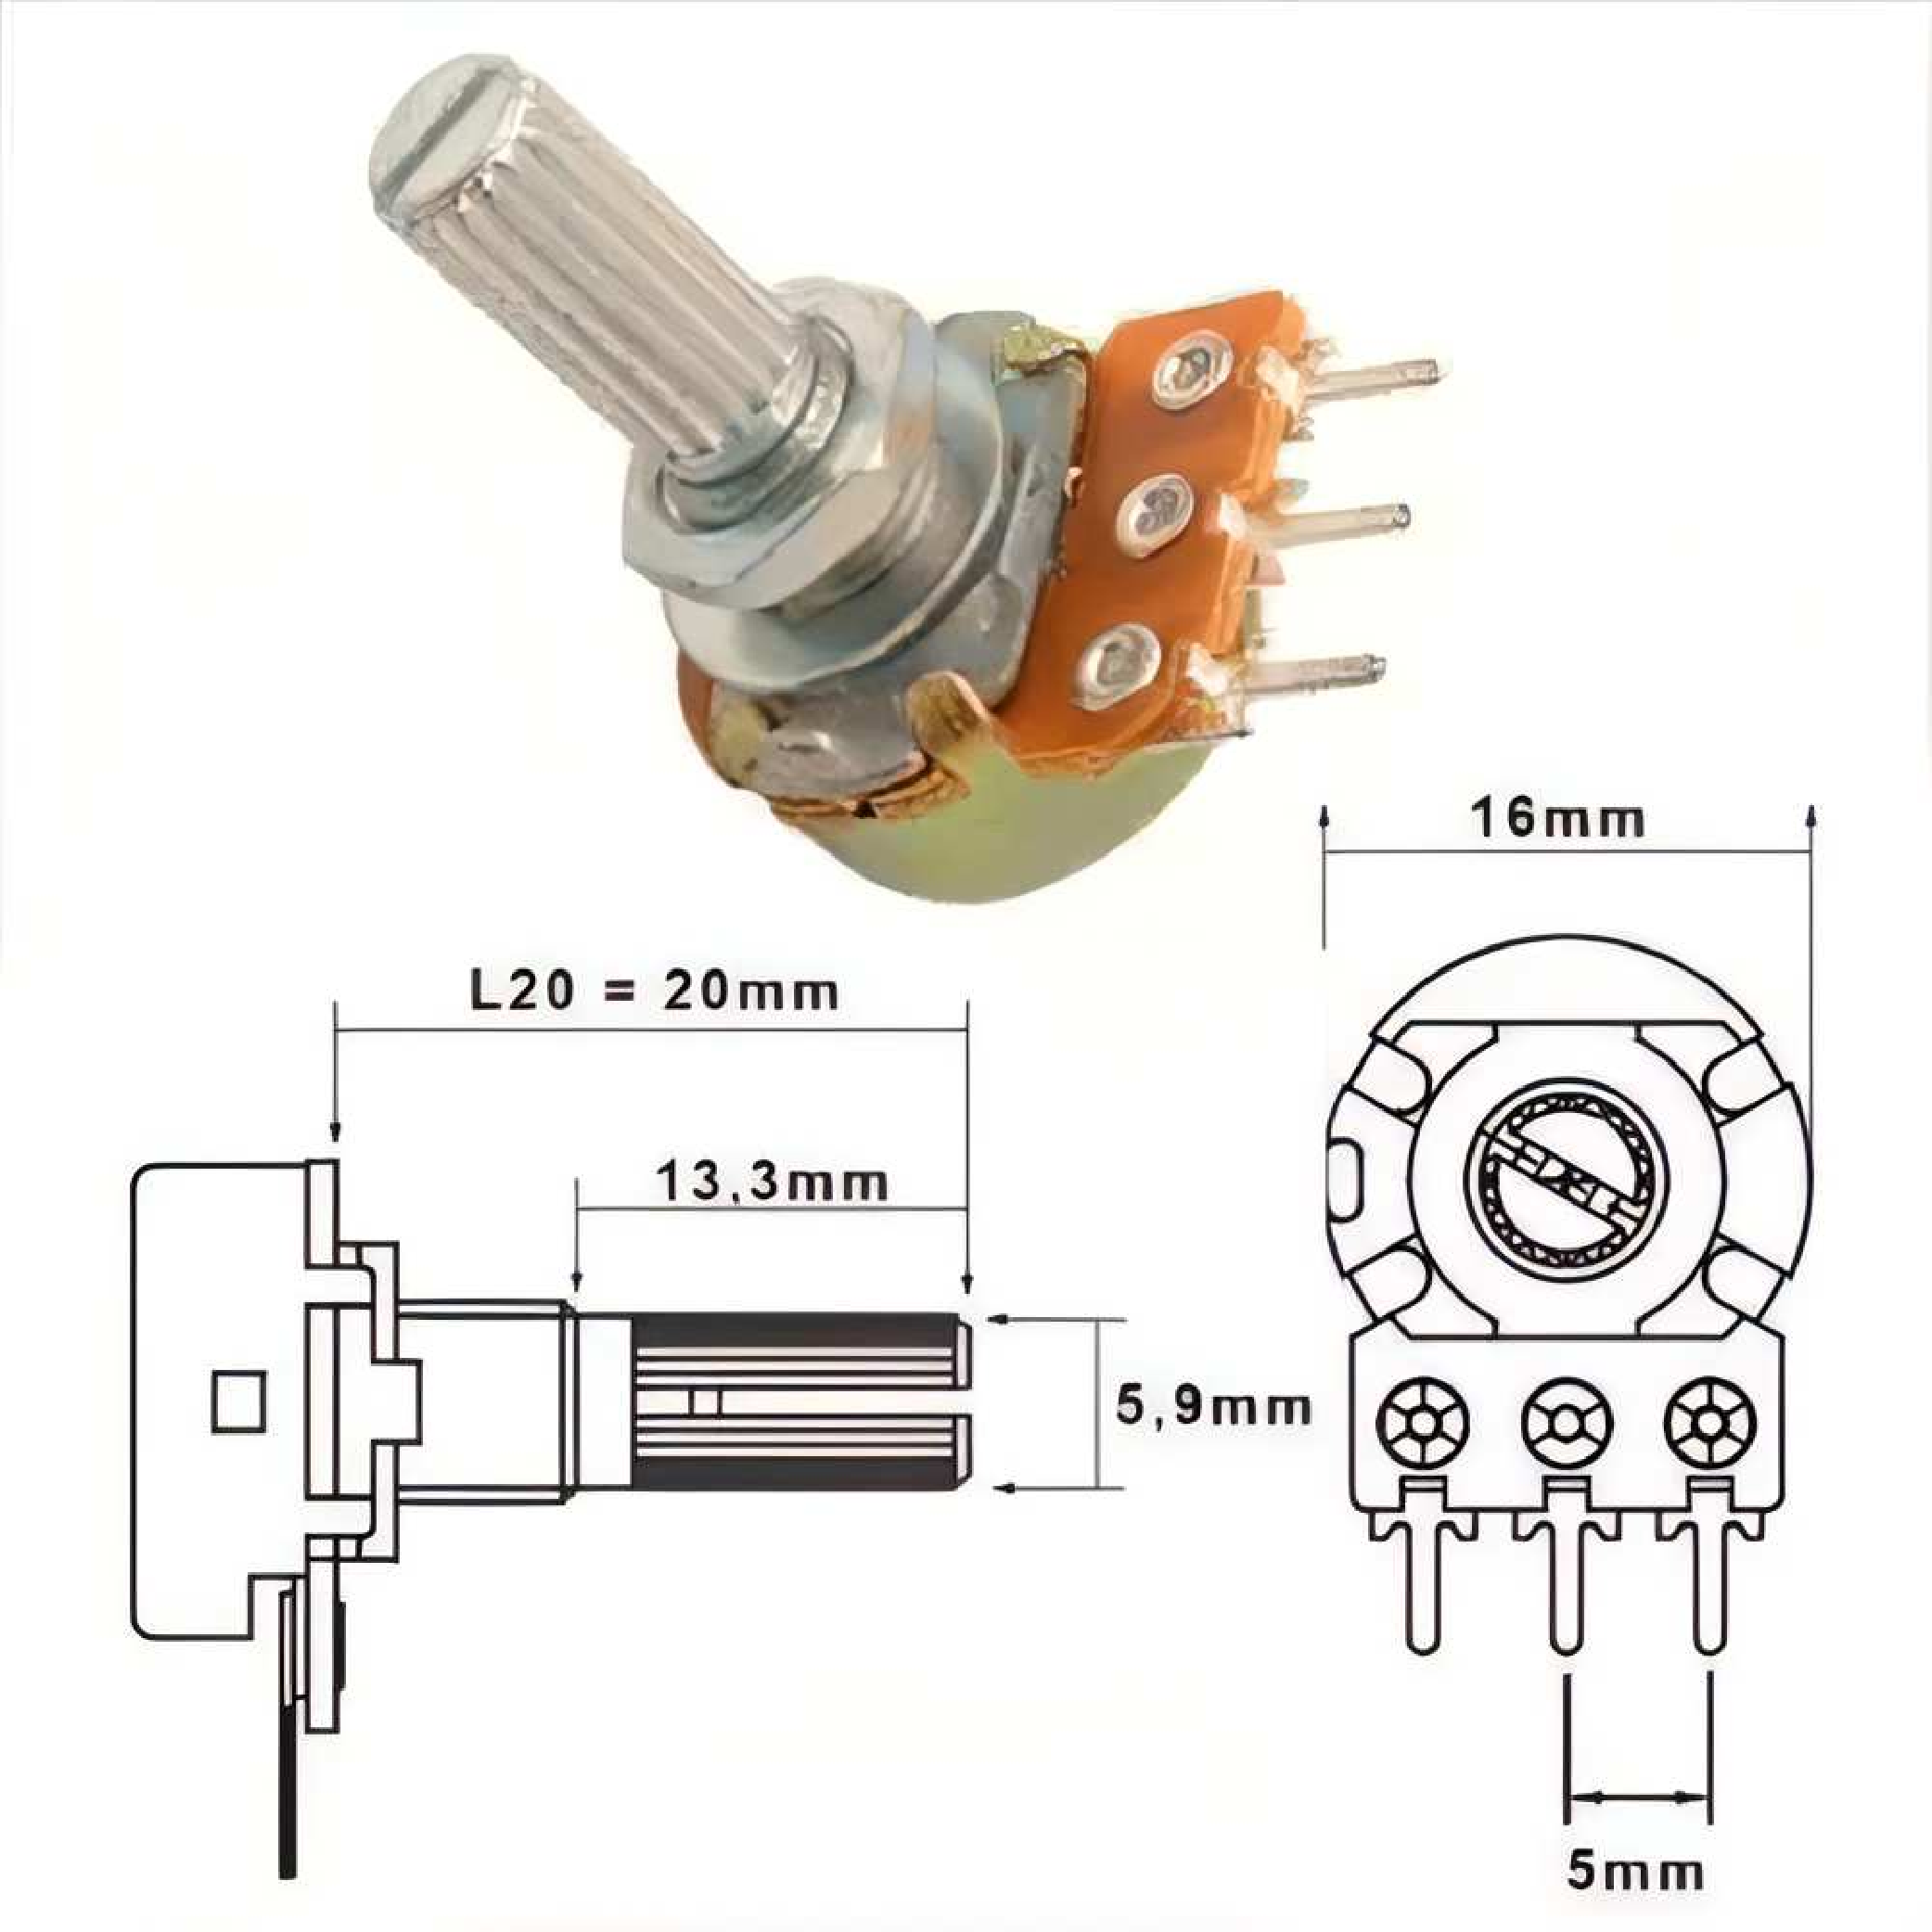
\includegraphics[width=0.5\textwidth]{Capitulos/3_hardware_softwares/3_figuras/pote.pdf}}
	\caption*{Fonte: elaborado pelo autor (2023).}
	\label{fig3:image_04}
\end{figure}




\subsubsection{Placa de desenvolvimento Esp32}

A placa de desenvolvimento ESP32 é uma poderosa e versátil plataforma que integra o popular microcontrolador ESP32 desenvolvido pela empresa  \textit{Espressif}. Projetada para atender às demandas de projetos de Internet das Coisas (IoT) e aplicações de conectividade sem fio, a ESP32 oferece uma vasta gama de recursos e funcionalidades. Equipada com um processador dual-core de 32 bits, Wi-Fi, Bluetooth, interfaces GPIO, I2C, SPI e UART, bem como suporte para memória externa.

A placa desempenhará uma função central no projeto, servindo tanto para a implementação do controlador discreto quanto para a obtenção de dados em tempo real relacionados aos estados do sistema. Esses estados incluem a leitura do sensor de ângulo do braço, a aquisição do sinal de controle e o cálculo do sinal de erro. Adicionalmente, a placa será empregada na geração dos sinais de referência necessários para o funcionamento ideal do sistema, A figura \ref{fig3:image_05} ilustra a placa de desenvolvimento Esp32.

\begin{figure}[!h]
	\centering
	\caption{Placa de desenvolvimento Esp32.}
	\efbox{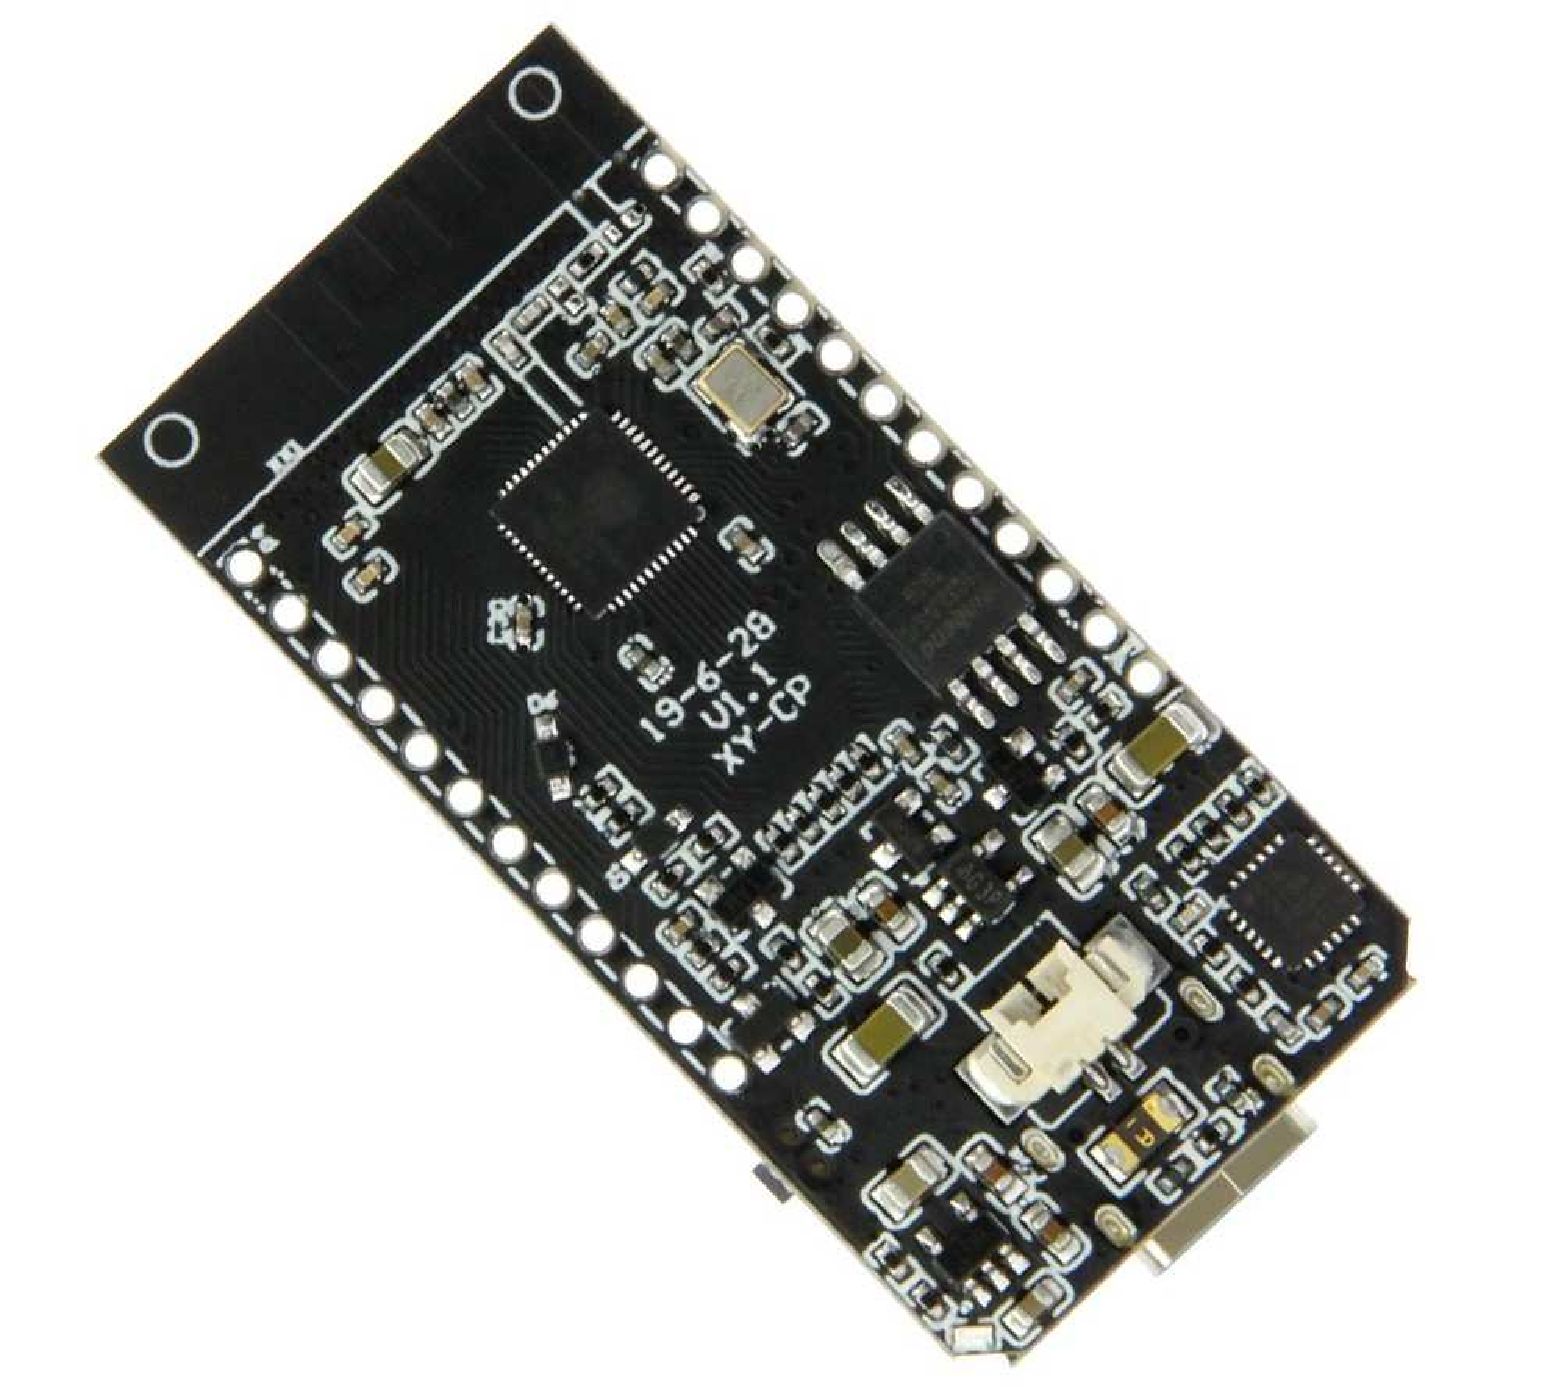
\includegraphics[width=0.5\textwidth]{Capitulos/3_hardware_softwares/3_figuras/f1_esp32.pdf}}
	\caption*{Fonte: elaborado pelo autor (2023).}
	\label{fig3:image_05}
\end{figure}


\subsubsection{Fonte Chaveada 2A, 5V, 25W}

Para a alimentação do motor CC série, foi usado uma fonte de alimentação de 5V/5A, Figura \ref{fig3:image_06}.

\begin{figure}[!h]
	\centering
	\caption{Fonte Chaveada 2A, 5V, 25W.}
	\efbox{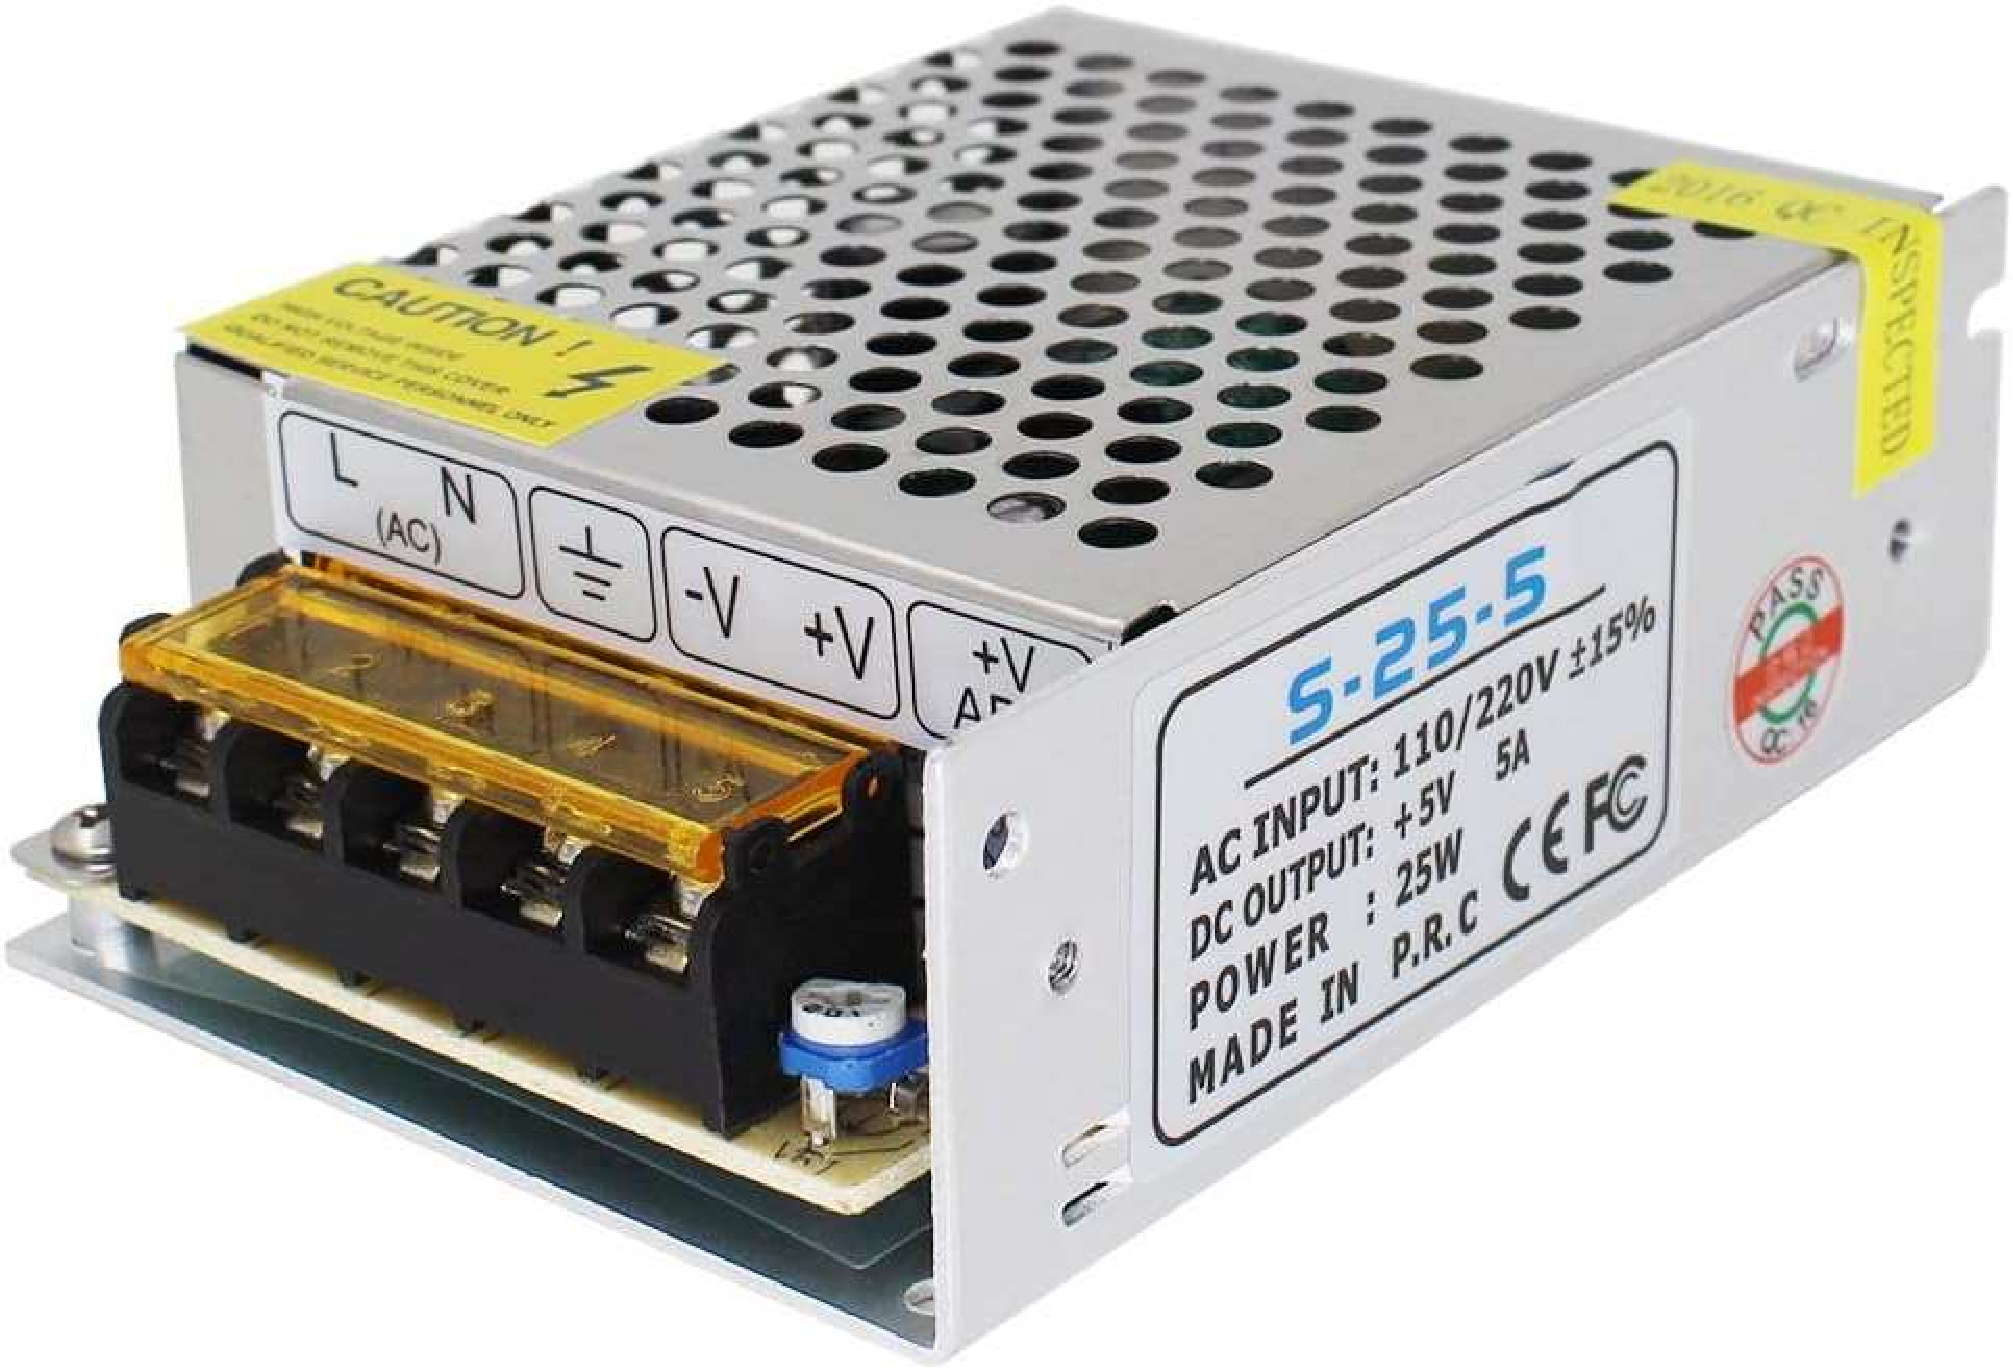
\includegraphics[width=0.45\textwidth]{Capitulos/3_hardware_softwares/3_figuras/f1_fonte.pdf}}
	\caption*{Fonte: elaborado pelo autor (2023).}
	\label{fig3:image_06}
\end{figure}



\subsubsection{Módulo Driver L298n}
\label{driver_l298n}

Para regular a velocidade no eixo do Motor CC série, empregou-se um Módulo Driver L298n, o qual possibilita controlar a injeção de potência entregue ao motor mediante a aplicação de um sinal PWM em sua entrada. Dessa forma, ao ajustar o sinal PWM, é possível obter uma tensão controlada aplicada de maneira precisa aos terminais do motor. A Figura \ref{fig3:image_07} ilustra o componente em questão.

\begin{figure}[!h]
	\centering
	\caption{Módulo Driver L298n.}
	\efbox{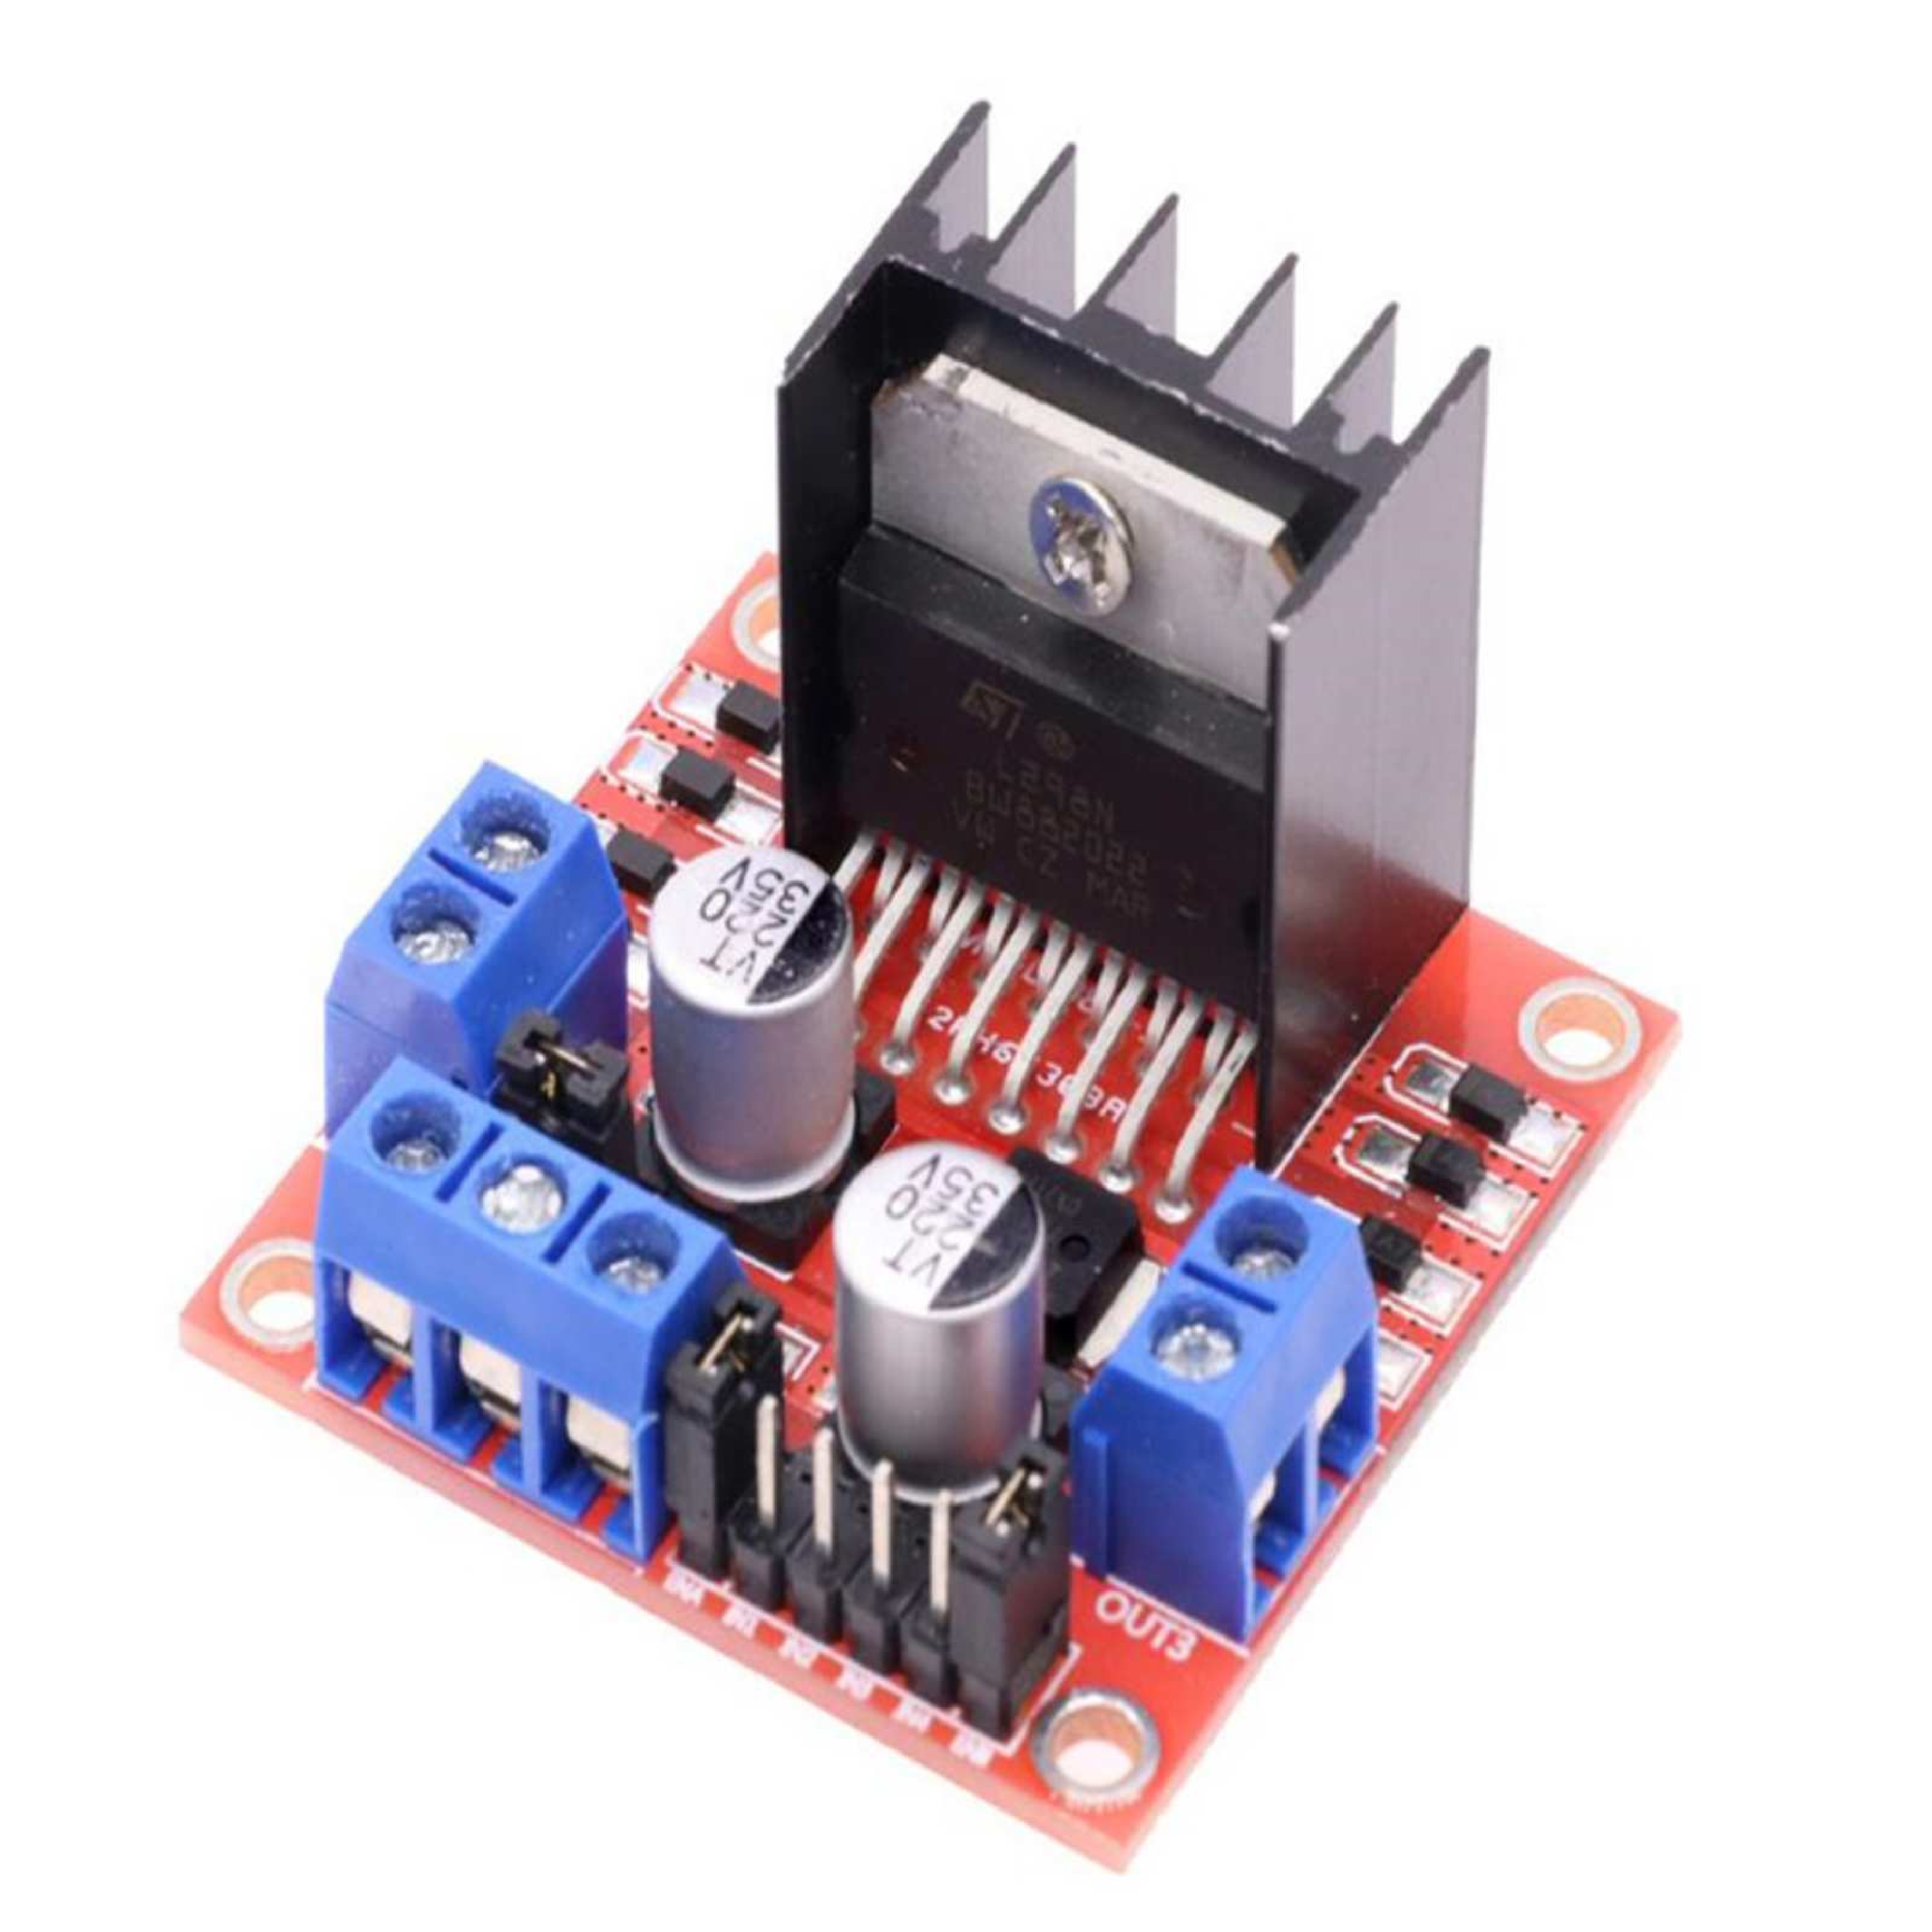
\includegraphics[width=0.45\textwidth]{Capitulos/3_hardware_softwares/3_figuras/f4_ponteH.pdf}}
	\caption*{Fonte: elaborado pelo autor (2023).}
	\label{fig3:image_07}
\end{figure}


\subsubsection{Conjunto (suporte motor cw/ccw hélice) para drones fpv racing quadcopter}


A obtenção da força de empuxo na extremidade do braço do Aeropêndulo foi realizada por meio de um conjunto composto por suporte, motor e hélice projetado originalmente para drones FPV Racing Quadcopter. Esse conjunto demonstrou ser ideal para aplicação no Aeropêndulo devido à sua eficiência e desempenho em ambientes dinâmicos. A Figura \ref{fig3:image_08} fornece uma representação visual esclarecedora desse componente crucial, destacando sua integração perfeita no contexto do experimento.


\begin{figure}[!h]
	\centering
	\caption{Conjunto (suporte motor cw/ccw hélice).}
	\efbox{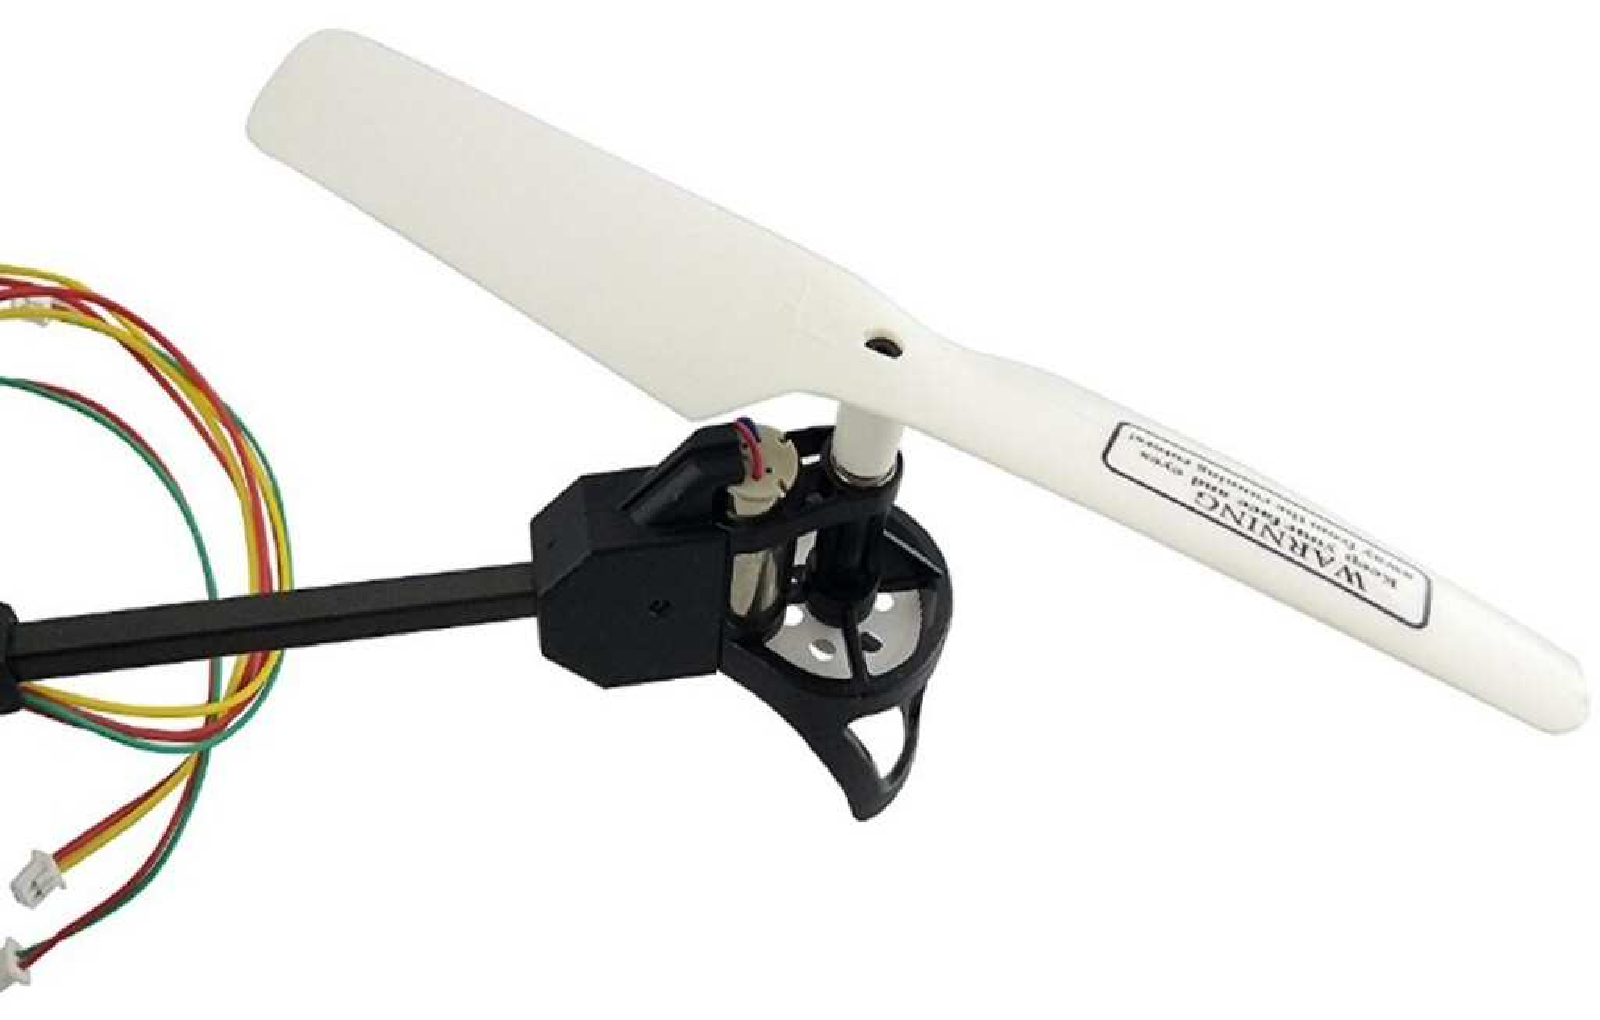
\includegraphics[width=0.5\textwidth]{Capitulos/3_hardware_softwares/3_figuras/f1_braco_aerop.pdf}}
	\caption*{Fonte: elaborado pelo autor (2023).}
	\label{fig3:image_08}
\end{figure}

\newpage
\subsubsection{Componentes eletrônicos (resistivos e capacitivos)}

Por fim, para que o sinal do sensor (Potenciômetro) seja de boa qualidade, foi usado um filtro RC série, dessa forma, empregou-se um capacitor de um resistor na implementar do filtro. A Figura \ref{fig3:image_09} corresponde aos componentes resistivos e a Figura \ref{fig3:image_10} aos componentes capacitivos.


\begin{figure}[!h]
         \centering
         \caption{Resistores.}
         \efbox{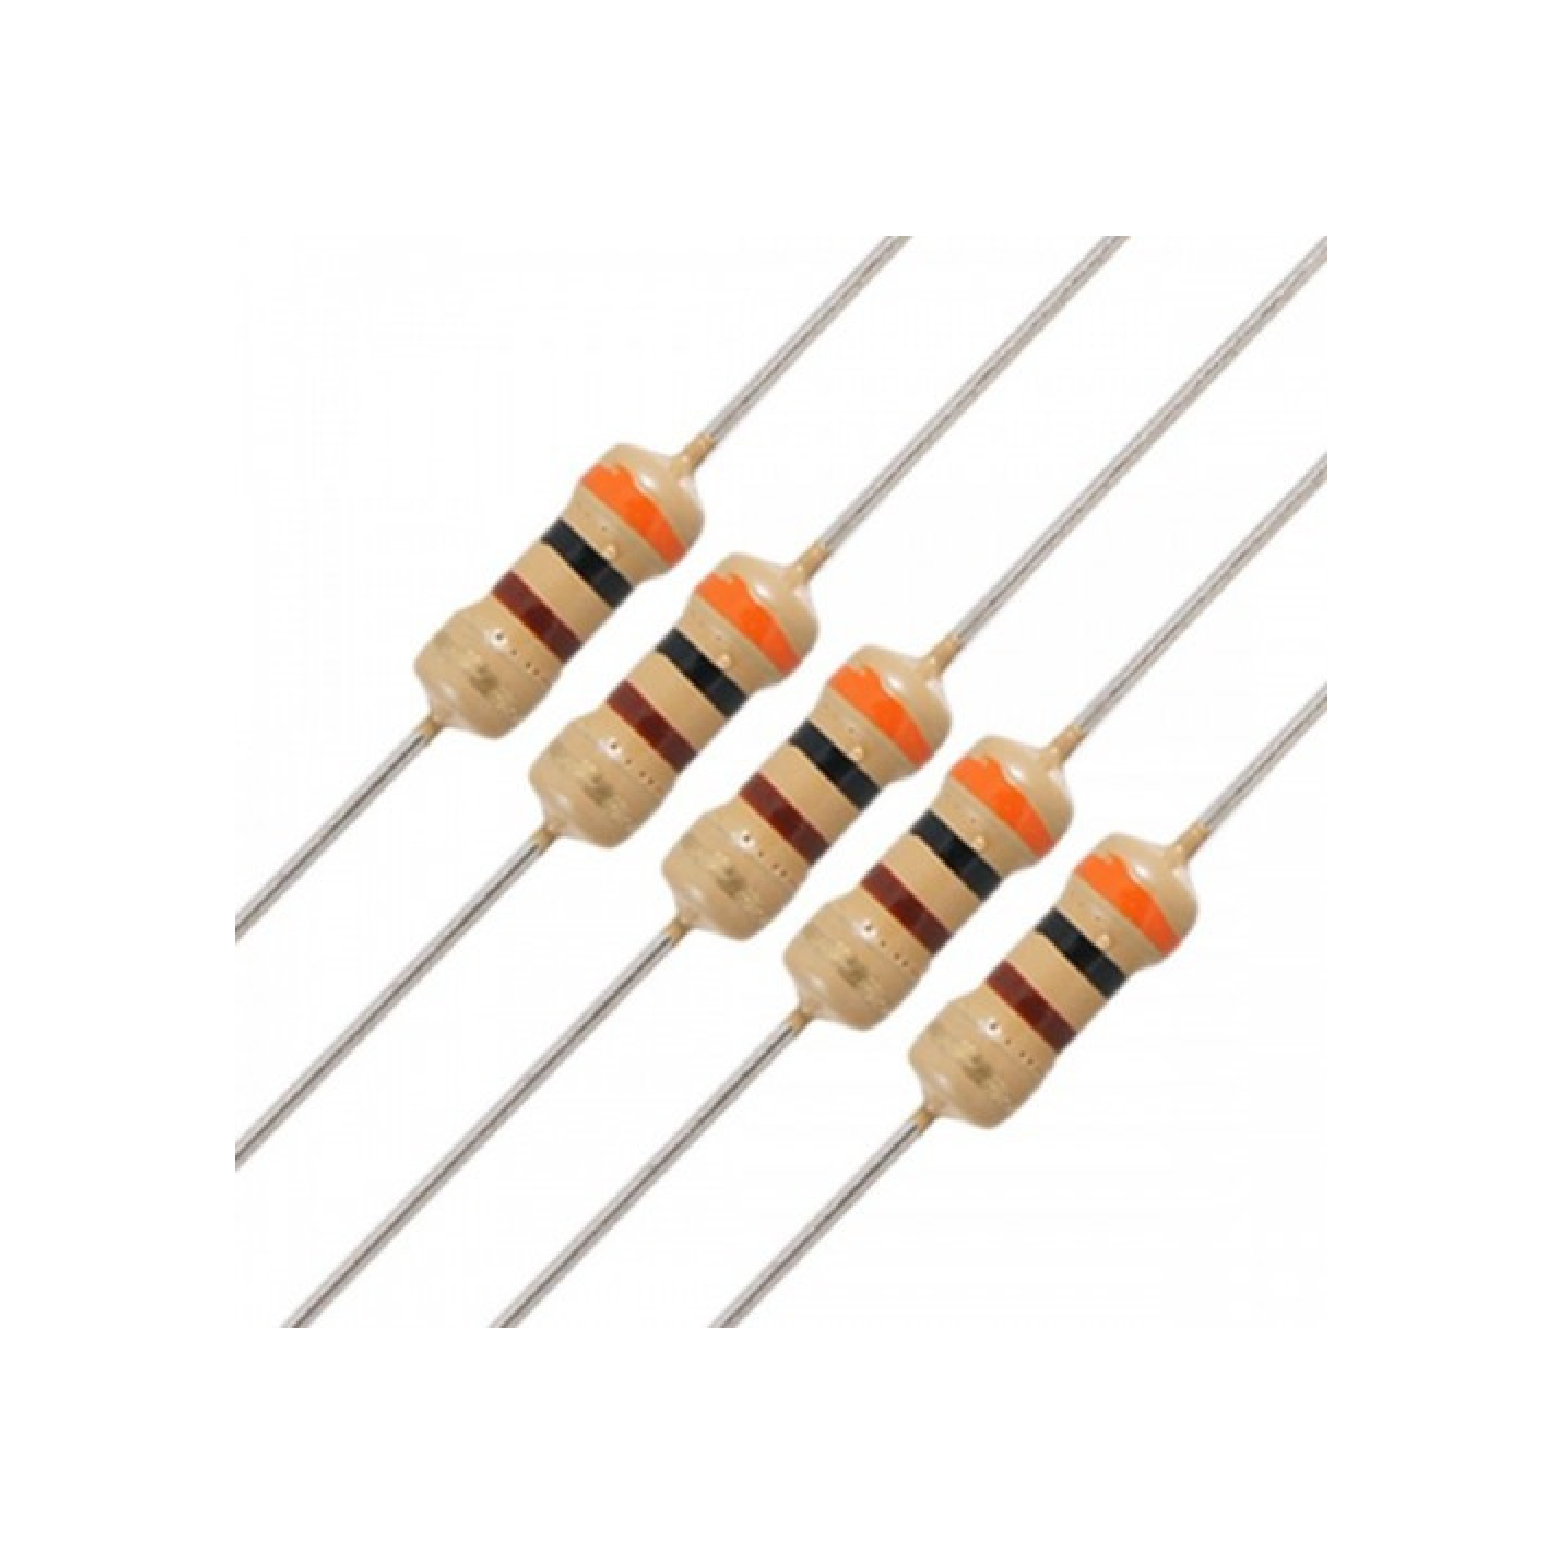
\includegraphics[width=0.5\textwidth, page=1]{Capitulos/3_hardware_softwares/3_figuras/res_cap.pdf}}
         \caption*{Fonte: elaborado pelo autor (2023).}
         \label{fig3:image_09}
\end{figure}

\begin{figure}[!h]
         \centering
         \caption{Capacitores.}
         \efbox{\includegraphics[width=0.5\textwidth, page=2]{Capitulos/3_hardware_softwares/3_figuras/res_cap.pdf}}
         \caption*{Fonte: elaborado pelo autor (2023).}
         \label{fig3:image_10}
\end{figure}


\subsection{Montagem do Protótipo}

\subsubsection{Parte Física}

O protótipo foi concebido visando a desmontagem da estrutura, permitindo um transporte mais conveniente. A construção física compreende três componentes com pontos de conexão estratégicos. Ademais, o braço do Aeropêndulo pode ser facilmente desacoplado no ponto de pivô, onde se conecta ao eixo do potenciômetro.

Para montar a estrutura, basta acoplar suas partes. Com isso, a componente estrutural estará pronta para uso. O resultado final do sistema ficou notavelmente estável, com a estrutura demonstrando rigidez suficiente para evitar vibrações indesejadas no braço do Aeropêndulo durante o acionamento.

\subsubsection{Parte Elétrica}


A Figura \ref{fig3:image_11} ilustra a dinâmica do fluxo de interligação do sistema elétrico do Aeropêndulo. Notavelmente, o microcontrolador desempenha um papel central ao gerar o sinal de controle PWM, realiza a leitura do sinal filtrado proveniente do sensor (Potenciômetro) e estabelecer comunicação com o computador através da interface serial. Adicionalmente, o driver é alimentado por uma fonte de tensão contínua de 5V, o qual amplifica e aplica o sinal de controle ao motor CC Série. Esta ação, por sua vez, resulta em uma variação angular no braço do Aeropêndulo por conta do empuxo gerado pelas hélices, impactando diretamente o estado do sensor (Potenciômetro) e sua saída correspondente.

\begin{figure}[!h]
	\centering
	\caption{Diagrama de comunicação do Aeropêndulo.}
	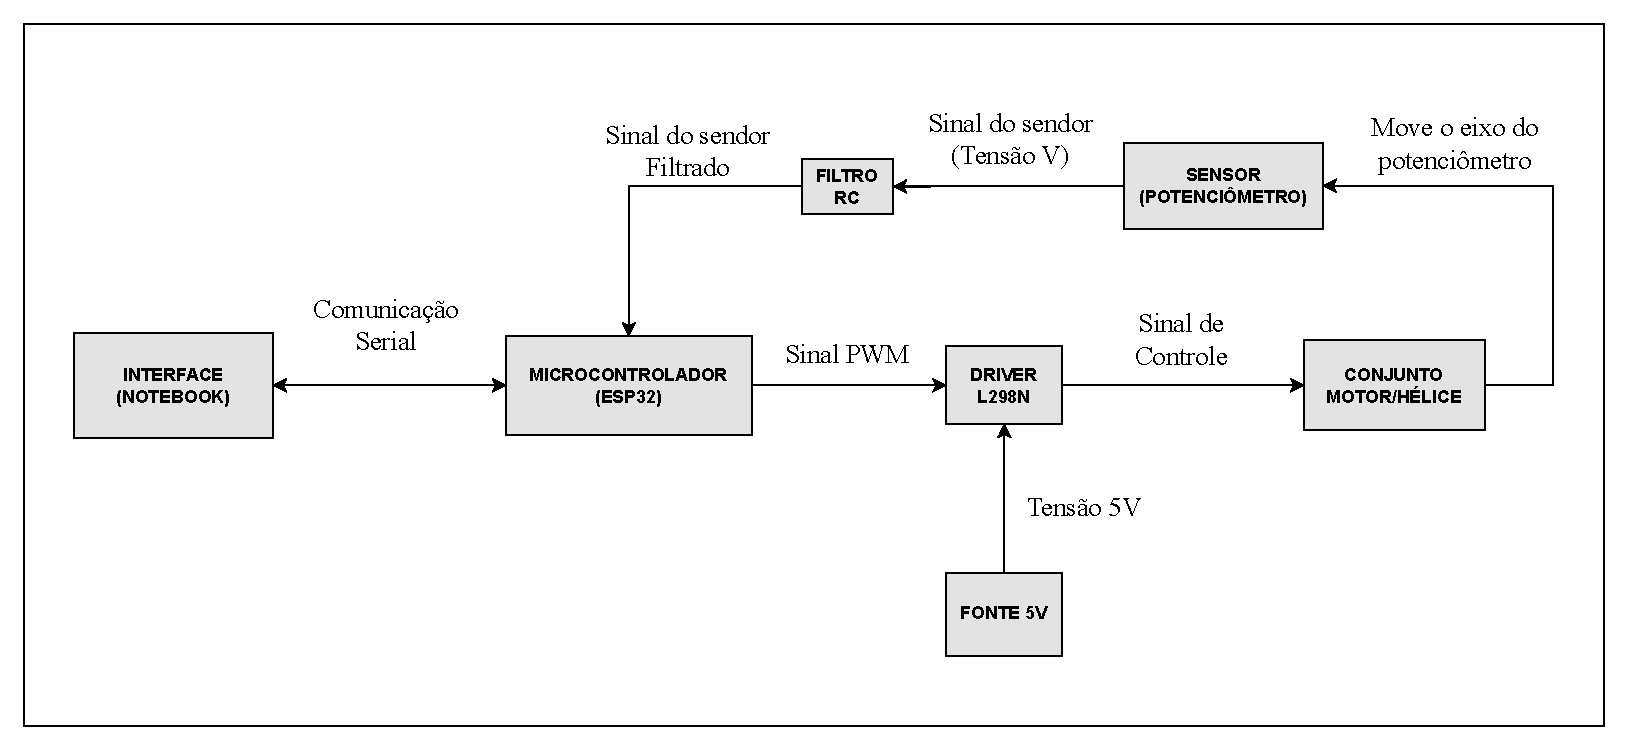
\includegraphics[width=0.9\textwidth, page=1]{Capitulos/3_hardware_softwares/3_figuras/diag_aerop.pdf}
	\caption*{Fonte: elaborado pelo autor (2023).}
	\label{fig3:image_11}
\end{figure}



O esquema de ligação dos componentes do sistema elétrico é exemplificado na Figura \ref{fig3:image_12}.

\begin{figure}[!h]
	\centering
    	\caption{Esquema de conexões elétricas do Aeropêndulo.}
	\efbox{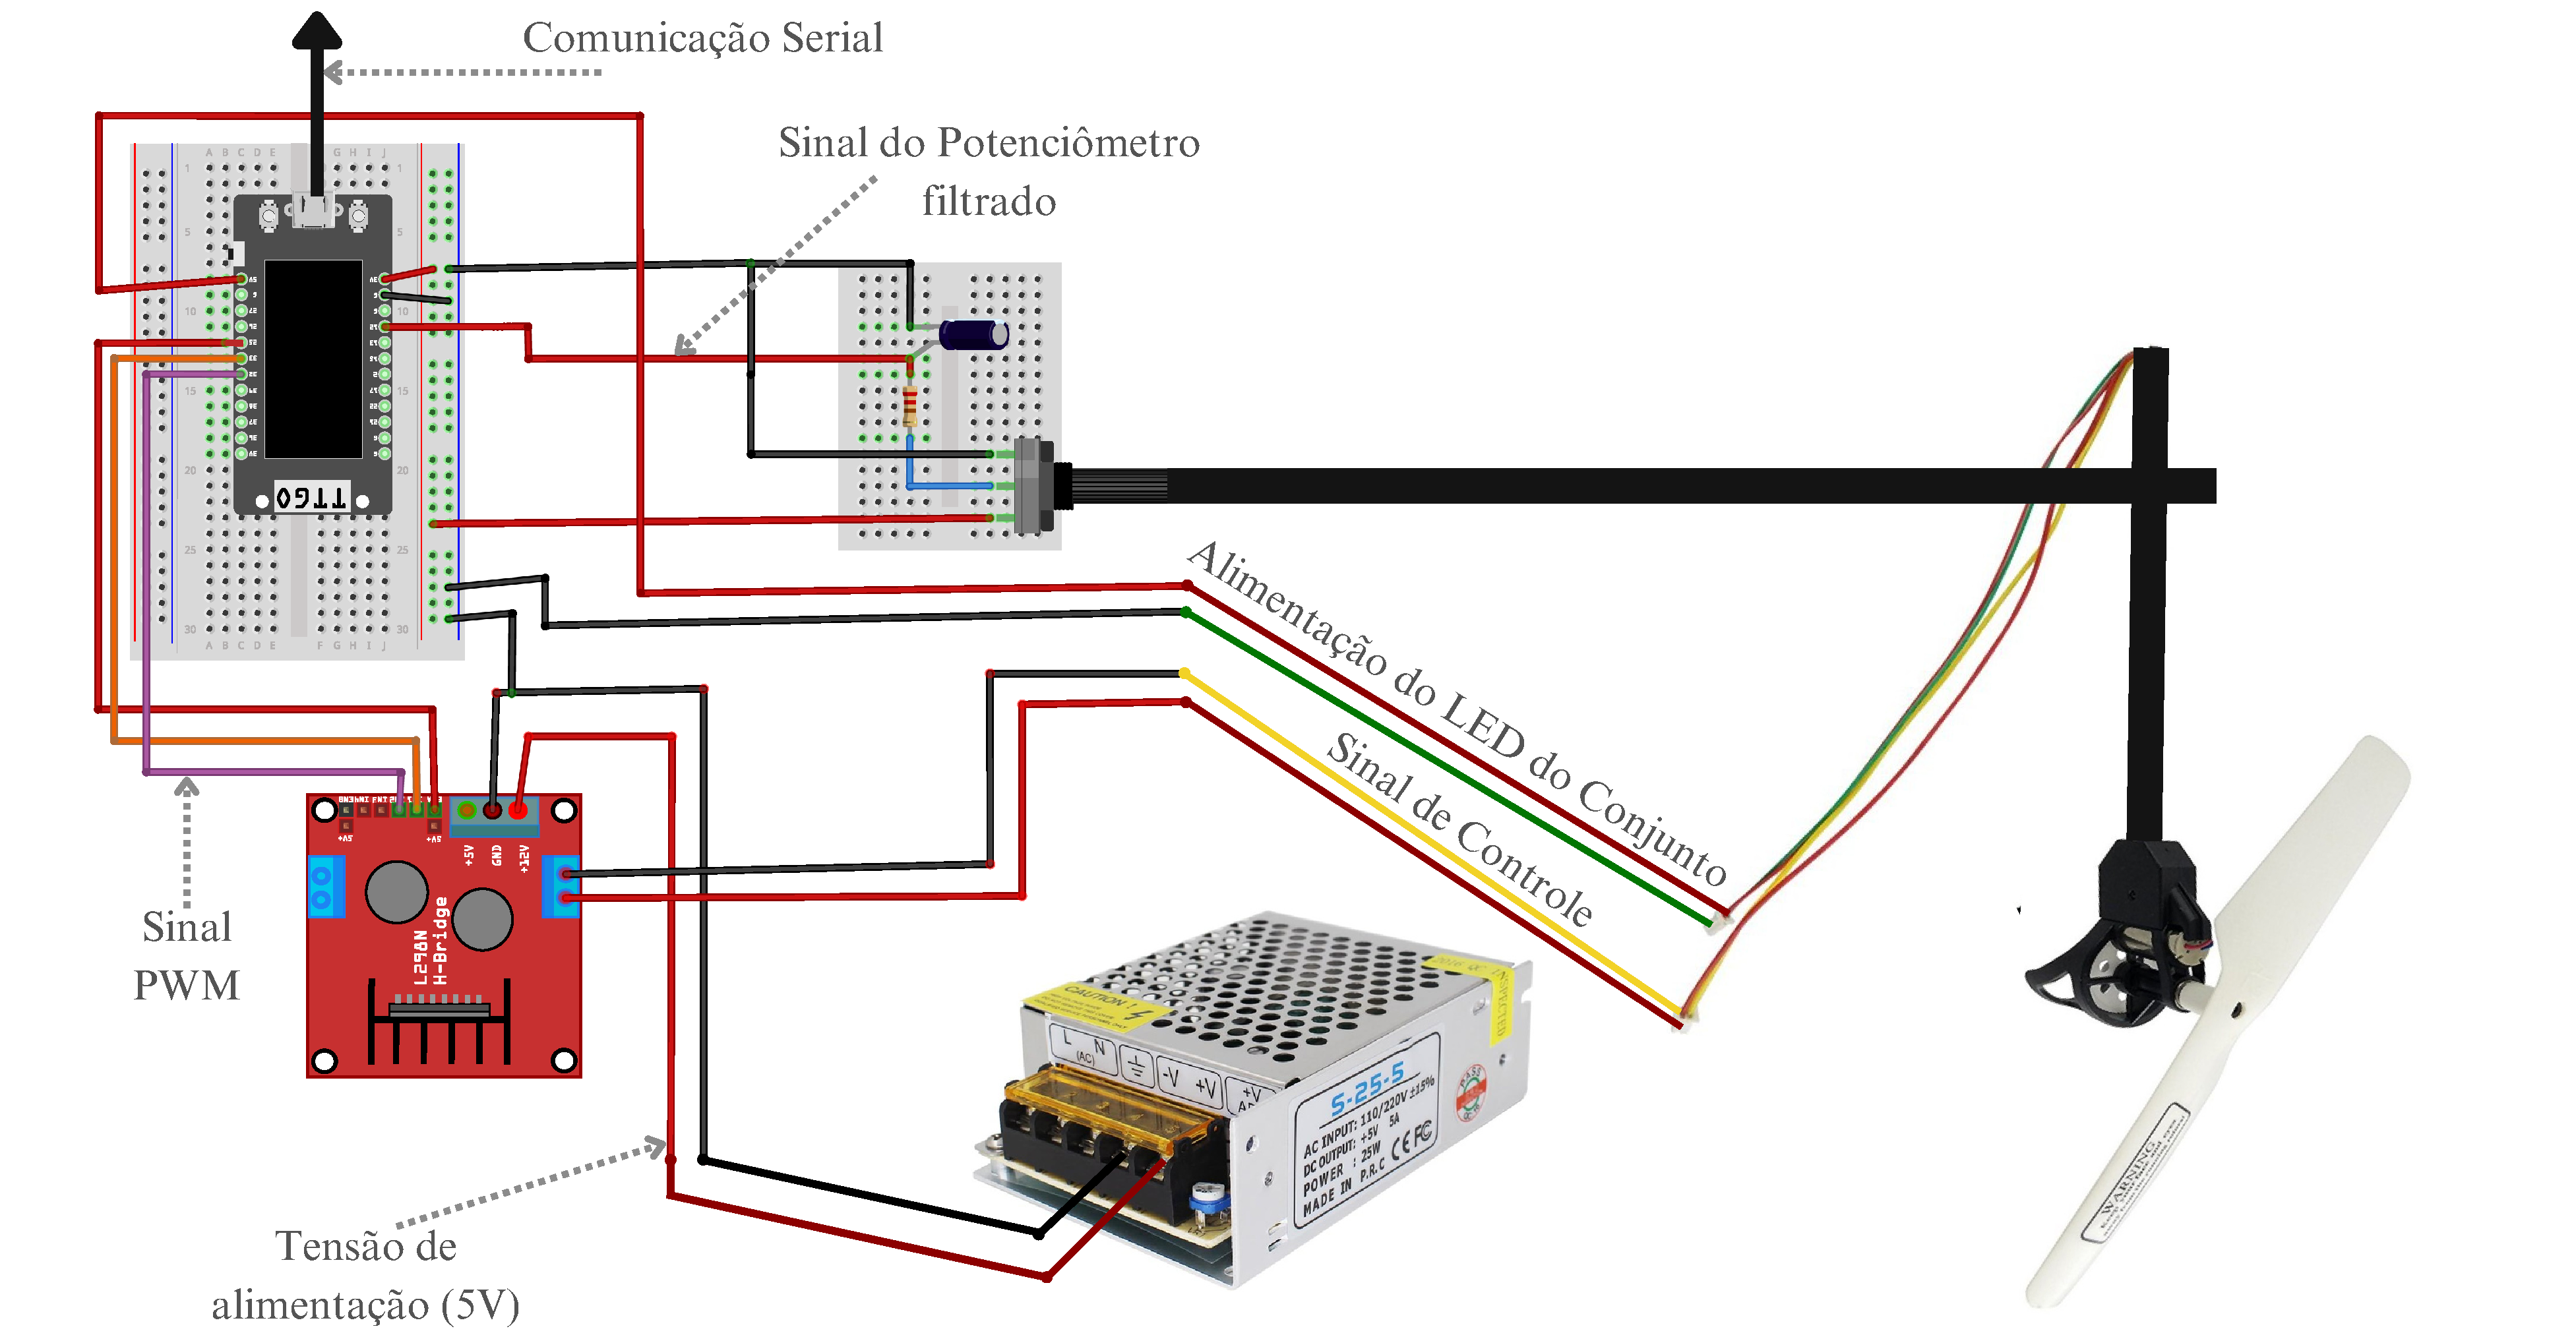
\includegraphics[width=1\textwidth, page=1]{Capitulos/3_hardware_softwares/3_figuras/esquema_eletrico_aerop.pdf}}
	\caption*{Fonte: elaborado pelo autor (2023).}
	\label{fig3:image_12}
\end{figure}

\vspace{2cm}


\section{Desenvolvimento dos Softwares}
\label{dev_softwares}
Para permitir a interação com o protótipo um conjunto de software foi desenvolvido, permitindo aos usuários aplicar diferentes conceitos de sistema de controle e obter uma visualização em tempo real dos estados do sistema através desses softwares, sendo eles, o firmware do microcontrolador, simulador 3D que usa o conceito de Gêmeo Digital, uma interface gráfica com um conjunto de funcionalidades capaz de manipular o sinal de referência e plotar os gráficos dos estados do sistema.

\subsection{Linguagens Python, C e C++}
Para o desenvolvimento dos softwares destinados à visualização de dados e ao simulador, a linguagem de programação escolhida foi o Python. Essa seleção se deu devido à natureza versátil da linguagem, que permite um desenvolvimento ágil de softwares para uma ampla gama de finalidades. Em paralelo, para a programação do microcontrolador, optou-se pelo uso das linguagens C/C++. Essa escolha se fundamenta na ampla adoção dessas linguagens na programação de sistemas embarcados, garantindo um ambiente propício para a eficaz implementação no microcontrolador.

A linguagem Python é amplamente reconhecida como uma linguagem de programação de alta qualidade, interpretada e de propósito geral. Ela desfruta de uma imensa popularidade em todo o mundo e é empregada em diversas aplicações, abrangendo campos como computação científica, ciência de dados, engenharia de software e inteligência artificial. Python se destaca por ser uma linguagem de programação de fácil aprendizado e utilização, mesmo para indivíduos com pouca experiência em codificação. Sua sintaxe clara e concisa contribui para a legibilidade e manutenibilidade do código.

Por essas razões, Python emerge como a escolha ideal para conduzir trabalhos de pesquisa e desenvolvimento. É uma ferramenta incrivelmente versátil e poderosa, capaz de lidar com uma extensa variedade de tarefas, desde a análise de dados até a criação de aplicações complexas.


Já C e C++ são linguagens de programação que se concentram na eficiência e na portabilidade. Elas são amplamente utilizadas no desenvolvimento de sistemas operacionais, drivers de dispositivos, compiladores e outros softwares críticos. C foi criada em 1972 por Dennis Ritchie para o desenvolvimento do sistema operacional Unix. C++ foi criada em 1983 por Bjarne Stroustrup como uma extensão de C para adicionar suporte à programação orientada a objetos.

C e C++ são linguagens de programação poderosas e flexíveis, mas também podem ser complexas e difíceis de aprender. Elas são recomendadas para desenvolvedores que precisam de um alto nível de controle sobre o desempenho e a portabilidade de seu código.


\subsection{ Gêmeo Digital}
Nesta seção, será elaborado o Gêmeo Digital do Aeropêndulo. O Gêmeo Digital representa um sistema gráfico computacional que reproduz em tempo real a dinâmica do protótipo. Isso permite a virtualização do Aeropêndulo, possibilitando a observação da mesma dinâmica do sistema físico, agora em um ambiente gráfico computacional 3D. Essa virtualização é viabilizada pela obtenção do estado atual do braço do Aeropêndulo por meio de comunicação serial.

Para o desenvolvimento do Gêmeo Digital, utilizou-se a biblioteca VPython, essa biblioteca possui um conjunto de funções que permite criar objetos 3D capazes de realizar movimentos rotacionais de translacionais, além disso, é possível plotar gráficos em tempo real. A figura \ref{fig3:image_13_1} ilustra a interface do simulador já finalizado, pode-se observar que a interface é composta de duas partes principais, uma que implementa o ambiente 3D com o Aeropêndulo e a outra gera os gráficos do sinal de referência e de saída.

Com a finalidade de atualizar os estados dos gráficos e a posição angular do gêmeo digital em tempo real a aplicação se comunica com a interface gráfica, subseção \ref{interface_graica}, com isso é possível realizar a atualização dos estados do gráfico assim como do gêmeo digital tendo como entrada os sinais dos estados do protótipo.

\begin{figure}[!h]
	\centering
	\caption{Gêmeo Digital - Simulador com VPython.}
	\efbox{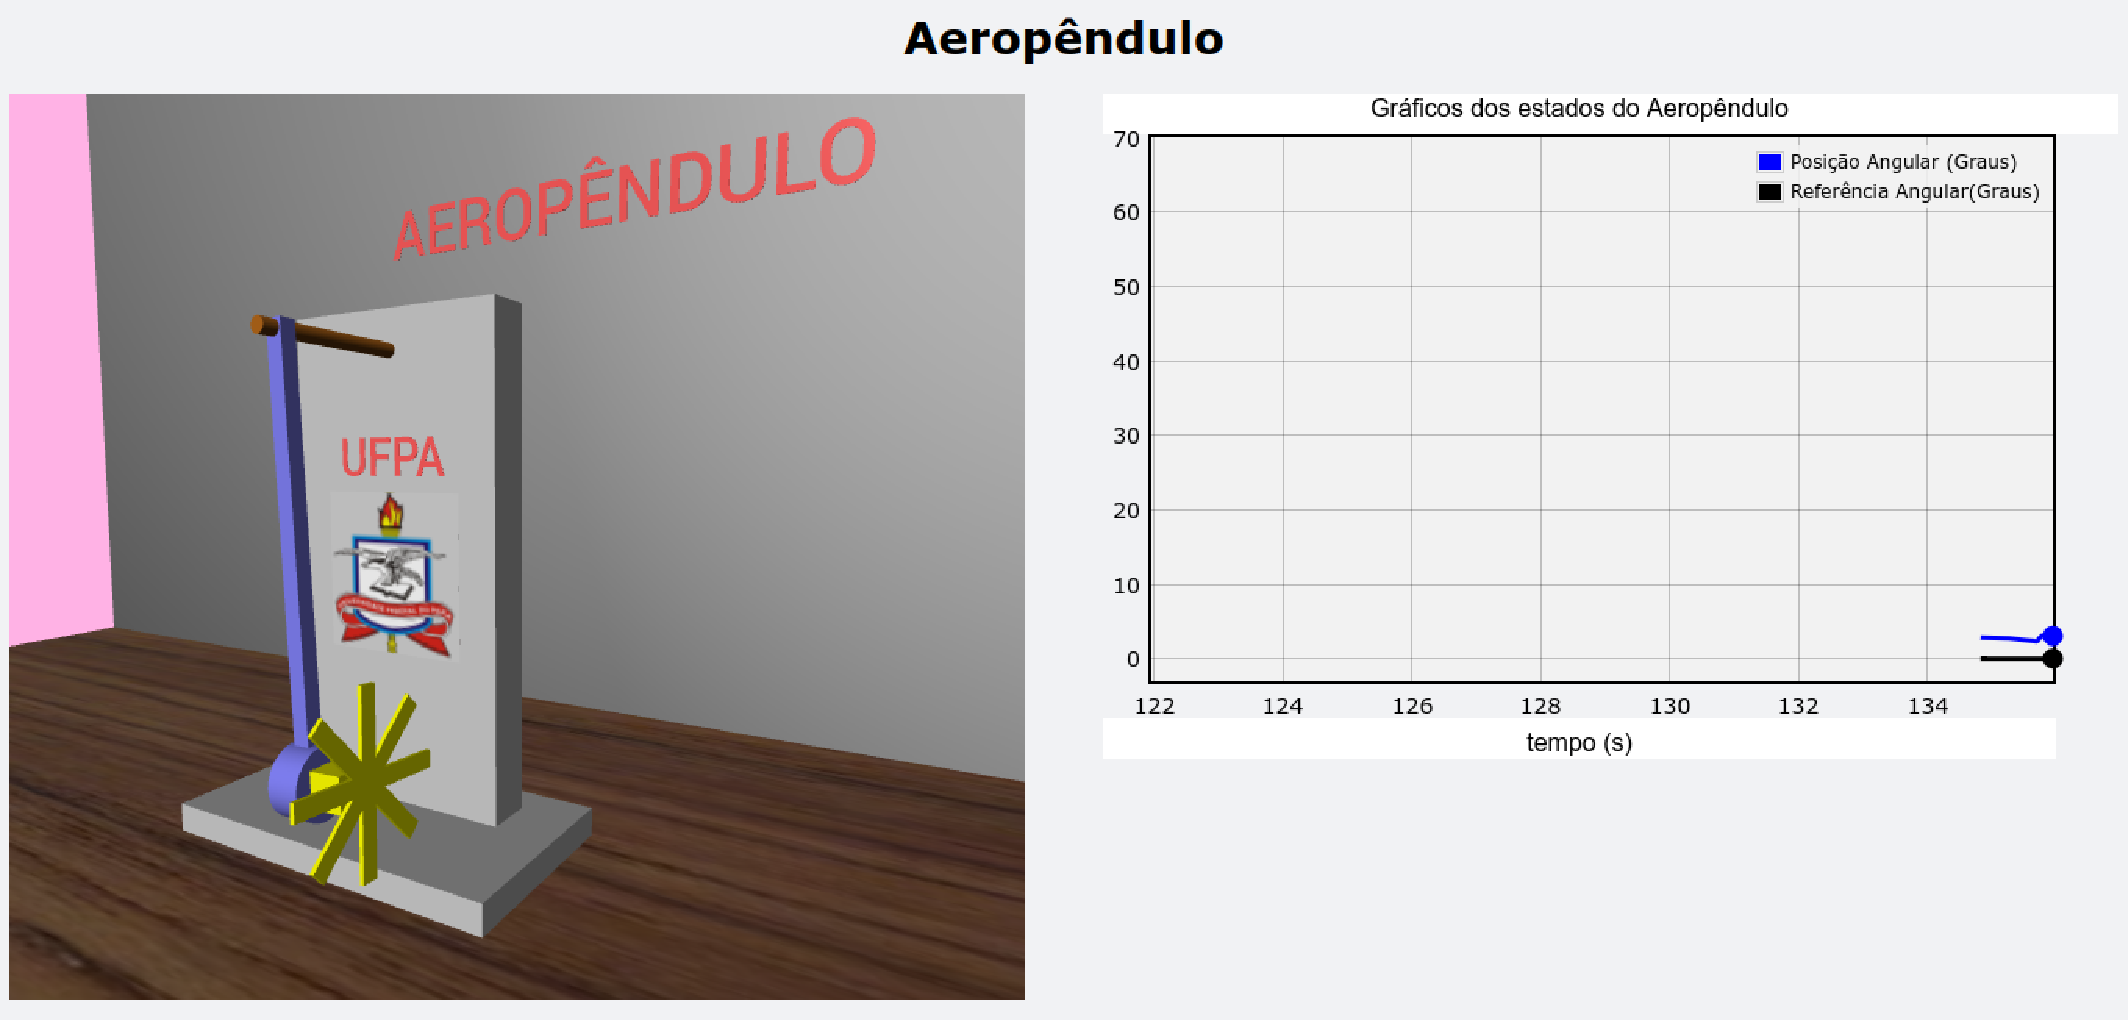
\includegraphics[width=1\textwidth]{Capitulos/3_hardware_softwares/3_figuras/simulador.pdf}}
        \vspace{0.001cm}
	\caption*{Fonte: elaborado pelo autor (2023).}
	\label{fig3:image_13_1}
\end{figure}

% O gêmeo digital do aeropêndulo foi derivado de um projeto que o Autor desse TCC participou, intitulado \textbf{Laboratório Virtual para Sistemas Dinâmicos e Controle na Faculdade de Engenharia Elétrica da UFPA-Tucuruí}, a partir desse projeto foi ...

\newpage
\subsubsection{Biblioteca VPython}

Conforme o site oficial \cite{vpython}, O VPython, por ser desenvolvido com a linguagem Python, é uma ferramenta versátil para a criação de animações 3D navegáveis. Ele é fácil de aprender e usar, mesmo para pessoas com pouca experiência em programação. No entanto, ele também oferece uma ampla gama de recursos para programadores e pesquisadores experientes.

Ao criar uma simulação com VPython e executá-la, o simulador será renderizado no navegador de internet padrão do sistema operacional.


\subsubsection{Arquitetura do Gêmeo Digital}

Para implementar o simulador a arquitetura do sistema consiste de um módulo para gerar os gráficos de linha e outro para desenhar o simulador 3D, existe um módulo que integra e atualiza os estados dos gráficos de linha e do simulador 3D, a figura \ref{fig3:image_13} mostra como a estrutura do simulador foi pensada, o último bloco é a interface gráfica, subseção \ref{interface_graica}, responsável por obter os estados do sistema real, com isso, é possível usar a velocidade angular real do protótipo como entrada para o gêmeo digital, isso faz com que a dinâmica do protótipo seja reproduzida no gêmeo digital, além disse, é possível obter os sinais de referência e de saída e atualizar os gráfios que compõem a interface do simulador.

\begin{figure}[!h]
	\centering
	\caption{Diagrama da arquitetura do Gêmeo Digital.}
	\efbox{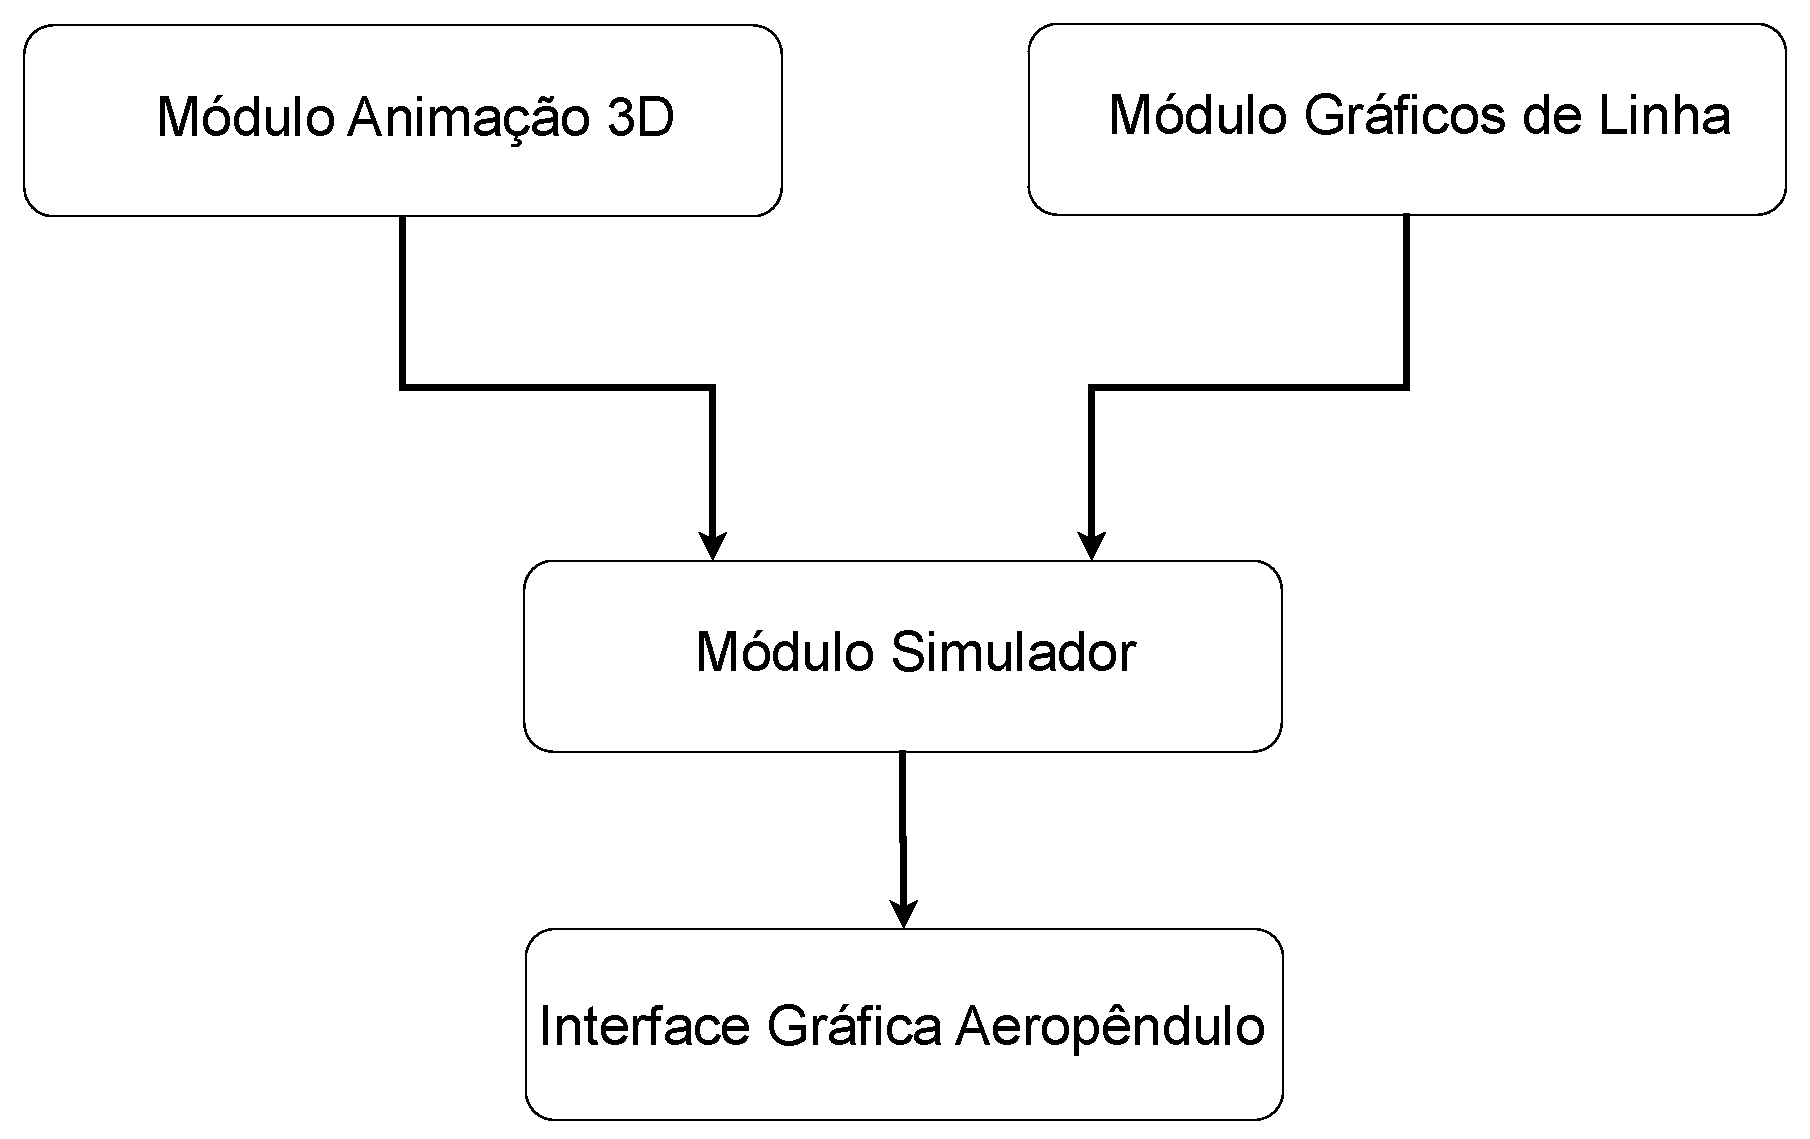
\includegraphics[width=0.55\textwidth, page=1]{Capitulos/3_hardware_softwares/3_figuras/arquitetura_simulador.pdf}}
        \vspace{0.2cm}
	\caption*{Fonte: elaborado pelo autor (2023).}
	\label{fig3:image_13}
\end{figure}


\newpage

O \textbf{Módulo Simulador}, código abaixo, recebe como parâmetro  o \textbf{Módulo Animação 3D} e o \textbf{Módulo Gráficos de Linha}, a partir disso  é implementada uma Classe Python usando a ideia de programação orientada a objetos para realizar a construção tanto da parte gráfica quanto do simulador 2D.

\vspace{0.5cm}

\begin{lstlisting}[language=python, numbers=left, label=python-example, captionpos=b, caption={Classe que implementa o Gêmeo Digital}]
import vpython as vp

# Modulos do Gemeo Digital desenvolvidos
from .interfaces.graficos_aeropendulo import GraficosInterface
from .interfaces.animacao_aeropendulo import AnimacaoAeropenduloInterface
from .interfaces.simulador import SimuladorInterface


class Simulador(SimuladorInterface):
    def __init__(
            self, graficos: GraficosInterface,
            animacao_aeropendulo: AnimacaoAeropenduloInterface) -> None:
        self.t = 0
        self.t_ant = 0
        self.ts = 0
        self.theta_rad = 0
        self.theta_rad_ant = 0
        self.dtheta_rad = 0
        # Instanciando um objeto AeropenduloAaeropendulo()
        self.animacao_aeropendulo = animacao_aeropendulo

        # Instanciando um objeto para plotagem dos graficos
        # dinamicos dos estados do Aeropendulo
        self.g = graficos
        self.graf, self.plot1, self.plot2 = self.g.graficos()  # noqa

    def grau2rad(self, graus):
        return (graus)*(vp.pi/180.0)

    def rotate(self, angle) -> None:
        self.valor_angle = self.grau2rad(angle)
        self.animacao_aeropendulo.aeropendulo.rotate(
            axis=vp.vec(0, 0, 1),
            angle=self.valor_angle,
            origin=vp.vec(0, 5.2, 0))
        self.animacao_aeropendulo.set_posicao_helice(self.valor_angle)

    def atualizar_estados(self, t, theta, ref):
        self.t = t
        self.ts = self.t - self.t_ant
        self.theta_rad = self.grau2rad(theta)
        try:
            self.dtheta_rad = (
                self.theta_rad - self.theta_rad_ant
                )/self.ts
        except Exception as exception:
            print(exception)

        # Atualiza o angulo do Aeropendulo
        self.animacao_aeropendulo.aeropendulo.rotate(
                        axis=vp.vec(0, 0, 1),
                        angle=self.dtheta_rad*self.ts,
                        origin=vp.vec(0, 5.2, 0))

        # Animacao da dinamica da Helice
        self.animacao_aeropendulo.update_helice(self.dtheta_rad, self.ts)

        # print(x[1] + interface.valor_angle)
        # Grafico do angulo.
        self.plot1.plot(t, theta)
        # Grafico do sinal de referencia
        self.plot2.plot(t, ref)

        self.t_ant = t
        self.theta_rad_ant = self.theta_rad

\end{lstlisting}

Para atualizar a dinâmica do braço do Aeropêndulo do Gêmeo Digital, a classe \textbf{Simulador} é importada no outro software, seção \ref{interface_graica} que implementa a comunicação com o protótipo e obtêm os estados do sistema real, assim é possível atualizar o Gêmeo Digital com dados reais do braço do Aeropêndulo.

Logo, o código desenvolvido para implementar o Gêmeo Digital deve ser importado no código que implementa a Interface Gráfica de Usuário, seção \ref{interface_graica}.

\subsection{Interface Gráfica para Configuração, visualização e aquisição de dados da Planta}
\label{interface_graica}

A interface gráfica consiste de um menu com diferentes opções de controle e visualização dos sinais do sistema e um conjunto de gráficos dinâmicos para visualizar os estados do sistema em tempo real. A figura \ref{fig3:image_14} mostra a interface do sistema. No entanto, além da parte visual existe a parte de aquisição e processamento de dados, em TI essa parte e chamada de Back-end, o projeto possui uma classe para realizar essa parte de aquisição e tratamento de dados, além de uma classe para detectar automaticamente o microcontrolador conectado a porta USB.

Para ser possível realizar os ensaios, modificação de parâmetros do sinal de referência e coletas de dados é preciso que o microcontrolador execute o firmware, subseção \ref{firmware}, desenvolvido especificamente para esse propósito, dessa forma, a interface gráfica, figura \ref{fig3:image_14}, conseguirá realizar o pre-processamentos dos dados e plotar os sinais nos gráficos e demais atualizações nos softwares.

\begin{figure}[!h]
	\centering
	\caption{Interface Gráfica.}
	\efbox{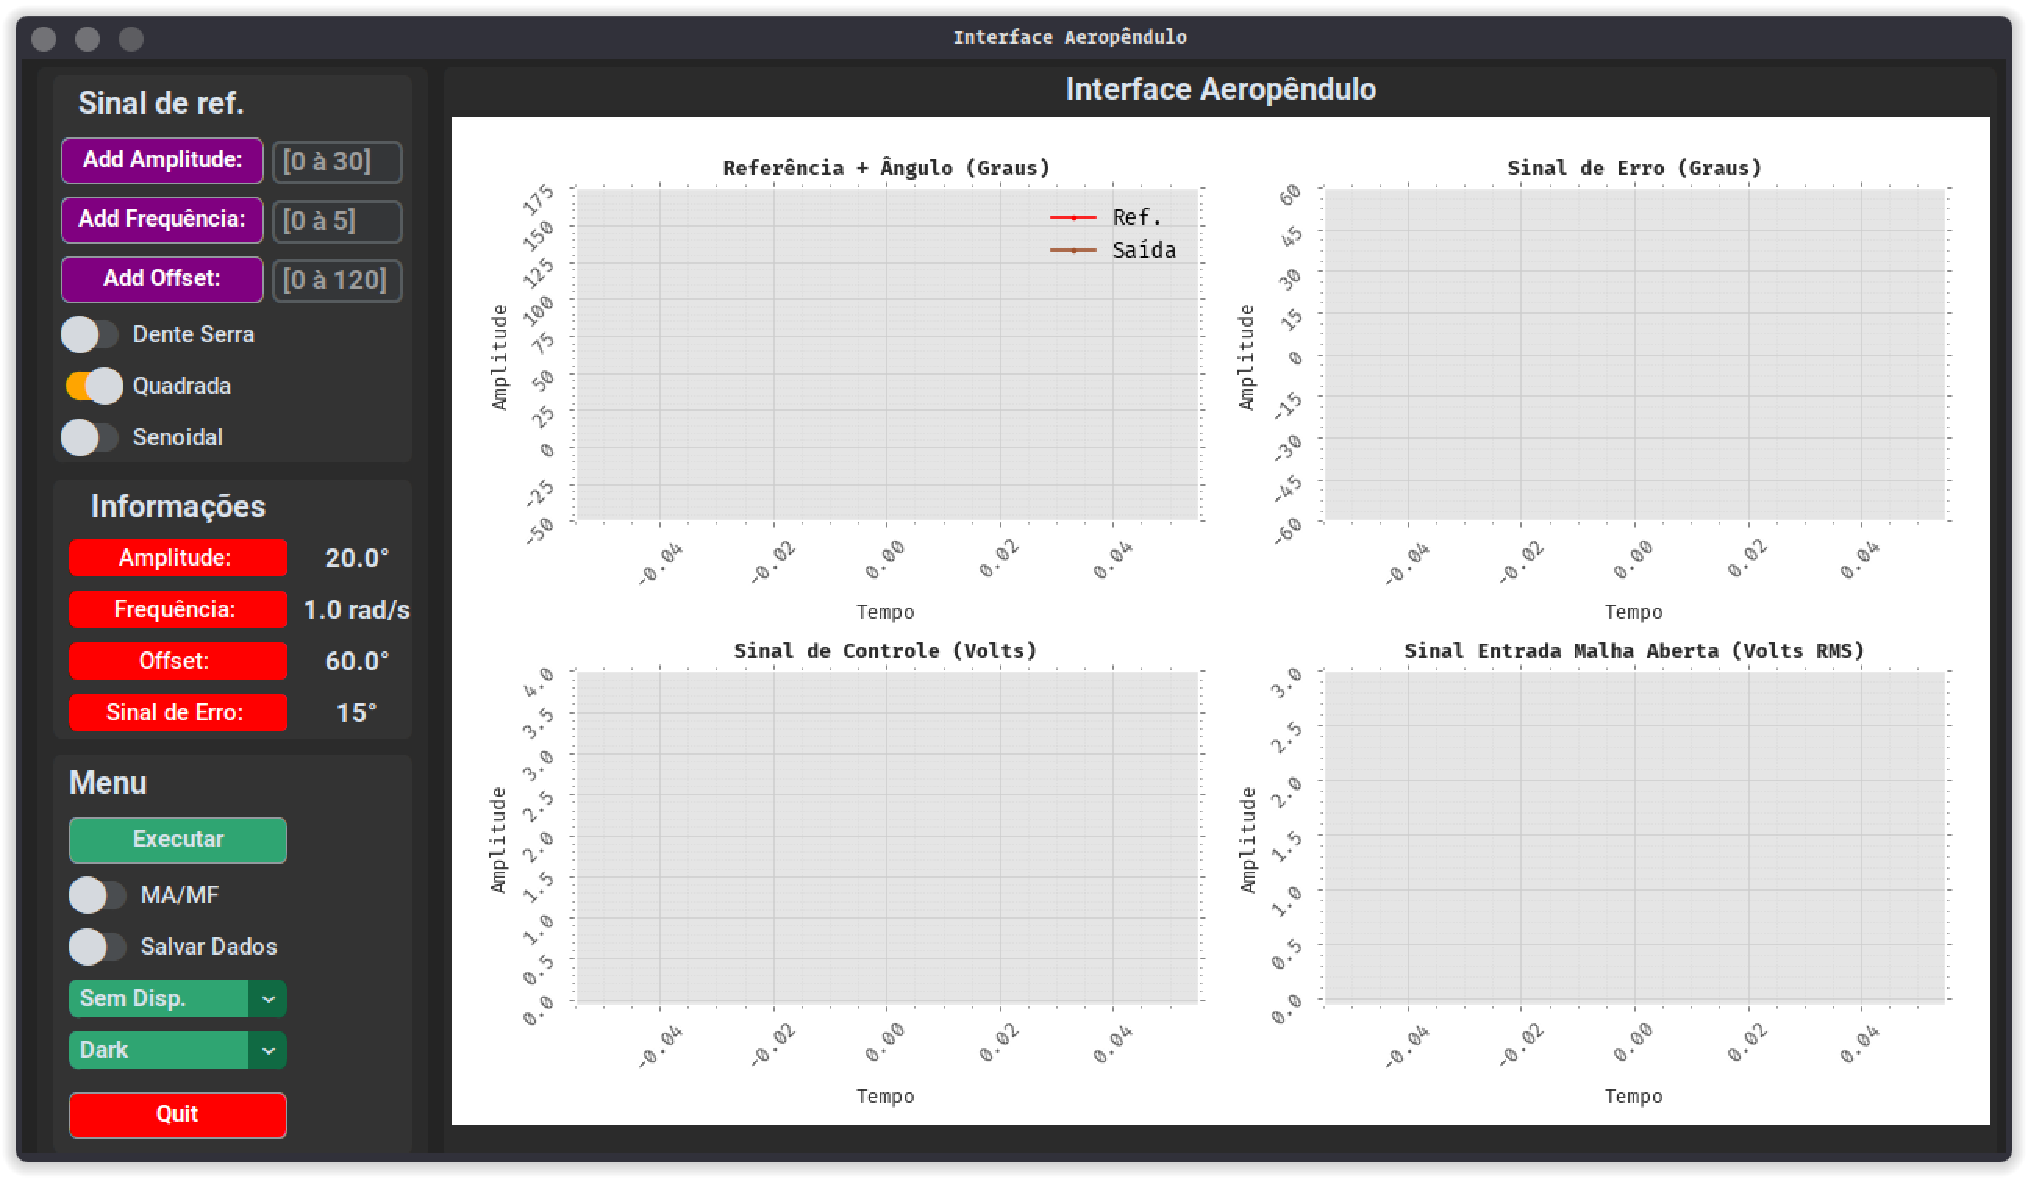
\includegraphics[width=0.9\textwidth]{Capitulos/3_hardware_softwares/3_figuras/interface.pdf}}
        \vspace{0.001cm}
	\caption*{Fonte: elaborado pelo autor (2023).}
	\label{fig3:image_14}
\end{figure}



O código a seguir realiza a importação de todos os módulos Python desenvolvidos tanto para a implementação da Interface Gráfica do Usuário quanto para o Gêmeo Digital. Com base nisso, foi elaborado um algoritmo que organiza adequadamente o funcionamento de ambos os softwares, viabilizando uma comunicação eficiente entre eles.

\vspace{0.5cm}

\begin{lstlisting}[language=python, numbers=left, label=py2, caption={Código que execulta a Interface Gráfica e o Gêmeo Digital.}]
import argparse
# Modulos da Interface Grafica de Usuario
from src_interface import InterfaceAeropendulo
from src_interface.graficos_sinais import GraficosSinais

# Modulos do Gemeo Digital
from simulador_aeropendulo.simulador import Simulador
from simulador_aeropendulo.graficos_aeropendulo import Graficos
from simulador_aeropendulo import AnimacaoAeropendulo

class RunInterface:
    def __init__(self) -> None:
        simular = self.get_args()
        self.runinterface(simular)

    def get_args(self) -> bool:
        parser = argparse.ArgumentParser()
        parser.add_argument(
            "-simular", "--Output",
            help="""Para habilitar o simulador, use a sintax:
                    python rungui.py -simular sim""")
        args = parser.parse_args()
        if args.Output == "sim":
            return True
        else:
            return False

    def runinterface(self, simular):
        if simular:
            simulador = Simulador(Graficos(), AnimacaoAeropendulo())
        else:
            simulador = None
        InterfaceAeropendulo(GraficosSinais,
                             simulador, baud_rate=115200,
                             amostras=80.0, tela_fixa=True)

if __name__ == "__main__":
    RunInterface()

\end{lstlisting}


Para roda a Interface Gráfica de Usuário juntamente com o Gêmeo Digital usa-se o seguinte comando no terminal estando dentro da pasta a partir do terminal:

\vspace{0.5cm}

\begin{lstlisting}[language=python]
python rungui.py -simular sim
\end{lstlisting}

Para roda apenas a Interface Gráfica de Usuário usa-se o seguinte comando no terminal:

\vspace{0.5cm}

\begin{lstlisting}[language=python]
python rungui.py
\end{lstlisting}



\subsubsection{Biblioteca CustomTkinter e Matplotlib}

Para o desenvolvimento da parte gráfica do software foi usado as bibliotecas CustomTkinter e Matplotlib, onde a biblioteca CustomTkinter implementa a estrutura de tela, botões, entradas de texto da aplicação e os módulos \textit{Matplotlib.pyplot} e \textit{Matplotlib.animation} possibilitam gerar gráficos em tempo real em conjunto com CustomTkinter.

Conforme \cite{customtkinter} explica no site oficial da biblioteca, "CustomTkinter é uma biblioteca de UI de desktop python baseada em Tkinter, que fornece widgets de aparência moderna e totalmente personalizáveis. Com CustomTkinter você terá uma aparência consistente em todas as plataformas de desktop (Windows, macOS, Linux)."

De acordo com \cite{matplotlib}, "Matplotlib é uma biblioteca abrangente para criar visualizações estáticas, animadas e interativas em Python. Matplotlib torna as coisas simples fáceis e as difíceis possíveis."

\subsubsection{Biblioteca PySerial, NumPy e Pandas}
Já para implementar o Back-end foram utilizadas as bibliotecas PySerial, NumPy e Pandas. Sendo que a biblioteca PySerial tem por finalidade realizar a comunicação entre o computador e o microcontrolador usando o protocolo seial via entrada USB, já o NumPy teve sua aplicação no processo de criação das matrizes contendo os dados lidos pela PySerial, por fim, para salvar os dados de ensaio foi usada a biblioteca Pandas, sendo salvos no formato CSV.

Conforme \cite{pyserial}, "A biblioteca PySerial possibilita a comunicação serial entre o computador e o microcontrolador usando conexão USB, Este módulo encapsula o acesso à porta serial. Ele fornece backends para Python rodando em Windows, OSX, Linux, BSD (possivelmente qualquer sistema compatível com POSIX) e IronPython. O módulo denominado “serial” seleciona automaticamente o backend apropriado."

% \citeonline[p.~11]{numpy_opl}   - Exemplo

De acordo com \cite{numpy_opl}, "O NumPy, uma biblioteca essencial para Python, oferece recursos robustos para realizar cálculos numéricos, sendo seu elemento central o ndarray, também conhecido como tensor. O ndarray se destaca por sua homogeneidade, exigindo que todos os elementos pertençam ao mesmo tipo, em contraste com as listas Python."

Segundo \cite{pandas}, site oficial da ferramenta, "pandas é uma ferramenta de análise e manipulação de dados de código aberto rápida, poderosa, flexível e fácil de usar, construído sobre a linguagem de programação Python."


\subsubsection{Descrição das partes da interface gráfica}

Nessa subseção será detalhado as partes do software, a figura \ref{fig3:image_15} está enumerando as partes e suas descrições estão logo abaixo.

\begin{figure}[!h]
	\centering
	\caption{Partes da Interface Gráfica.}
	\efbox{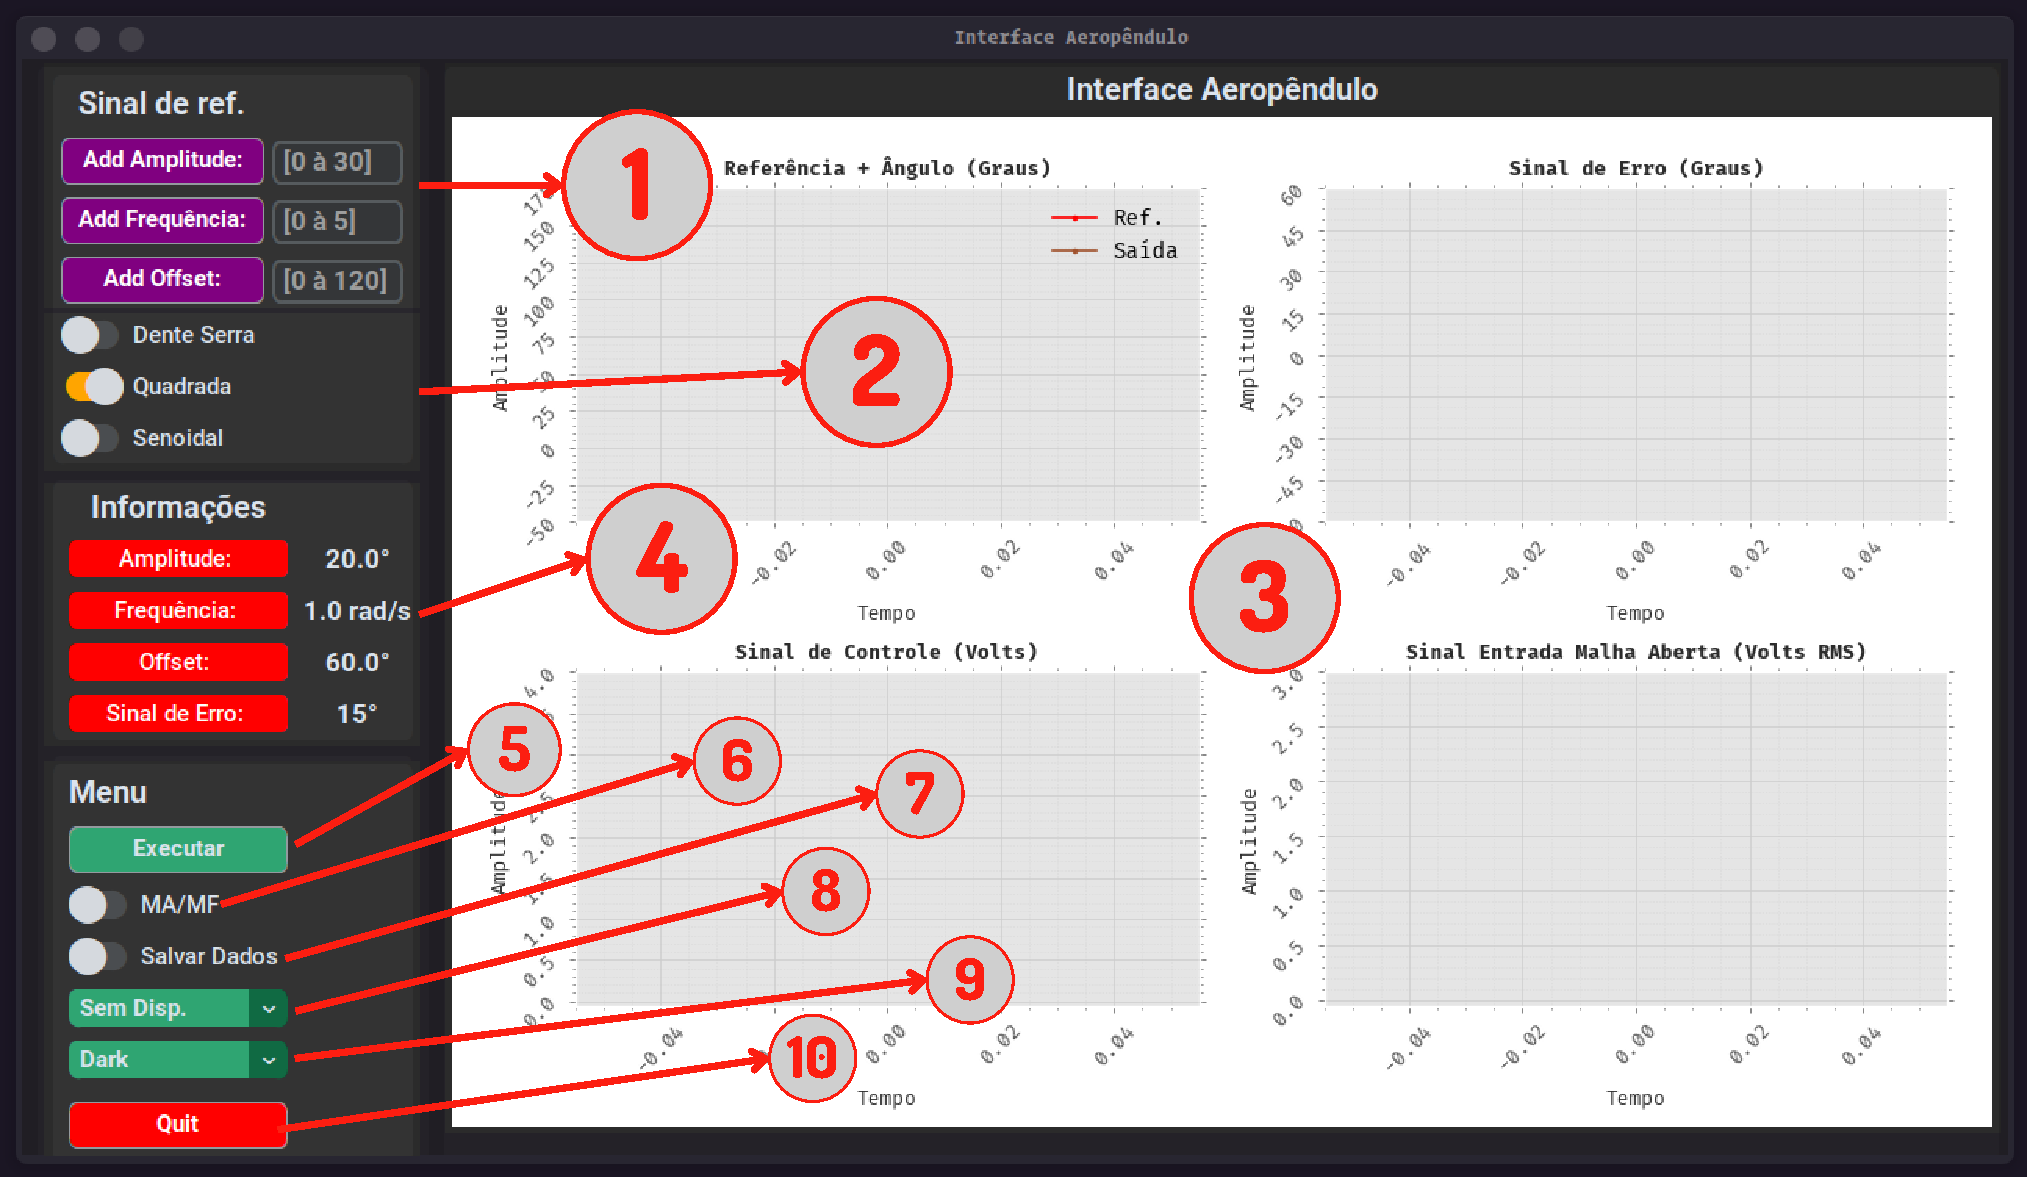
\includegraphics[width=0.95\textwidth]{Capitulos/3_hardware_softwares/3_figuras/interface_partes.pdf}}
	\caption*{Fonte: elaborado pelo autor (2023).}
	\label{fig3:image_15}
\end{figure}



\subsubsection*{\textit{Item 1: Sinal de Referência}}

Essa parte do software configura os sinais de referência aplicado ao sistema em malha fechada.


\begin{itemize}
        \setlength{\itemsep}{-2pt}
	\item  \textbf{Add Amplitude:} Configura a amplitude do sinal aplicado a entrada do sistema;
        \item  \textbf{Add Frequência:} Configura a frequência do sinal aplicado a entrada do sistema;
        \item  \textbf{Add Offset:} Configura a amplitude do offset, ponto de equilíbrio, aplicado a entrada do sistema.
\end{itemize}


\subsubsection*{\textit{Item 2: Seleção do Sinal de referência}}


\begin{itemize}
        \setlength{\itemsep}{-2pt}
	\item \textbf{Onda Serra:} Ao selecionar essa opção o sinal aplicado ao sistema será um dente de serra com as configurações de amplitude, frequência e offset conforme configurado nos três primeiros sub itens;
        \item \textbf{Quadrada:} Ao selecionar essa opção o sinal aplicado ao sistema será uma onda quadrada com as configurações de amplitude, frequência e offset conforme configurado nos três primeiros sub itens.;
        \item \textbf{Senoidal:} Ao selecionar essa opção o sinal aplicado ao sistema será uma onda senoidal com as configurações de amplitude, frequência e offset conforme configurado nos três primeiros sub itens.
\end{itemize}

\subsubsection*{\textit{Item 3: Gráficos}}

\begin{itemize}
        \setlength{\itemsep}{-2pt}
	\item \textbf{Gráficos:} Nesse item que são plotados os gráficos dos estados do sistema em tempo real.
\end{itemize}

\subsubsection*{\textit{Item 4: Informações}}

\begin{itemize}
        \setlength{\itemsep}{-2pt}
	\item \textbf{Amplitude:} Mostra a valor da amplitude do sinal de referência;
        \item \textbf{Frequência:} Mostra a valor da frequência do sinal de referência;\\
        \item \textbf{Offset:} Mostra a valor de offset aplicado ao aeropêndulo, esse valor é adicionado ao sinal de referência, dessa forma o sinal de referência varia em torno de um ponto de equilíbrio;
        \item \textbf{Sinal de Erro:} Mostra a valor do sinal de erro em tempo real.
\end{itemize}


\subsubsection*{\textit{Item 5: Menu}}

\begin{itemize}
        \setlength{\itemsep}{-2pt}
	\item \textbf{Executar:} Inicializa o ensaio, para isso é preciso que o microcontrolador esteja conectado ao computador.
\end{itemize}


\subsubsection*{\textit{Item 6: Menu}}

\begin{itemize}
        \setlength{\itemsep}{-2pt}
	\item \textbf{MA/MF:} Comuta entre o sistema em malha aberta e malha fechada.
\end{itemize}


\subsubsection*{\textit{Item 7: Menu}}

\begin{itemize}
        \setlength{\itemsep}{-2pt}
	\item \textbf{Salvar Dados:} Quando está ativado os dados são salvos em um arquivo CSV com data, hora, minuto e segundo do instante do salvamento, isso facilita que diferentes ensaios sejam realizados sem que os dados do anterior seja sobrescrito.
\end{itemize}


\subsubsection*{\textit{Item 8: Menu }}

\begin{itemize}
        \setlength{\itemsep}{-2pt}
	\item \textbf{Selecionar Dispositivo:} A aplicação detecta todos os microcontroladores conectados no computador e permite que o usuário realize a seleção do dispositivo desejado para realizar o ensaio.
\end{itemize}


\subsubsection*{\textit{Item 9: Menu}}

\begin{itemize}
        \setlength{\itemsep}{-2pt}
	\item \textbf{Selecionar Tema:} O software possui tema escuro e claro e essa opção permite que o usuário selecione entre essas duas opções.
\end{itemize}


\subsubsection*{\textit{Item 10: Menu}}

\begin{itemize}
        \setlength{\itemsep}{-2pt}
	\item \textbf{Quit:} Botão responsável por fechar a aplicação.
\end{itemize}



\subsection{Firmware do microcontrolador}
\label{firmware}
O firmwawe para o aeropêndulo foi desenvolvido a partir de bibliotecas, cada biblioteca tem sua funcionalidade, com isso o projeto se torna mais flexível, podendo ser atualizado e incrementado a medida que o projeto se torne mais robusto. 

Para desenvolver o firmware, utilizamos a ferramenta de plataforma cruzada PlatformIO. Essa ferramenta foi criada com o propósito de centralizar o desenvolvimento de firmware, possibilitando a programação para diversos microcontroladores, como o ESP32, a Família do Arduino, STM32 e muitos outros. Isso torna o projeto ainda mais flexível e versátil. A arquitetura é descrita na Figura \ref{fig3:image_16}.


\begin{figure}[!h]
	\centering
	\caption{Arquitetura do Firmware do Aeropêndulo.}
	\efbox{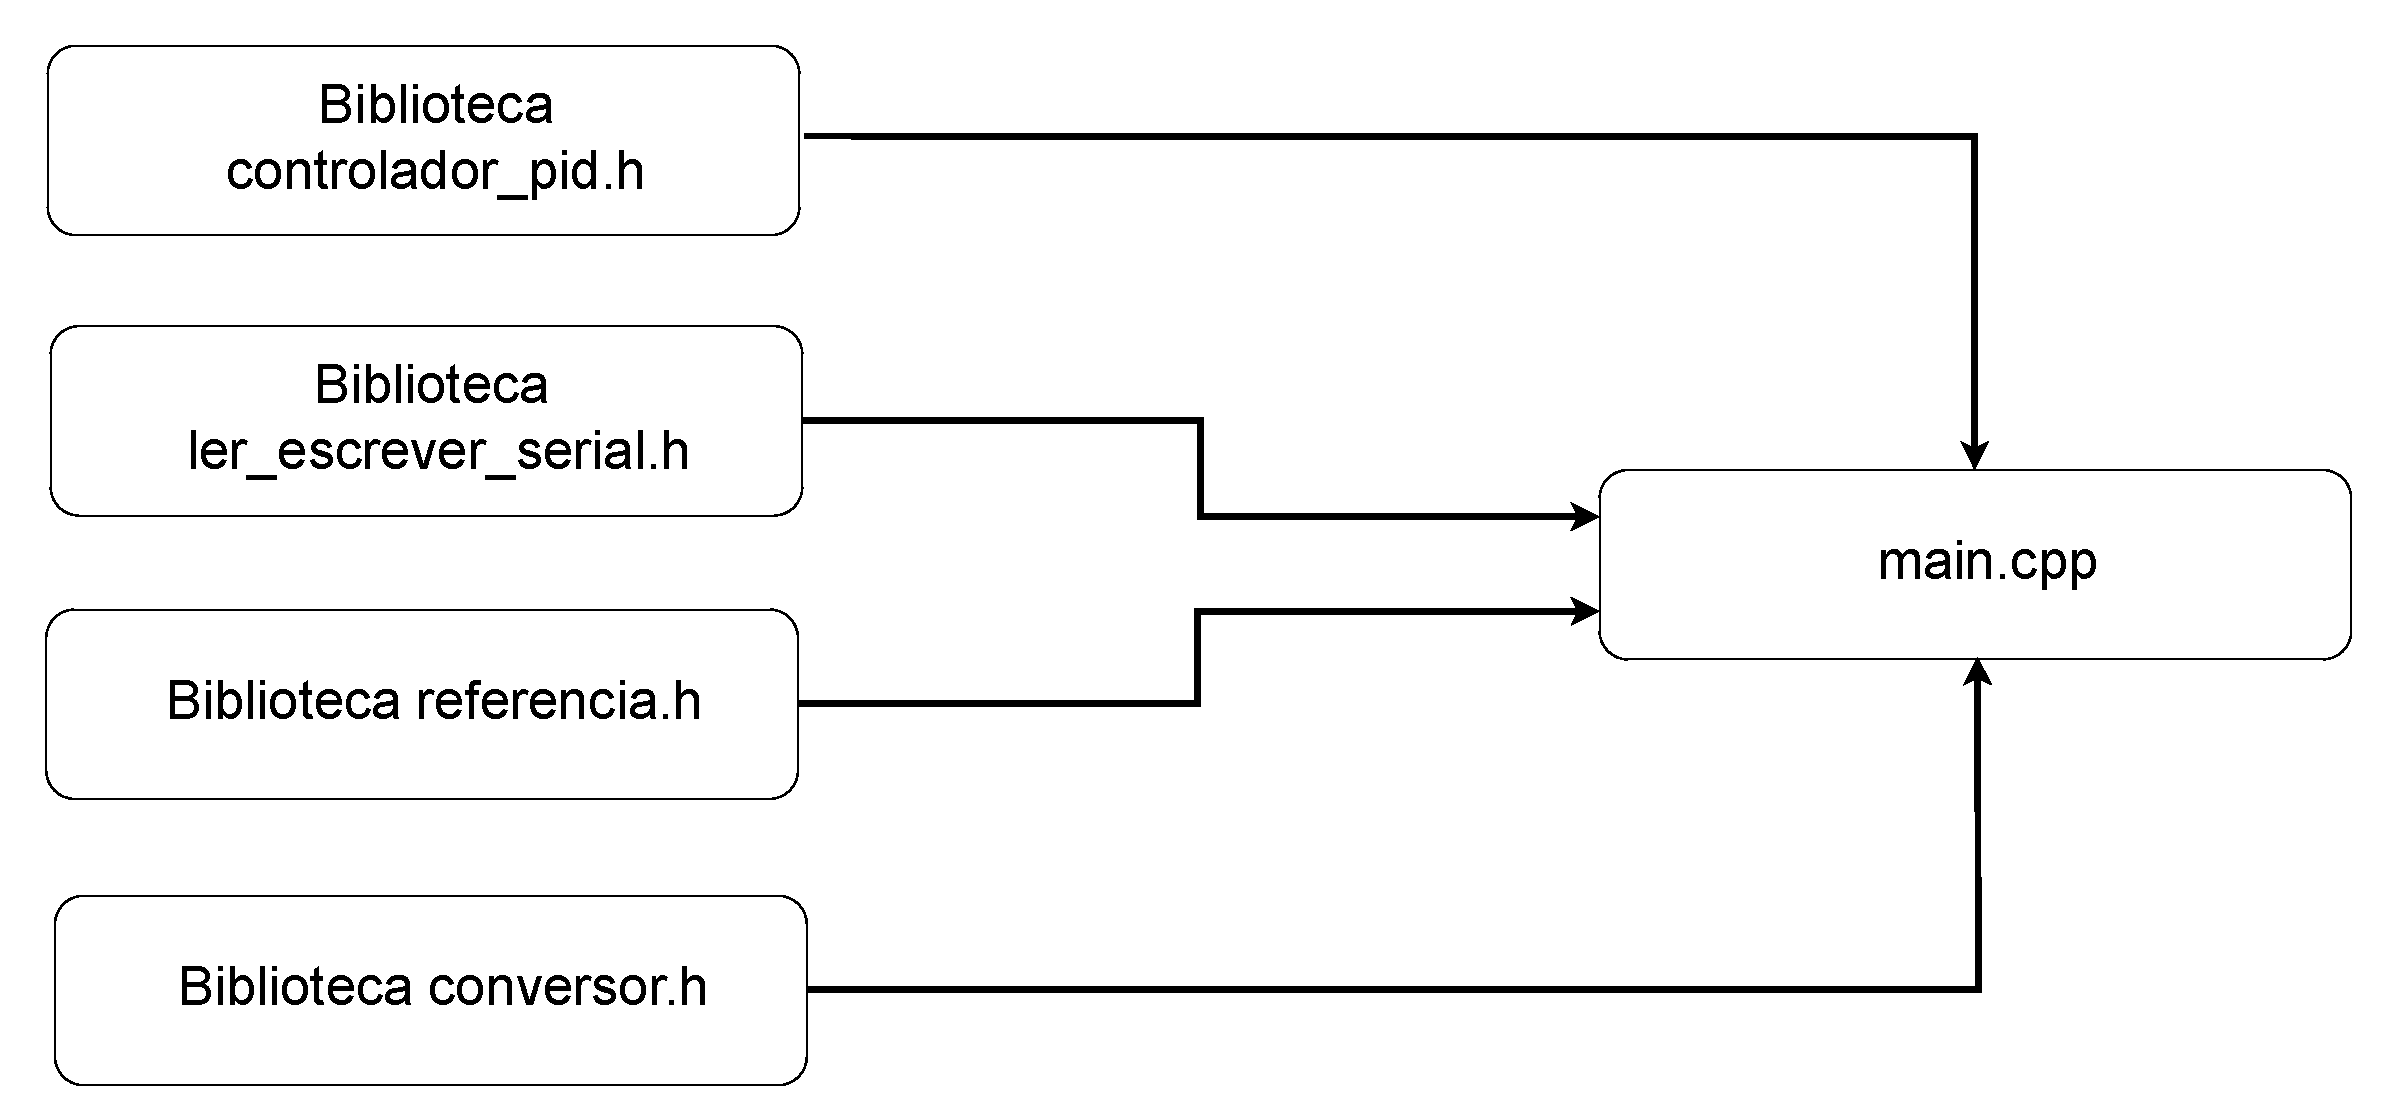
\includegraphics[width=0.8\textwidth]{Capitulos/3_hardware_softwares/3_figuras/arquitetura_firmware.pdf}}
	\caption*{Fonte: elaborado pelo autor (2023).}
	\label{fig3:image_16}
\end{figure}


\subsubsection{Biblioteca ler\_escrever\_serial}

Para realizar a configuração dos parâmetros do sinal de referência em tempo real e o envio dos sinais do sistema via porta serial foi desenvolvido a biblioteca ler\_escrever\_serial, assim, a parte de recebimento e envio de dados do sistema fica centralizada permitindo sua melhoria e modificação sem interferir na lógica do código principal "main.cpp".

\subsubsection{Biblioteca referencia}

O sistema em malha fechada possui uma entrada de referência que o controlador tem por finalidade rastrear, para tornar o projeto do firmware mais legível criou-se o módulo referencia.h em que implementa inicialmente três sinais de referência com a possibilidade de configurar os parâmetros de Amplitude, frequência e offset, sendo esses sinais Onda Quadrada, Onda Senoidal e Onda Dente de Serra. Caso, observe-se a necessidade de outros sinais, basta adicionar a biblioteca.

\subsubsection{Biblioteca conversor}


Essa biblioteca possui uma classe cpp com métodos de conversões de diferentes grandezas, a primeira conversão é do sinal de um potenciômetro para angulo, o segundo método converte o sinal de controle para ciclos PWM, o terceiro método converte de grau para radiano e o quarto de radiano para grau.

\subsubsection{Biblioteca controlador\_pid}

Essa biblioteca implementa uma classe cpp para o controlador PID para ser empregado no protótipo quando selecionado a opção em malha fechada na interface gráfica.


\subsubsection{Arquivo Principal mian.cpp}

A ferramenta PlatformIO possui uma estrutura que permite a criação de bibliotecas e um arquivo main.cpp que implementa a lógica do algorítimo, com isso é possível incluir as bibliotecas desenvolvidas e criar o algorítimo para o que se deseja.


Ou seja, o firmaware para o projeto possui várias funcionalidades que passam pela implementação do sinal de referência, leitura do sensor potenciômetro, envio e recebimento de dados via porta serial e implementação do controlador.

Por fim, com o firmware finalizado, o envio para o ESP32 é realizado usando o PlatfrmIO que concretiza a compilação e escrita no microcontrolador via porta serial.


\section{Fluxograma do Laboratório Virtual}
\label{flu_lab_virtual}
Dado o caráter multifacetado deste projeto, a compreensão das interações entre seus diversos subsistemas pode apresentar desafios significativos. Com o propósito de simplificar e aprofundar esse processo de compreensão, a figura \ref{fig3:image_17} oferece uma representação visual por meio de um diagrama de blocos que esclarece as dinâmicas entre os distintos subsistemas desenvolvidos. Essa abordagem contribui para facilitar o entendimento holístico do sistema na totalidade, proporcionando um recurso valioso para pesquisadores futuros que desejam explorar e aprimorar este laboratório.


\begin{figure}[!h]
	\centering
	\caption{Diagrama do Laboratório Virtual.}
	\efbox{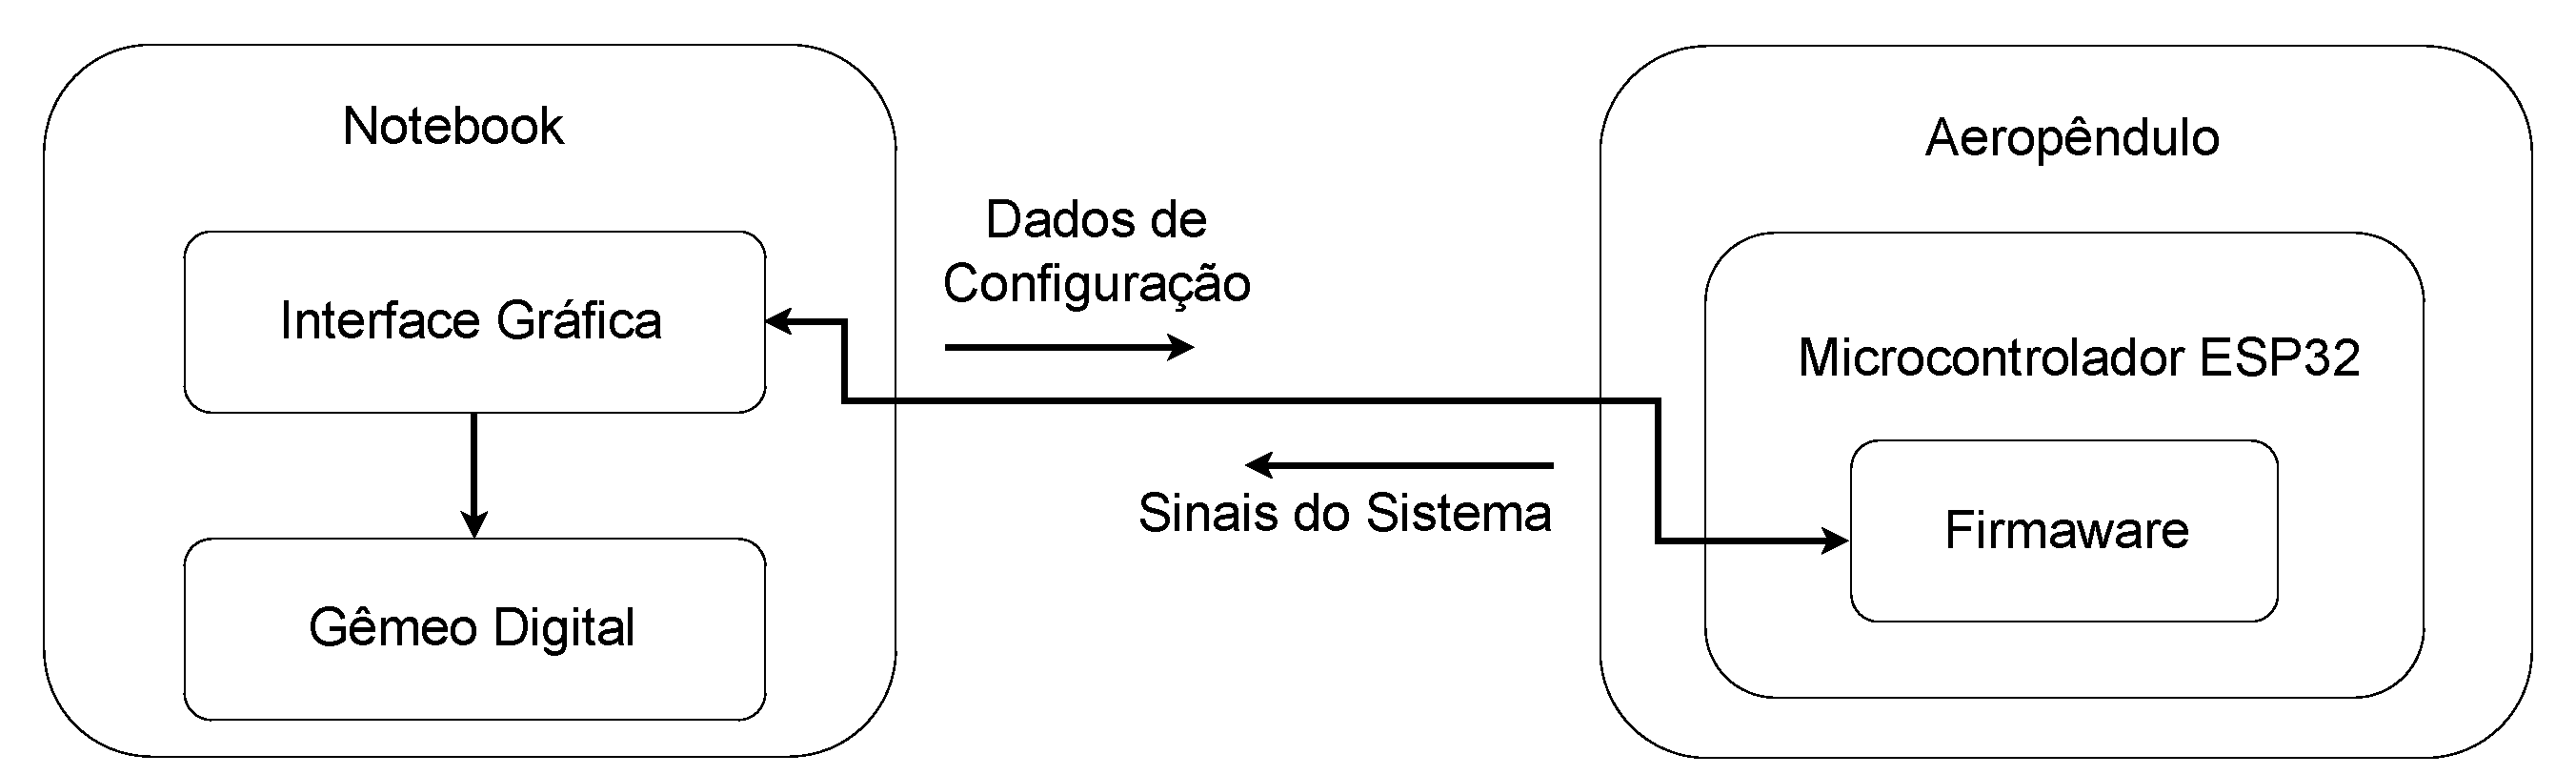
\includegraphics[width=1.0\textwidth]{Capitulos/3_hardware_softwares/3_figuras/diagrama_ecossistema.pdf}}
	\caption*{Fonte: elaborado pelo autor (2023).}
	\label{fig3:image_17}
\end{figure}




\chapter{Resultados e Discussões}
\label{cap_3}

\section{Desenvolvimento do Protótipo e Softwares}

Os sistemas propostos tanto físico quanto softwares foram desenvolvidos de forma exitosa, os procedimentos para a implementação se deu a partir de uma pesquisa bibliográfica e criativa, tendo como resultado o protótipo, figura \ref{fig3:image_01}, e os softwares, figuras \ref{fig3:image_13_1}, \ref{fig3:image_14} e \ref{fig3:image_16}.


\section{Identificação de sistema aplicado ao Aeropêndulo}
\label{indentificacao}

Com os subsistemas desenvolvidos, foram realizados alguns testes para validá-los, assim, o primeiro teste aplicado ao conjunto se tratou da identificação de sistemas. Após a identificação realizou-se uma simulação de modo a comparar o sinal de saída real com o simulado, com o intuito de analisar a dinâmica do sistema identificado e poder comparar com o sistema real.

A partir do ecossistema desenvolvido para o projeto é possível usá-lo para estudar diferentes aspectos na área de sistemas de controle, uma delas e a identificação de sistemas, para esse trabalho o método em questão foi usado para avaliar o correto funcionamento projeto. Desa forma, o trabalho \cite{tcc_klarissa_ufpa} foi usando como base teórica para implementar o método.


\subsubsection{Aplicação do Sinal PRBS na Entrada do Sistema}

O sinal PRBS aplicado a entrada do sistema em malha aberta foi gerado no microcontrolador e convertido em sinal PWM para ser aplicado a entrada do Driver L298N, subseção \ref{driver_l298n}, seus parâmetros foram definidos com uma amplitude de 0,3V, frequência fundamental de 0,4Hz e período de amostragem de 0,02 segundos, além disso, aplicou-se um offset de 1V (Ponto de operação), com isso, obteve-se o sinal PRBS de entrada mostrado na figura \ref{fig3:image_16}.


\begin{figure}[!h]
	\centering
	\caption{Sinal PRBS de entrada.}
	\efbox{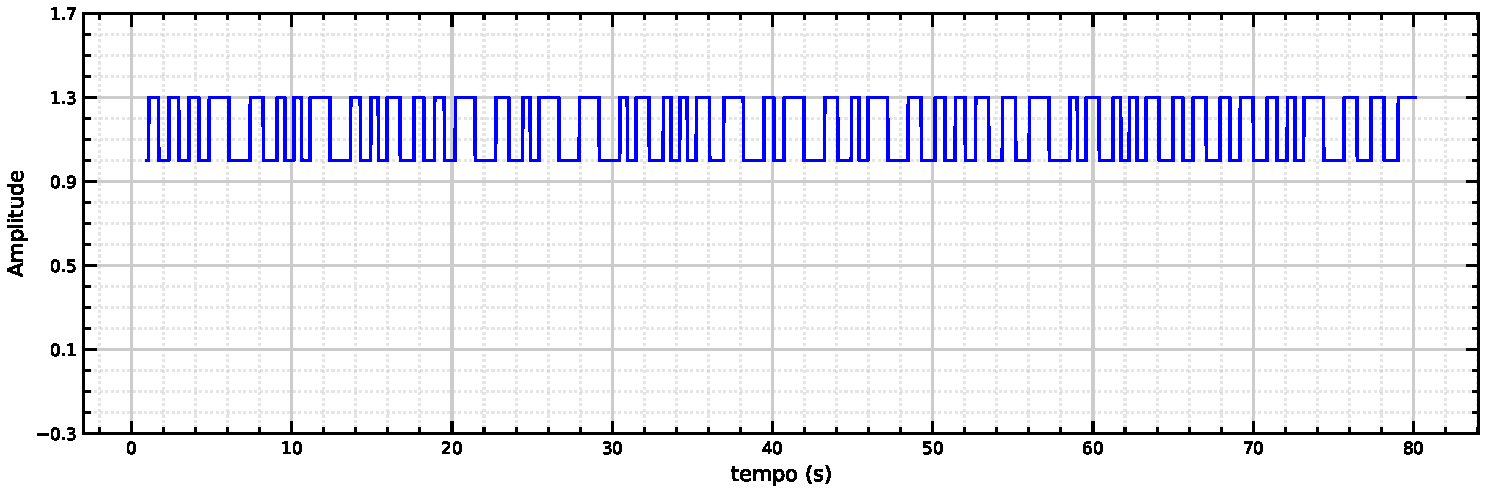
\includegraphics[width=1\textwidth]{Capitulos/3_1_resultados_discurcao/3_figuras/sinal_prbs_entrada_com_offset.pdf}}
	\caption*{Fonte: elaborado pelo autor (2023).}
	\label{fig3:image_18}
\end{figure}



\subsubsection{Sinal de Saída Gerado a Partir do Sinal PRBS de Entrada}

Para a obtenção do sinal de saída, que representa o ângulo do braço do aeropêndulo, foi empregado um método no qual um sinal PRBS foi aplicado à entrada do sistema. Para medir o ângulo, sinal de saída, utilizou-se um potenciômetro como sensor, cujas extremidades foram conectadas ao 3.3V e GND do ESP32. O terceiro fio do potenciômetro foi conectado a uma porta analógica do ESP32, permitindo, assim, a conversão da variação de tensão em valores angulares. A figura \ref{fig3:image_19} exibe o sinal de saída de um ensaio.

\begin{figure}[!h]
	\centering
	\caption{Sinal PRBS de saída.}
	\efbox{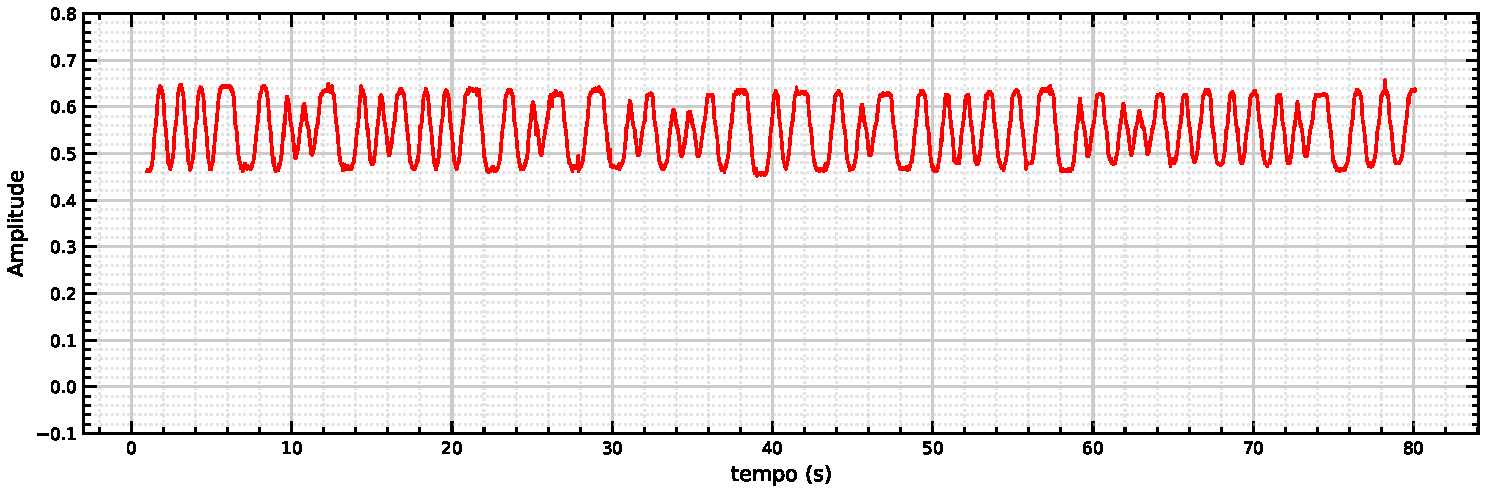
\includegraphics[width=1\textwidth]{Capitulos/3_1_resultados_discurcao/3_figuras/sinal_saida_com_offset.pdf}}
	\caption*{Fonte: elaborado pelo autor (2023).}
	\label{fig3:image_19}
\end{figure}

\subsection{Identificação Usando Mínimos Quadrados}


Para realizar a identificação de sistemas deve-se retirar os offsets tanto do sinal de entrada quanto para o de saída, com essa etapa realizada, deve-se separar dois conjuntos de dados para identificação e validação do modelo proposto, tanto para o sinal de entrada quanto para o de saída. Foi usando 60\% dos dados para identificação de 40\% para validação.

\subsubsection{Passos para realização da identificação}


\noindent\textit{Passo 1:} Obter dados Entrada/Saída do sistema;\\
\textit{Passo 2:} Dividir dados entre identificação e validação;\\
\textit{Passo 3:} Definir a Função de Transferência;\\
\textit{Passo 4:} Definir a matriz de regressão;\\
\textit{Passo 5:} Encontrar o vetor de coeficientes pela formulação de mínimos quadrados;\\
\textit{Passo 6:} Substituir os coeficientes na função de transferência escolhida anteriormente;\\
\textit{Passo 7:} Validar o modelo do sistema a partir de dados reais.\\

% O primeiro passo que deve ser realizado é escrever a estrutura da função de transferência proposta, dessa forma a equação \ref{eq3:eq1} foi a estrutura escolhida para modelar o sistema usando uma função de transferência de segunda ordem.

\subsubsection{Identificação Usando Função de Transferência Discreta de Segunda, Quinta e Décima Ordem}

Para realizar o cálculo numérico usando a base de dados do ensaio foi usando a linguagem de programação Python, que possui um conjunto de bibliotecas que facilita o implementação dos cálculos. Após obter os dados de ensaio, os passos seguintes foram desenvolvidos em um Script Python, sendo o primeiro passo a importação das bibliotecas, como mostra a célula de código abaixo.

\vspace{0.5cm}

\begin{lstlisting}[language=python, numbers=left, label=py3, caption={Importação das Bibliotecas usadas para identificação de sistemas.}]
import numpy as np 
import matplotlib.pyplot as plt
import pandas as pd
import control as ct
\end{lstlisting}

No segundo passo foi feito o carregamento dos dados de ensaio PRBS e realizada a separação entre dados de identificação e validação, para isso foi usado a biblioteca Pandas em conjunto com a biblioteca NumPy que possibilita carregar dados de diferentes formatos e manipulá-los, os dados de ensaio foram salvos em formato CSV (Comma-separated values), o código para realizar o carregamento dos dados e a separação é mostrado na célula de código abaixo.

\vspace{0.5cm}

\begin{lstlisting}[language=python, numbers=left, label=py4, caption={Carregando os dados do ensaio e realizando pré-processamento.}]
file = "caminho completo dos  dados/arquivo_9_9_2023_13_33_24.csv"
dados_malha_aberta_prbs = pd.read_csv(file, header=None, sep=',').values
dados_malha_aberta_prbs[0][0] = 0.0
dados_malha_aberta_prbs

# Variaveis contendo os dados de tempo, entrada e saida
tempo = np.array(dados_malha_aberta_prbs[:,7])
sinal_prbs_entrada  = np.array(dados_malha_aberta_prbs[:,6])
sinal_saida = np.array(dados_malha_aberta_prbs[:,2])

# Convertendo o sinal de Graus para Radianos
sinal_saida = np.squeeze(np.deg2rad(sinal_saida))
tempo = tempo - min(tempo)
\end{lstlisting}


Além disso, é necessário remover as primeiras amostras por conter o transitório do sistema e retirar os offsets dos sinais de entrada e saída, o que é feito na célula de código abaixo. A figura \ref{fig3:image_20} exibe os gráficos dos sinais de entrada/saída, podemos observar que os sinais estão centralizados em zero e não possui transitório no início do sinal.

\vspace{0.5cm}


\begin{lstlisting}[language=python, numbers=left, label=py3, caption={Centralizando os sinais de entrada e daída em zero.}]
u1 = sinal_prbs_entrada[50:] - np.mean(sinal_prbs_entrada[50:])
yout = sinal_saida[50:] - np.mean((sinal_saida[50:]))
t = tempo[50:]
\end{lstlisting}

\begin{figure}[!h]
	\centering
	\caption{Dados de identificação e validação do modelo.}
	\efbox{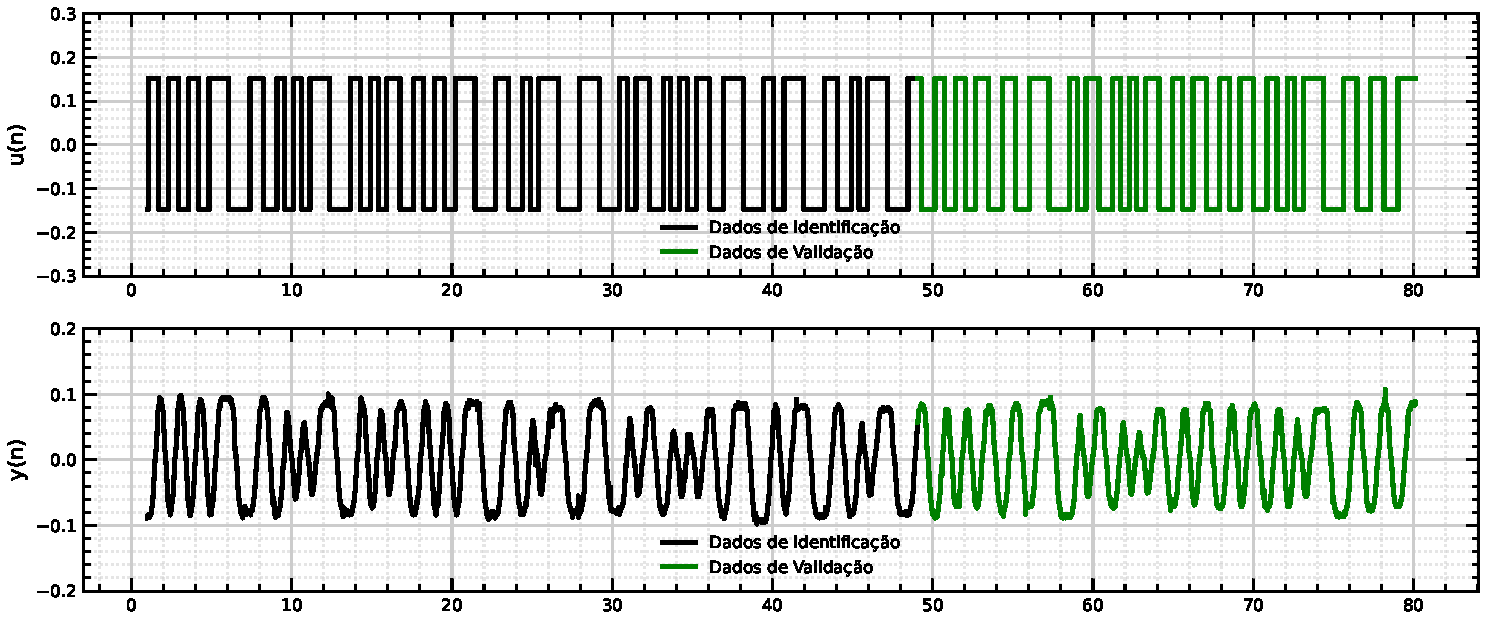
\includegraphics[width=1\textwidth]{Capitulos/3_1_resultados_discurcao/3_figuras/dados_traino_teste.pdf}}
	\caption*{Fonte: elaborado pelo autor (2023).}
	\label{fig3:image_20}
\end{figure}

Com os dados de ensaio pré-processados e prontos para aplicar a técnica de identificação, foi definida uma função de transferência discreta, essa função tem a finalidade de aproximar um modelo que satisfaça a dinâmica do aeropêndulo. Para um primeiro teste foi usada uma função de segunda ordem, como mostra a equação \ref{eq3:eq1}.

\begin{align}
    H(z) = \frac{b_1z^{-1}+b_2z^{-2}}
    {1+a_1z^{-1}+a_2z^{-2}} \label{eq3:eq1}
\end{align}

Para aplicar o método dos mínimos quadrados e obter os coeficientes da função de transferência de segunda ordem precisa-se ter as matrizes de regressão tando para os dados de entrada quanto para os de saída, o código abaixo cria o algorítimo necessário para se obter as matrizes a partir dos dados do ensaio.

\vspace{0.5cm}

\begin{lstlisting}[language=python, numbers=left, label=py3, caption={Estruturando os dados para aplicar o método dos mínimos quadrados.}]
# Matriz de regressao:
nb = 3; na = 2
ni = np.arange(na, Ni + na)
M = np.zeros((Ni, na + nb))

# Para regressores de y:
for l in np.arange(0, na):
  M[:, l] = yout[ni - l - 1]

# Para regressores de u:
for l in np.arange(0, nb):
  M[:, na + l] = u1[ni - l]

print(M.shape)
\end{lstlisting}

Com as matrizes de regressores definidas, foi realizada a aplicação do método dos mínimos quadrados, o que é exemplificado na célula de código abaixo, a biblioteca NumPy possibilita cálculos de álgebra matricial de forma rápida e simples.

\vspace{0.5cm}

\begin{lstlisting}[language=python, numbers=left, label=py3, caption={Método dos mínimos quadrados.}]
# Minimos quadrados
thetaA = np.linalg.inv(M.T @ M) @ M.T @ yout[ni]
thetaA
\end{lstlisting}

Para a função de transferência de segunda ordem escolhida, equação \ref{eq3:eq1}, em que possui dois coeficientes no numerador e 3 no denominador, dessa forma, os coeficientes obtidos ao aplicar o método de mínimos quadrados retorna em suas duas primeiras posições os coeficientes do numerador e o restante são os coeficientes do denominador, a partir dos coeficientes obtidos, pode-se definir a função de transferência discreta do sistema, isso é feito no Python usando a biblioteca Python-Control que permite realizar ensaios simulados a partir da função de transferência.

\vspace{0.5cm}

\begin{lstlisting}[language=python, numbers=left, label=py3, caption={Salvando os coeficientes em variáveis e obtendo a função de transferência.}]
a1, a2 = thetaA[:2]
b0, b1, b2 = thetaA[2:]

Ba = [b0 , b1, b2]
Aa = [1, -a1, -a2]

Hz = ct.tf(Ba, Aa, Ts)
\end{lstlisting}

Função de transferência discreta, \ref{eq3:eq2}, com os coeficientes obtidos a partir do método de mínimos quadrados, o período de amostragem é $dt = 0,019$  segundos.

\begin{align}
Hz = \frac{-0.002602 z^2 + 0.004962 z + 0.0163}{z^2 - 1.176 z + 0.1849} \label{eq3:eq2}
\end{align}


Para validar o modelo encontrado é preciso testar a função de transferência discreta usando os dados de entrada do ensaio real, com isso obtém-se os dados de saída da simulação, esse dado pode ser comparado com a saída do sistema real, caso ambos os gráficos aproximem suas dinâmicas pode-se concluir que o modelo corresponde com o sistema real, caso contrário é preciso definir uma nova função de transferência e realizar novamente o teste de validação.

A biblioteca Python-control possibilita simular a dinâmica de um sistema a partir da sua função de transferência discreta, podendo receber como argumento um vetor de entradas, como mostrado a célula de código abaixo.

\vspace{0.5cm}

\begin{lstlisting}[language=python, numbers=left, label=py3, caption={Obtendo a resposta forçada da função de transferência obtida.}]
_, yp = ct.forced_response(Hz, U=u1)
\end{lstlisting}

Ao plotar os gráficos de saída real e simulada tem-se como resultado a figura \ref{fig3:image_21}, é possível observar que a saída da simulação não corresponde de forma aceitável com a dinâmica do sinal de saída do sistema real, ou seja, o modelo não foi robusto o suficiente para identificar o sistema em questão.

\begin{figure}[!h]
	\centering
	\caption{Validação do modelo de segundo grau.}
	\efbox{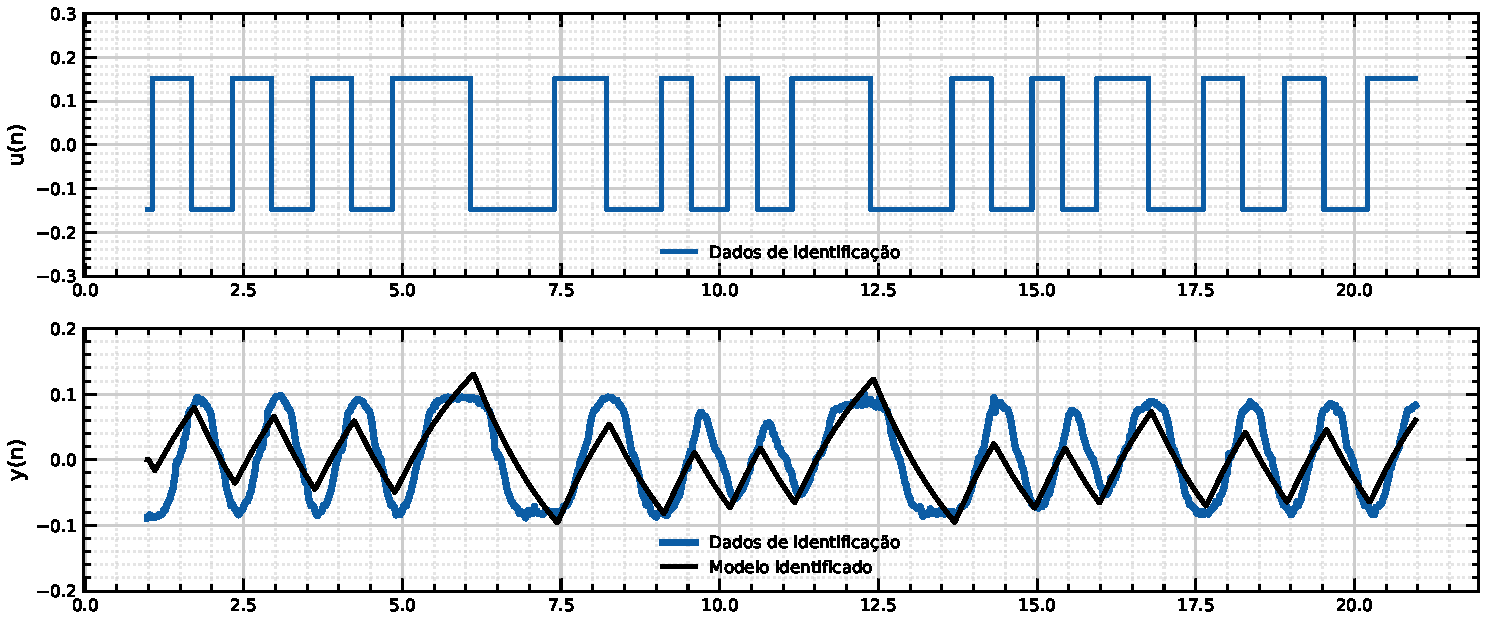
\includegraphics[width=1\textwidth]{Capitulos/3_1_resultados_discurcao/3_figuras/validacao_model_2grau.pdf}}
	\caption*{Fonte: elaborado pelo autor (2023).}
	\label{fig3:image_21}
\end{figure}

A partir de uma análise qualitativa, pode-se supor que o grau da função de transferência discreta escolhida não consegue aproximar a dinâmica real do aeropêndulo, dessa forma, foi realizado alguns testes e identificado que uma função de transferência discreta de décima ordem, equação \ref{eq3:eq3}, aproxima de forma aceitável o sistema real.

\begin{align}
H(z) = \frac{b_1z^{-1}+b_2z^{-2}+b_2z^{-3}+b_2z^{-4}}{1+a_1z^{-1}+a_2z^{-2}+a_2z^{-3}+a_2z^{-4}+a_2z^{-5}+a_2z^{-6}+a_2z^{-7}+a_2z^{-8}+a_2z^{-9}+a_2z^{-10}}\label{eq3:eq3}
\end{align}


Assim, foi ajustado o algorítimo para identificar o sistema a partir da estrutura da equação \ref{eq3:eq3}, o código abaixo gera as matrizes tanto para os regressores de entrada quanto para o de saída. 

\vspace{0.5cm}

\begin{lstlisting}[language=python, numbers=left, label=py3, caption={Estruturando os dados para aplicar o método dos mínimos quadrados.}]
# Matriz de regressao:
nb = 4
na = 10
ni = np.arange(na, Ni + na)
M = np.zeros((Ni, na + nb))

# Para regressores de y:
for l in np.arange(0, na):
  M[:, l] = yout[ni - l - 1]

# Para regressores de u:
for l in np.arange(0, nb):
  M[:,na+l] = u1[ni-l]

print(M.shape)
\end{lstlisting}


Com as matrizes de regressores ajustada para um sistema de décima ordem, foi realizada a aplicação do método dos mínimos quadrados.

\vspace{0.5cm}

\begin{lstlisting}[language=python, numbers=left, label=py3, caption={Método dos mínimos quadrados.}]
# Minimos quadrados
thetaA = np.linalg.inv(M.T @ M) @ M.T @ yout[ni]
thetaA
\end{lstlisting}

A equação \ref{eq3:eq3} possui 4 coeficientes no numerador e 10 no denominador, dessa forma, as quatro primeiras posições da variável  \textbf{thetaA} corresponde aos coeficientes do numerador e o restante aos coeficientes do denominador, a célula de código abaixo define a função de transferência usando a estrutura da equação \ref{eq3:eq3} e os coeficientes obtidos.

\vspace{0.5cm}

\begin{lstlisting}[language=python, numbers=left, label=py3, caption={Salvando os coeficientes em variáveis e obtendo a função de transferência.}]
a1, a2, a3, a4, a5, a6, a7, a8, a9, a10 = thetaA[:10]
b0, b1, b2, b3 = thetaA[10:]

Ba = [b0 , b1, b2, b3]
Aa = [1, -a1, -a2, -a3, -a4, -a5, -a6, -a7, -a8, -a9, -a10]

Hz = ct.tf(Ba, Aa, Ts)
\end{lstlisting}

Assim, obtém-se a função de transferência discreta, equação \ref{eq3:eq4}, com os valores encontrado a partir do método de mínimos quadrados, com período de amostragem de $dt = 0,02$ segundos.

\begin{align}
Hz = \frac{-0.0029 z^3 + 0.0023z^2 + 0.0016 z + 0.0097}{z^{10} - 0.9 z^9 - 0.3 z^8 - 0.014 z^7 + 0.13 z^6 + 0.15 z^5 + 0.012 z^4 - 0.05 z^3 - 0.12 z^2 - 0.02 z + 0.15} \label{eq3:eq4}
\end{align}

Por fim, realizou-se novamente a simulação do modelo encontrado, com o propósito de compará-lo aos dados de saída obtidos durante o ensaio do sistema real, a célula de código abaixo implementa a simulação.

\vspace{0.5cm}

\begin{lstlisting}[language=python, numbers=left, label=py3, caption={Obtendo a resposta forçada da função de transferência obtida.}]
_, yp = ct.forced_response(Hz, U=u1)
\end{lstlisting}


\begin{figure}[!h]
	\centering
	\caption{Validação do modelo de segundo grau.}
	\efbox{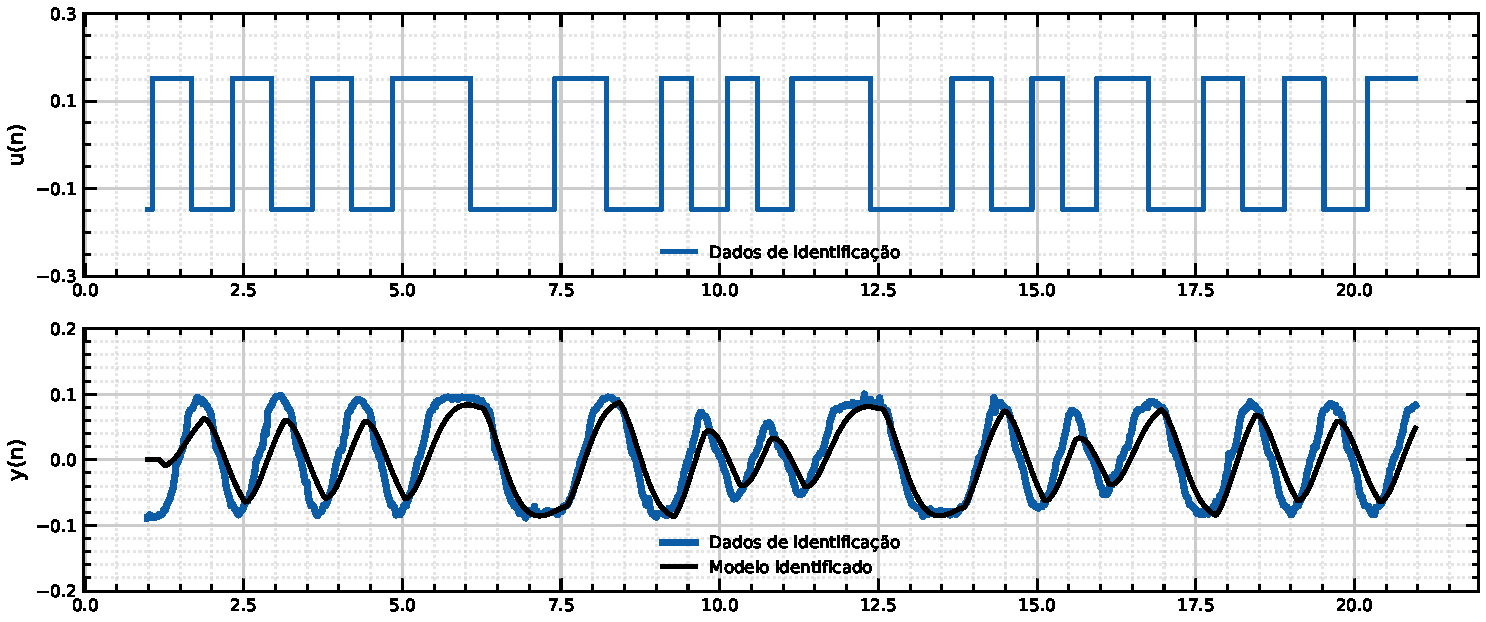
\includegraphics[width=1\textwidth]{Capitulos/3_1_resultados_discurcao/3_figuras/validacao_model_10grau.pdf}}
	\caption*{Fonte: elaborado pelo autor (2023).}
	\label{fig3:image_22}
\end{figure}


A partir de uma análise qualitativa entre o sinal de saída real e o simulado, figura \ref{fig3:image_22}, pode-se concluir que o modelo proposto a partir do método de mínimos quadrados teve exito, no entanto, ao modelar sistemas reais sempre haverá erro, isso por conta da não linearidade dos componentes físicos: sensores, atuadores e do próprio sistema, sedo assim, o modelo obtido é apenas uma aproximação do sistema real. %, para aplicar uma análise quantitativa, pode-se recorrer a alguns métodos de avaliação do modelo, para este exemplo, foi usado o Erro Quadrático Médio (EQM), equação \ref{eq3:eq4}.


\section{Ensaio em Malha Fechada com Controlador PID}
\label{malha_fechada}

O ecossistema desenvolvido possibilita aplicar diferentes controladores, bastando implementá-lo no formato de uma biblioteca e chamá-la no código principal do firmware, passando como parâmetro o erro que é calculado subtraindo da referência o valor lido na saída do sistema, isso permite maior flexibilidade ao pesquisador, que pode projetar diferentes controladores e realizar seus testes sem que seja necessário sobrescrever o código de implementação do sistema de controle, ou seja, a equação do controlador.

Com  proposito de testar o sistema em malha fechada, foi desenvolvido um controlador PID simples, tendo apenas um requisito, erro nulo para o sinal degrau. A figura \ref{fig3:image_23} exibe o diagrama do controlador proposto.% A equação \ref{eq3:eq5} exibe a estrutura do controlado já com os ganhos.


\begin{figure}[!h]
	\centering
	\caption{Sistema em Malha Fechada com Controlador PID.}
	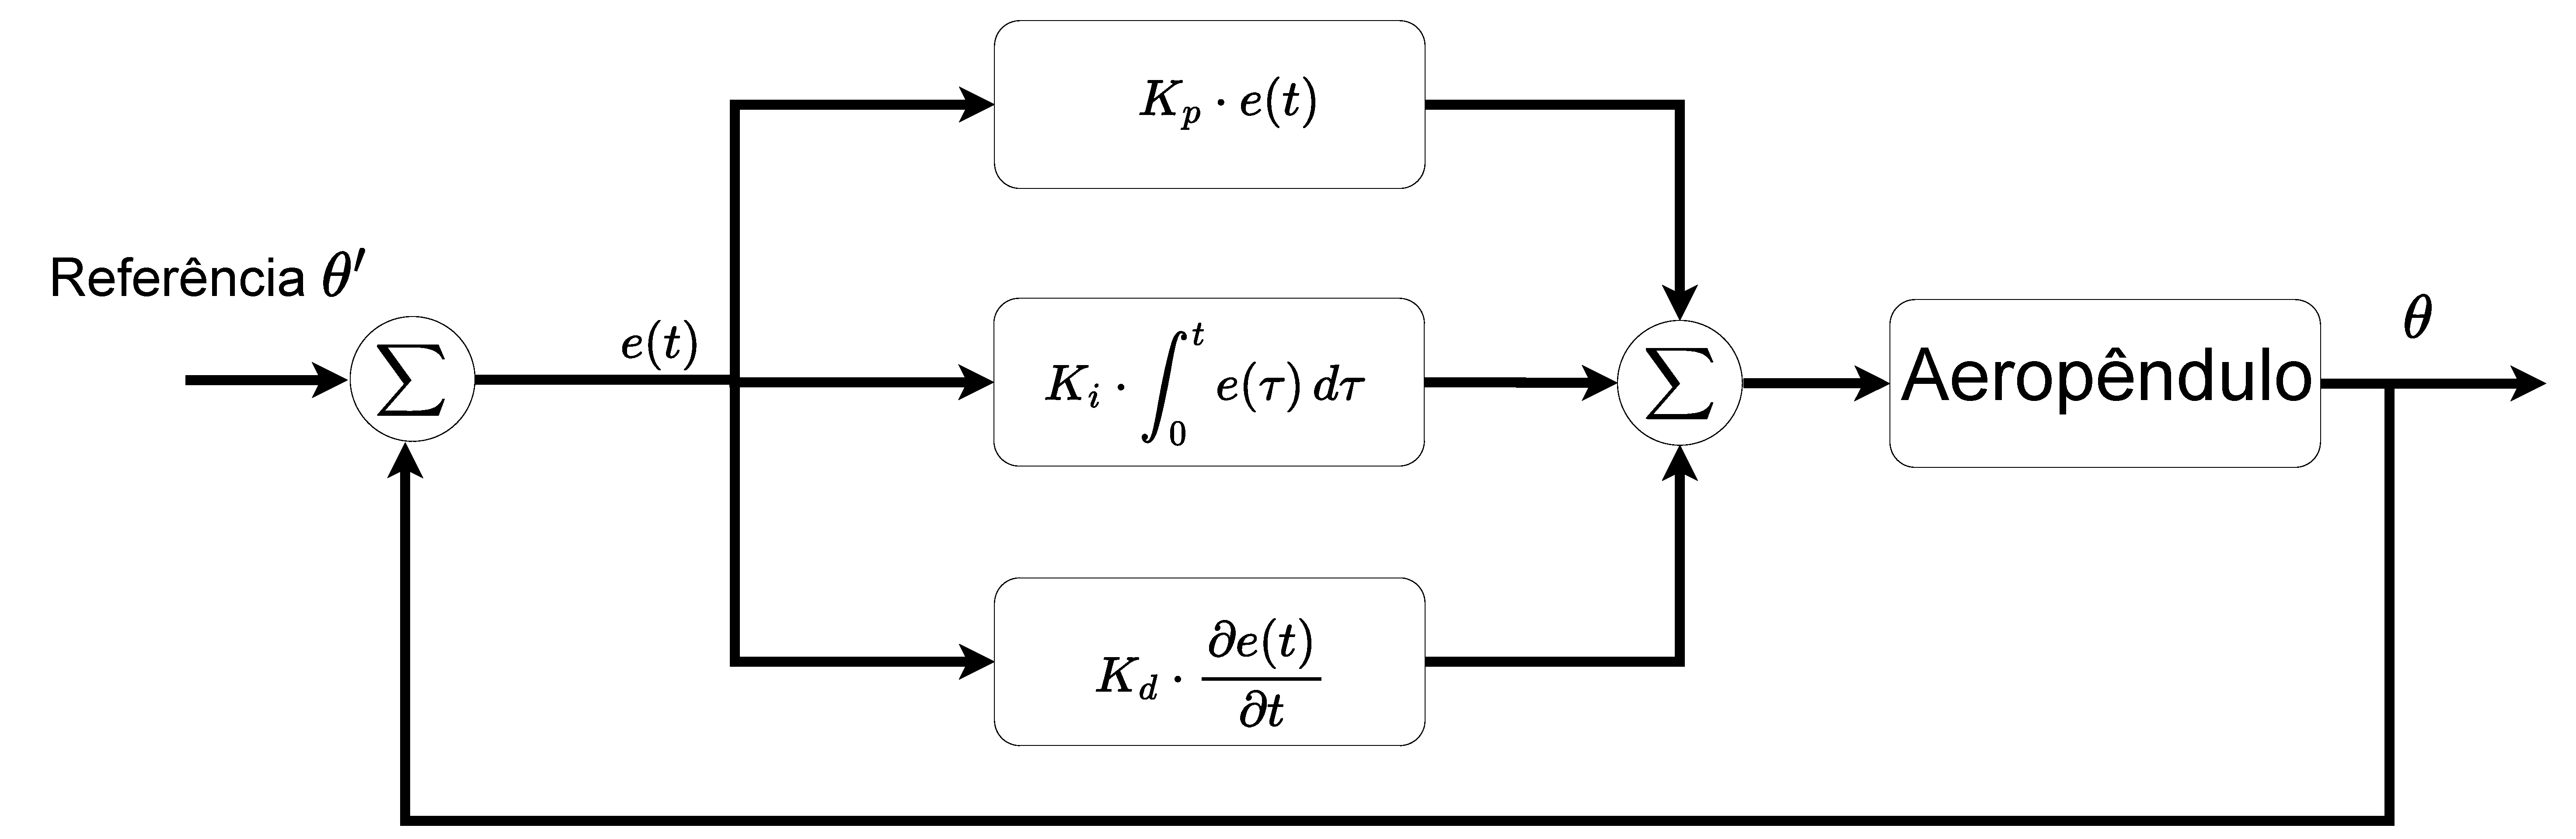
\includegraphics[width=1\textwidth]{Capitulos/3_1_resultados_discurcao/3_figuras/estrutura_pid.pdf}
	\caption*{Fonte: elaborado pelo autor (2023).}
	\label{fig3:image_23}
\end{figure}


No contexto da validação do sistema em malha fechada, optou-se por uma abordagem simplificada para a sintonia do controlador PID. Este método baseou-se na técnica de tentativa e erro. Após uma série de experimentos, determinaram-se os valores ótimos para os coeficientes do controlador, que foram os seguintes: $K_p=0,02$, $K_i=0,055$ e $K_d=0,35$.

% \begin{align}
% \frac{-0.0029 z^3 + 0.0023z^2 + 0.0016 z + 0.0097}{z^{10} - 0.9 z^9 - 0.3 z^8 - 0.014 z^7 + 0.13 z^6 + 0.15 z^5 + 0.012 z^4 - 0.05 z^3 - 0.12 z^2 - 0.02 z + 0.15}\quad dt = 0.02\label{eq3:eq5}
% \end{align}


\subsection{Onda Quadrada}

Ao inicializar a interface é possível escolher a opção de malha fechada, com isso a interface envia um comando para o microcontrolador que fecha a malha e aplica o sinal de controle na entrada do sistema, dessa forma, o aeropêndulo rasteia o sinal de referência escolhido, para o primeiro teste foi escolhido como sinal de referência uma onda quadrada com os seguintes parâmetros, frequência de 0,5 Hz, Amplitude 15° e offset de 1V. A figura \ref{fig3:image_24}, permite visualizar os sinais de referência e saída, ao analisá-los pode-se observar que o sinal de saída rasteia o sinal de referência. Além disso, observa-se que o sistema possui um transitório nas extremidades do sinal de onda quadrada, isso pode ser analisado a partir do sinal de erro que aumenta as extremidades do sinal de referência.

O gêmeo digital consome em tempo real o sinal angular do sistema real capturado através do potenciômetro, com isso é possível visualizar de uma forma gráfica a dinâmica do sistema real.

\begin{figure}[!h]
	\centering
	\caption{Gráficos dos Estados do Aeropêndulo com Controlador PID.}
	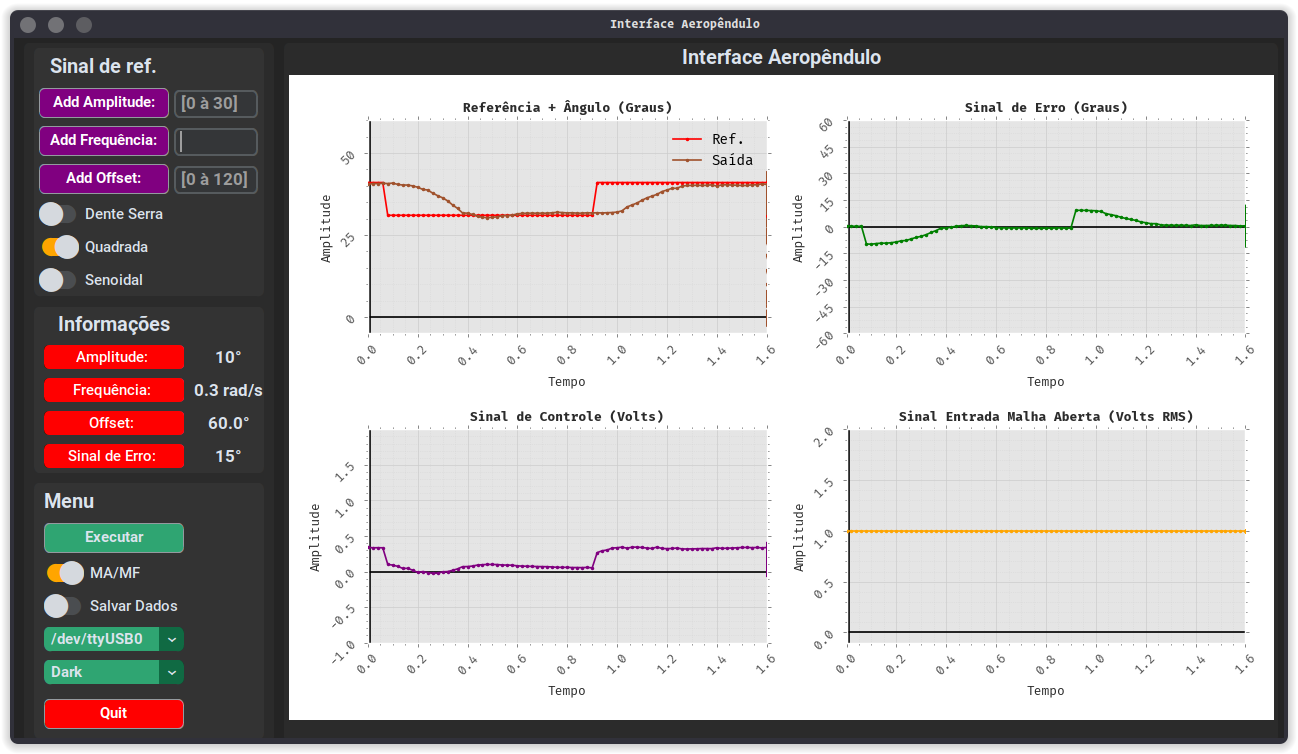
\includegraphics[width=0.9\textwidth]{Capitulos/3_1_resultados_discurcao/3_figuras/mf_gui_d1.png}
	\caption*{Fonte: elaborado pelo autor (2023).}
	\label{fig3:image_24}
\end{figure}


\begin{figure}[!h]
	\centering
	\caption{Gêmeo Digital com Controlador PID.}
	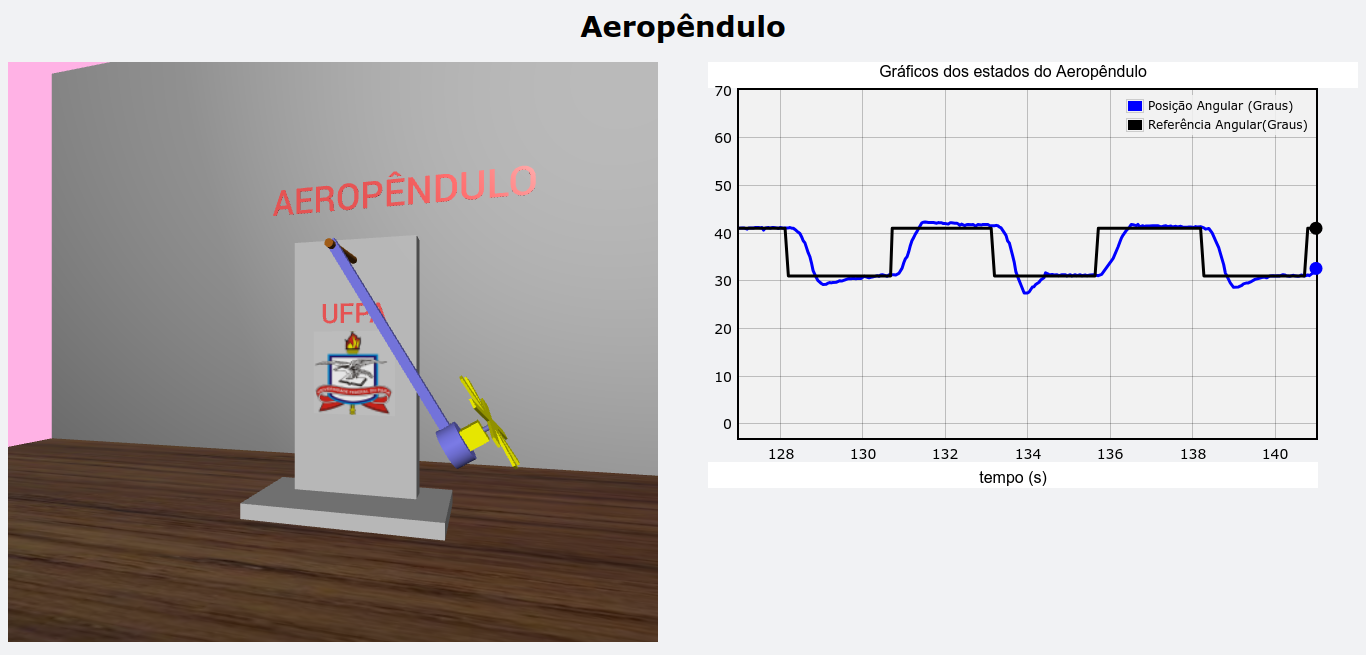
\includegraphics[width=0.9\textwidth]{Capitulos/3_1_resultados_discurcao/3_figuras/mf_gemeo_d1.png}
	\caption*{Fonte: elaborado pelo autor (2023).}
	\label{fig3:image_25}
\end{figure}


\subsection{Onda Dente de Serra}

Com o sinal de referência sendo uma onda dente de serra, pode-se observar que o controlador consegue rastreá-lo, tendo assim como no sinal degrau, um transitório nas extremidades.

\begin{figure}[!h]
	\centering
	\caption{Sistema em Malha Fechada com Controlador PID.}
	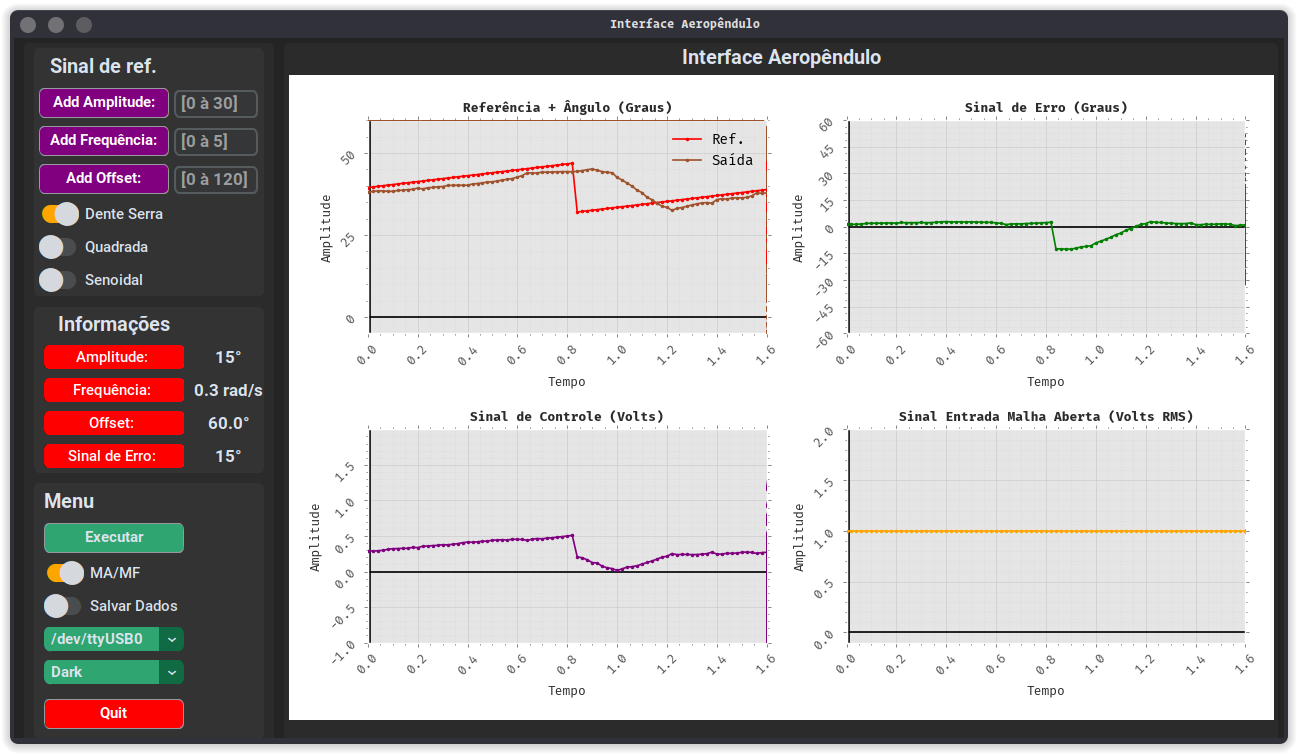
\includegraphics[width=0.9\textwidth]{Capitulos/3_1_resultados_discurcao/3_figuras/mf_gui_den1.png}
	\caption*{Fonte: elaborado pelo autor (2023).}
	\label{fig3:image_26}
\end{figure}


\begin{figure}[!h]
	\centering
	\caption{Gêmeo Digital consumindo os dados em tempo real do protótipo em Malha Fechada com Controlador PID.}
	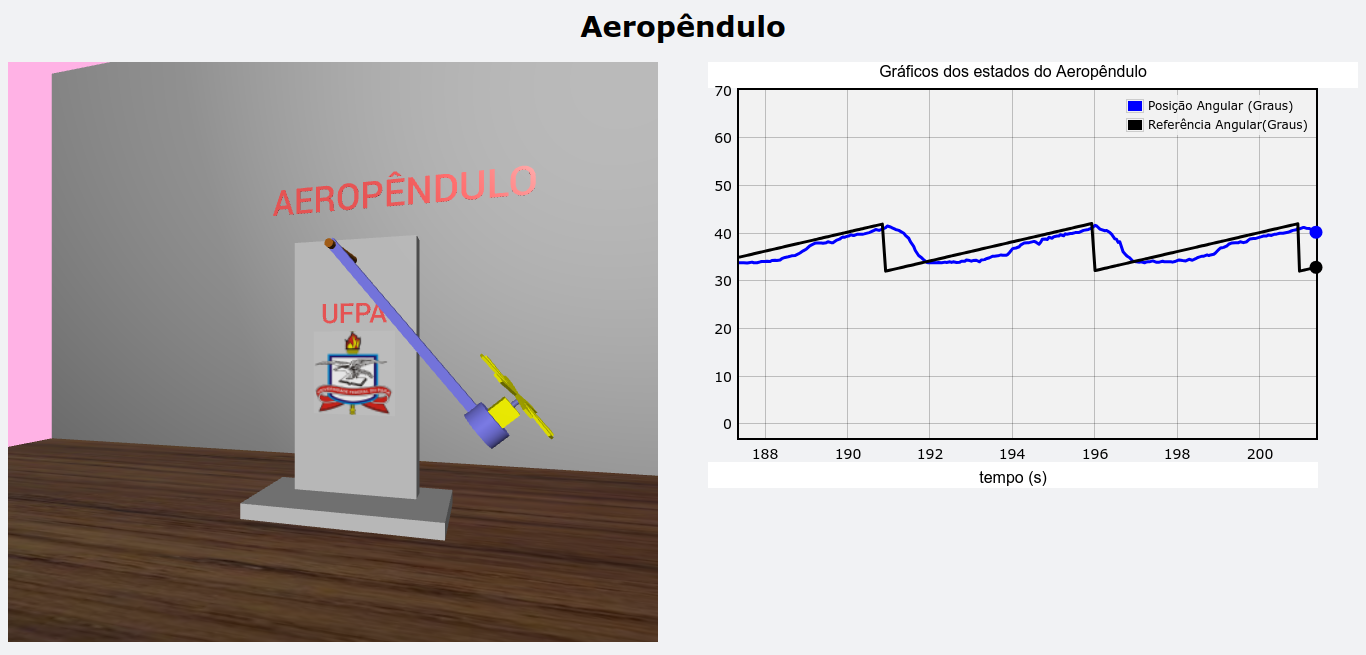
\includegraphics[width=0.9\textwidth]{Capitulos/3_1_resultados_discurcao/3_figuras/mf_gem_den1.png}
	\caption*{Fonte: elaborado pelo autor (2023).}
	\label{fig3:image_27}
\end{figure}




\chapter{Conclusão}
\label{cap_conclusao}

\section{Considerações Finais}
\label{concideracoes_finais}

Os subsistemas concebido para este projeto foi meticulosamente desenvolvido e testado, com resultados positivos abrangendo a modelagem matemática do sistema, a concepção e construção do protótipo, a elaboração do firmware, bem como o desenvolvimento dos softwares para a interface com o Aeropêndulo e a criação do gêmeo digital.

A modelagem matemática do sistema foi fundamentada nos princípios de Newton, no entanto, este processo demonstrou que a modelagem de sistemas pode rapidamente se tornar complexa e impraticável. Mesmo após a obtenção de um modelo que descreva a dinâmica do sistema, a determinação dos coeficientes finais pode ser uma tarefa árdua, uma vez que requer a utilização de sensores para obter tais grandezas, acrescentando uma camada de complexidade e desafios ao processo de modelagem. Dessa forma, o método de identificação de sistemas pode ser aplicado para encontrar um modelo matemático que aproxime a dinâmica do sistema real.


A concepção do protótipo foi meticulosamente planejada visando a simplificação do processo de construção. Com esse propósito em mente, a escolha recaiu sobre a utilização de materiais de custo reduzido para a estrutura e componentes eletrônicos amplamente disponíveis. Tal abordagem resultou na capacidade de replicar o sistema de forma eficaz e acessível, ampliando seu alcance não apenas para o público acadêmico, mas também para entusiastas interessados em sua implementação.


Após a implementação do laboratório virtual, foram conduzidos testes essenciais para validar o projeto. Inicialmente, adotou-se a técnica de identificação de sistema, que se mostrou eficaz na criação de um modelo com base nos dados de entrada e saída do sistema. Em uma etapa subsequente, aplicou-se um controlador PID em malha fechada para avaliar o corretor funcionamento do sistema em malha fechada. Ambos os testes foram bem-sucedidos, fornecendo evidências robustas de que os objetivos do projeto foram completamente alcançados. Com base nessas realizações, o projeto foi validado, estando pronto para ser implementado em disciplinas associadas a sistemas de controle. Além disso, sua aplicabilidade estende-se à condução de pesquisas acadêmicas, contribuindo significativamente para o avanço do processo de ensino e aprendizado na área de sistemas de controle.

Cabe destacar que os testes mencionados anteriormente não foram conduzidos com o intuito primário de obter resultados qualitativos ou quantitativos. Eles foram realizados exclusivamente como uma etapa de validação das funcionalidades desenvolvidas ao longo do projeto. Portanto, abre-se espaço para futuras pesquisas direcionadas à elaboração de modelos mais precisos e controladores mais robustos para o sistema, visando aprimorar ainda mais seu desempenho e eficácia.

\section{Trabalhos Futuros}
\label{trabalhos_futuros}

O projeto está agora concluído e totalmente preparado para ser aplicado em diversas áreas de pesquisa. Essa versatilidade permite a realização de estudos em identificação de sistemas, explorando diferentes métodos. Além disso, é viável o desenvolvimento de controladores por meio de abordagens clássicas ou com o uso de inteligência artificial, incluindo técnicas de aprendizagem por reforço, deep Q-learning e outros algoritmos relevantes. Além disso, a expansão do laboratório virtual é factível, permitindo a incorporação de novas funcionalidades tanto na interface gráfica quanto no próprio protótipo.

O projeto avançará com a elaboração de uma documentação abrangente, a qual será disponibilizada online através do GitHub, apêndice \ref{apendice_1}. Além disso, o recurso será completado com a criação de vídeos explicativos que detalharão cada aspecto do projeto. É importante destacar que o projeto será de código aberto, aberto a contribuições de pesquisadores, estudantes e entusiastas. Essa abertura colaborativa permitirá um contínuo aprimoramento ao longo do tempo. Dessa forma, nosso objetivo é estabelecer um ambiente de pesquisa abrangente e acessível, promovendo a ampla disseminação do conhecimento na comunidade acadêmica e além dela.

% ---
% Capítulo 03 - Desenvolvimento
%% REVISÃO DE LITERATURA-------------------------------------------
\chapter{DISPOSITIVOS LÓGICOS E LÓGICA PROGRAMÁVEL}
\label{cap2}


\begin{figure}[!htb]
    \centering
    \caption{A estrutura de uma descrição VHDL com os seus blocos}
    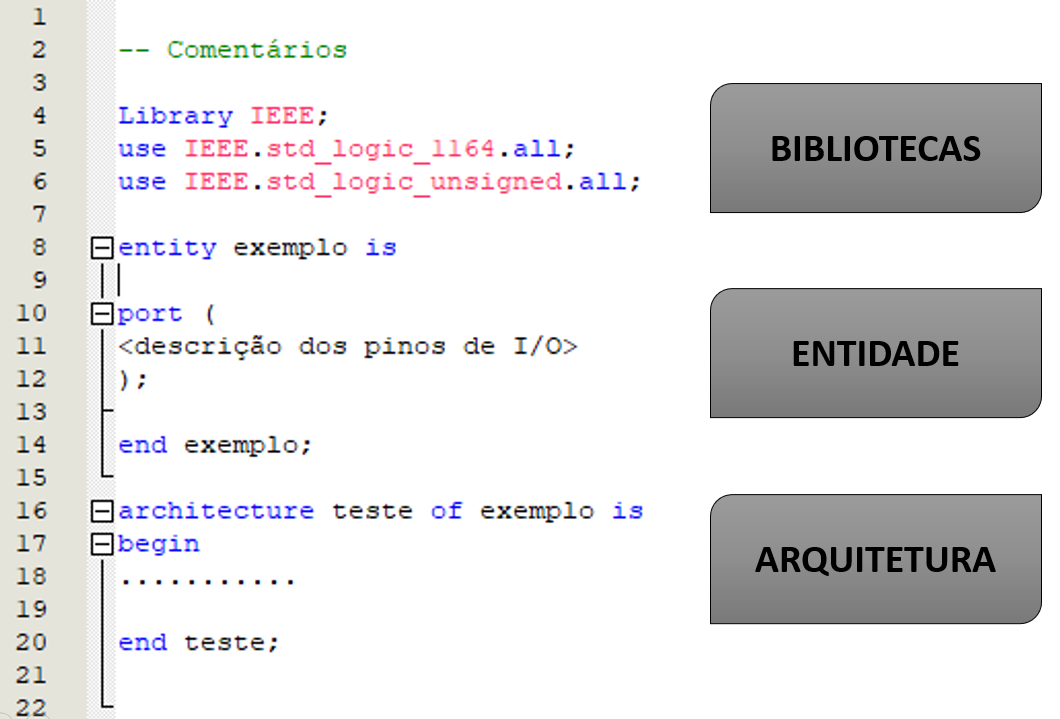
\includegraphics[height = 9cm]{figuras/estrut_blocVHDL.png}\\
    {\footnotesize Fonte: Autoria própria.}
    \label{fig:vhdl_blocos_estrut}
\end{figure}
 
\subsubsection{Declaração de biblioteca e Pacotes}

As bibliotecas e os pacotes são conjuntos de declarações usadas para um determinado fim. Pode ser um conjunto de subprogramas, ou funções que operem com um tipo de dado, assim como pode ser um conjunto de declarações necessárias para modelar um determinado projeto. Uma biblioteca é usada para organizar e gerenciar diferentes unidades de design em um projeto VHDL. É comum criar diferentes bibliotecas para organizar e armazenar unidades de design relacionadas. Por exemplo, uma biblioteca pode ser criada para armazenar unidades de design relacionadas a interface serial, enquanto outra biblioteca pode ser criada para armazenar unidades de design relacionadas a processamento de sinais \cite{roth2004circuit}.

Os pacotes são usados para definir e compartilhar constantes, tipos de dados, funções, procedimentos e outras construções que podem ser usadas em várias unidades de design. Os pacotes podem ser usados para evitar a repetição de código e facilitar a reutilização de código em diferentes unidades de design \cite{ordonez2003projeto}. Por exemplo, um pacote pode ser criado para definir um tipo de dado personalizado que é usado em várias unidades de design. 
Bibliotecas e Pacotes mais utilizados estão citados no quadro \ref{quadro_1}.
%+++++++++++++++++++++++++++++++++++++++++++++++

\begin{quadro}[h]
    \caption{Pacotes mais utilizados (Biblioteca IEEE)}
    \label{quadro_1}
    \centering
     \begin{tabular}{|c|p{3cm}|p{8cm}|}
      \hline
      \textbf{Pacote} & \textbf{Tipos de dados} & \textbf{Descrição} \\
      \hline
      std\_logic & std\_logic e std\_logic\_vector & Define o padrão para descrever a interconexão entre tipos de dados usados na linguagem VHDL \\
      \hline
       std\_logic\_arith & Especifica tipos de dados sinalizados e não sinalizados & Funções de conversão, operações aritméticas e comparações para uso de dados sinalizados e não sinalizados \\
      \hline
       std\_logic\_unsigned & std\_logic\_vector & Define funções que permitem usar tipos de dados std\_logic\_vector, como se fossem tipo de dado não sinalizado \\
      \hline
       std\_logic\_signed & std\_logic\_vector & Define funções que permitem usar tipos de dados std\_logic\_vector, como se fossem tipo de dado sinalizado \\
      \hline
       numeric\_std & & Substitui os pacotes usados juntos std\_logic\_atith, std\_logic\_unsigned e std\_logic\_signed \\
      \hline                 
    \end{tabular}
  \vspace{1.5pt}
  \caption*{\footnotesize Fonte: \cite{ordonez2003projeto}}
\end{quadro}

A declaração do uso de pacotes e bibliotecas é mostrada no quadro \ref{quadro_2}. O uso de .all implica que todos os elementos da biblioteca podem ser usados.


\subsubsection{Declaração de Entidade}

\begin{table}[htb]
\ABNTEXfontereduzida
\center \caption{Parâmetros da Condutividade Intrabanda do Grafeno \cite{b5}\cite{b13}}
\label{Tab1}
\vline  \begin{tabular}{p{0.6cm}|p{2cm}|p{2cm}|p{6cm}}
  \hline
   \textbf{ } & \textbf{Valor}  & \textbf{Unidade}  & \textbf{Descrição}  \\
   \hline
	\hline
$e$  &  $1,60\times10^{-19}$  &   $C$  &    Carga do Elétron\\
$\hbar$   &   $1,05\times10^{-34}$ & $J\!\cdot\!s/rad $ & Constante de Plank Reduzida\\
$k_B$   &   $1,38\times10^{-23}$ & $J/K $ & Constante de Boltzmanm\\
$T$   &   $300$ & $K$ &  Temperatura\\
$\sigma_0$   &   $e^2/4\hbar$ & $S\!\cdot\!rad$ & Condutividade HF\\
$\mu_c$   &   $0; 0,25; 0,5$ & $eV$ & Potencial Químico\\
$\tau$   &   $0,5$ & $ps$ & Tempo de Amortecimento\\
\hline

\end{tabular}\vline  
\end{table}

\begin{equation}\label{eq3.2}
\textbf{E}_1(x,z) = -\hat{a}_y\left[E_{iy}e^{-jk_{z1}(z+d_1)} + E_{ry}e^{+jk_{z1}(z+d_1)}\right]e^{-jk_x x}  
\end{equation}
% ---


%-------------------------------------Elementos pós-textuais:-------------------------------------
\postextual
%Referências Bibliográficas:
%Opção 1 - Preenchendo manualmente as referências:
%% REFERÊNCIAS------------------------------------------------------------------

\begin{thebibliography}{00}
\bibitem{b1} M. A. Cooper, Optical biosensors in drug discovery. Nature Reviews Drug Discovery. 1:515-528, 2002.

\bibitem{b2} D. W. Pohl, A. Alu, N. Engheta $\&$ F. Marquier, Optical Antennas. Forthcoming Publications: Science, PRL, 2013.

\bibitem{b3} R. Marani, M. Grande, V. Petruzelli $\&$ A. DOrazio, Plasmonic bandgaps in 1D arrays of slits on metal layers excited by out-of-plane sources, International Journal of Optics, Hindawi, 2012.

\bibitem{b4} H. S. P. Wong $\&$ D. Akinwande. Carbon nanotube and graphene device physics. Cambridge University Press, 2011.

\bibitem{b5} P. A. D. Gonalves, $\&$ N. M. Peres. An introduction to Graphene plasmonics. 2016.

\end{thebibliography} 
%.................................................................................................
%Opção 2 - Utilizando Bibtex (Melhor opção):
\bibliographystyle{abntex2-alf} % Define o estilo ABNT para formatar a lista de referências 
\bibliography{bibtex-referencias}
%Passos: Abrir o arquivo bib_tex-referencias, adcionar as referências a partir do Google Acadêmico, pressionar F11 duas vezes.  Antes de compilar o arquivo tex. pressionar F11 duas vezes para rodar o arquivo bib, e então compilar, de preferências duas vezes.

%.................................................................................................
% ---
%Insere os apêndices:
% APÊNDICES--------------------------------------------------------------------

\begin{apendicesenv}
\partapendices

% Primeiro apêndice------------------------------------------------------------
\chapter{Nome do apêndice} % Edite para alterar o título deste apêndice
\label{chap:apendiceA}

Lembre-se que a diferença entre apêndice e anexo diz respeito à autoria do texto e/ou material ali colocado.

Caso o material ou texto suplementar ou complementar seja de sua autoria, então ele deverá ser colocado como um apêndice. Porém, caso a autoria seja de terceiros, então o material ou texto deverá ser colocado como anexo.

Caso seja conveniente, podem ser criados outros apêndices para o seu trabalho acadêmico. Basta recortar e colar este trecho neste mesmo documento. Lembre-se de alterar o "label"{} do apêndice.

Não é aconselhável colocar tudo que é complementar em um único apêndice. Organize os apêndices de modo que, em cada um deles, haja um único tipo de conteúdo. Isso facilita a leitura e compreensão para o leitor do trabalho.

% Novo apêndice----------------------------------------------------------------
\chapter{Nome do outro apêndice}
\label{chap:apendiceB}

conteúdo do novo apêndice

\end{apendicesenv}
             		   
% ---
% Insere os anexos:
%% ANEXO------------------------------------------------------------------------

\begin{anexosenv}
\partanexos

% Primeiro anexo---------------------------------------------------------------
\chapter{Nome do anexo}     % edite para alterar o título deste anexo
\label{chap:anexoA}

Lembre-se que a diferença entre apêndice e anexo diz respeito à autoria do texto e/ou material ali colocado.

Caso o material ou texto suplementar ou complementar seja de sua autoria, então ele deverá ser colocado como um apêndice. Porém, caso a autoria seja de terceiros, então o material ou texto deverá ser colocado como anexo.

Caso seja conveniente, podem ser criados outros anexos para o seu trabalho acadêmico. Basta recortar e colar este trecho neste mesmo documento. Lembre-se de alterar o "label"{} do anexo.

Organize seus anexos de modo a que, em cada um deles, haja um único tipo de conteúdo. Isso facilita a leitura e compreensão para o leitor do trabalho. É para ele que você escreve.

% Novo anexo-------------------------------------------------------------------
\chapter{Nome do outro anexo}
\label{chap:anexoB}

conteúdo do outro anexo

\end{anexosenv}
               		  
% ---
%Para conhecimento: Apêndices são textos elaborados pelo autor a fim de complementar sua argumentação. Anexos são os documentos não elaborados pelo autor, que servem de fundamentação, comprovação ou ilustração, como mapas, leis, estatutos etc.
% -------------------------------------------------------------------------------------------------
\end{document}
